% se puede agregar la opción [english] para 
% memorias o tesis en inglés (borrando el archivo .aux)
\documentclass[english]{umemoria}
%\documentclass{umemoria}
\pdfminorversion=7 % permite incluir PDFs versión 1.7 (evita el warning de PDF inclusion)

\depto{Departamento de Ingeniería Eléctrica}
\author{Ignacio Romero Aravena}
\title{Mitigating Catastrophic Forgetting in Object Classification Via Gaussian Class Representations}

% incluir ambos comandos para una doble titulación
%  o quitar el comando que no aplica
\memoria{Ingeniero Civil Eléctrico} % en caso de doble grado
\tesis{Magíster en CIENCIAS DE LA INGENIERÍA, MENCIÓN ELÉCTRICA} % en caso de magíster
%\tesis{DOCTOR[A] EN INGENIERÍA ELÉCTRICA} % incluir solo este comando para doctorados

% puede haber varios profesores guía seperados por coma;
% pero si es una memoria, solo puede haber un profesor guía
\guia{Javier Ruiz Del Solar} 

% puede haber varios profesores co-guía seperados por coma;
% pero si es una memoria, el profesor co-guía será el primer
% integrante de la comisión
\coguia{Patricio Loncomilla} % incluir en caso de co-guía de *tesis*

%\cotutela{Nombre Institución} % incluir en caso de cotutela

\comision{Jorge Silva, Rodrigo Verschae}

\auspicio{FONDECYT 1251823} % incluir en caso de recibir financiamiento

% tiene que ser el año en que se da el examen de título/grado (defensa)
\anho{2026} % incluir solo para reemplazar el año actual

%%%%%%%%%%%%%%%%%%%%%%%%%%%%%%%%%%%%%%%
% Paquetes extra:

% Glosario 
\usepackage[acronym,nomain,nonumberlist]{glossaries}
\makeglossaries
\renewcommand*{\glsgroupskip}{}

% Para las captions con diferente título en texto y en índice
\newcommand{\mycaption}[2]{\caption[{#1}]{#2}}

% Figuras TikZ
\usepackage{tikz}
\usetikzlibrary{arrows.meta, positioning, shapes.geometric}
\usepackage{tikz}

% Algoritmos
\usepackage{algorithm2e}
\iflanguage{spanish}{
    \renewcommand{\algorithmcfname}{Algoritmo}
}{
    \renewcommand{\algorithmcfname}{Algorithm}
}

% Subfiguras
\usepackage{subcaption}

% Logo de Github
\usepackage{fontawesome5}

% Tablas: \toprule/\midrule/\bottomrule, tabularx, multirow,
% \rowcolor y \begin{adjustbox} usados en los capítulos de resultados
\usepackage{booktabs}
\usepackage{array}
\usepackage{tabularx}
\usepackage{multirow}
\usepackage[table]{xcolor}
\usepackage[export]{adjustbox}

%%%%%%%%%%%%%%%%%%%%%%%%%%%%%%%%%%%%%%%

\begin{document}

\frontmatter
\maketitle

  \noindent\hfill
 \begin{minipage}[t]{0.6\textwidth}
 	%RESUMEN DE LA TESIS PARA OPTAR AL \\
 	%GRADO DE DOCTOR[A] EN INGENIERÍA \\
 	%ELÉCTRICA, \\
 	RESUMEN DE LA TESIS PARA OPTAR AL \\
 	GRADO DE MAGÍSTER EN CIENCIAS DE LA \\ INGENIERÍA, MENCIÓN ELÉCTRICA, \\
 	MEMORIA PARA OPTAR AL TÍTULO DE \\ INGENIERO CIVIL ELÉCTRICO \\
 	{POR: IGNACIO ROMERO ARAVENA} \\
 	{FECHA: \the\year} \\
 	{PROF. GUÍA: JAVIER RUIZ DEL SOLAR} \\
 	{PROF. CO-GUÍA: PATRICIO LONCOMILLA}
 \end{minipage}
 
 \begin{center}
 	MITIGACIÓN DEL OLVIDO CATASTRÓFICO EN LA CLASIFICACIÓN DE OBJETOS MEDIANTE REPRESENTACIONES GAUSSIANAS DE CLASES
 \end{center}
 
 \noindent Los modelos tradicionales de aprendizaje profundo suelen fallar al trabajar con datos no estacionarios: incorporar clases nuevas exige un reentrenamiento costoso o se olvida lo ya aprendido. Para resolverlo, se presenta un método de aprendizaje incremental por clases libre de gradientes, que aborda el reconocimiento visual continuo mediante la estimación de densidades en forma cerrada, en lugar de la optimización de parámetros. A partir de las representaciones de un extractor de características DINOv2 congelado, cada clase se modela mediante una distribución gaussiana multivariada. Las clases nuevas se integran al instante, sin necesidad de retropropagación, almacenamiento de muestras ni ajuste de parámetros. Como la información de las clases anteriores nunca se altera, el sistema previene el olvido por diseño. Evaluado en Split CIFAR-100, Split ImageNet-R, Split Caltech-256 y en un benchmark conjunto de 30 tareas, este enfoque determinista iguala o supera a los métodos basados en prompts que requieren optimización. La variante MOG4-Shared —que combina una mezcla de gaussianas por clase con una covarianza compartida— ofreció el mejor desempeño. Finalmente, un análisis estadístico del espacio de características de valida el supuesto gaussiano y demuestra que la covarianza ideal depende de la cantidad de datos disponibles por clase.
 %%%%%%%%%%%%%%%%%%%%%%%%%%%%%%%%%%%%%%%
 % SÓLO PARA TESIS EN INGLÉS 
 % BORRAR EN CASO DE ESCRITURA EN ESPAÑOL
 \newpage
 
 \noindent\hfill
 \begin{minipage}[t]{0.6\textwidth}
 	%RESUMEN DE LA TESIS PARA OPTAR AL \\
 	%GRADO DE DOCTOR[A] EN INGENIERÍA \\
 	%ELÉCTRICA, \\
 	RESUMEN DE LA TESIS PARA OPTAR AL \\
 	GRADO DE MAGÍSTER EN CIENCIAS DE LA \\ INGENIERÍA, MENCIÓN ELÉCTRICA, \\
 	MEMORIA PARA OPTAR AL TÍTULO DE \\ INGENIERO CIVIL ELÉCTRICO \\
 	{POR: IGNACIO ROMERO ARAVENA} \\
 	{FECHA: \the\year} \\
 	{PROF. GUÍA: JAVIER RUIZ DEL SOLAR} \\
 	{PROF. CO-GUÍA: PATRICIO LONCOMILLA}
 \end{minipage}
 
 \begin{center}
 	MITIGATING CATASTROPHIC FORGETTING IN  OBJECT CLASSIFICATION VIA GAUSSIAN CLASS REPRESENTATIONS
 \end{center}
 
 \noindent Traditional deep learning models struggle with non-stationary data: adding new categories usually means costly retraining or forgetting what came before. This thesis presents a gradient-free class-incremental learning framework that treats lifelong visual recognition as closed-form density estimation instead of parameter optimization. A frozen DINOv2 encoder is paired with per-class multivariate Gaussian models. New classes are added instantly without backpropagation, sample storage, or tuning. Because past class statistics are never touched, the framework avoids representation drift and forgets nothing by construction. Tested on Split CIFAR-100, Split ImageNet-R, Split Caltech-256, and a 30-task Joint benchmark mixing all three, this deterministic approach matches or beats optimization-heavy, prompt-based methods. MOG4-Shared, combining a small per-class mixture with one shared covariance, is the strongest configuration once cost and consistency are weighed together. A statistical study of the DINOv2 embedding space, using normality tests, spectral analysis, and Bhattacharyya distances, supports the Gaussian assumption behind the method and shows that the best covariance choice depends on how much data each class has.
 

 %En el caso de redactar la tesis en inglés, se debe incluir un resumen adicional en dicho idioma con su título en inglés, ya que el resumen en español (con título en español) es obligatorio independientemente del idioma de la tesis. Ambos resúmenes deben reflejar el mismo contenido. Sin embargo, dado que cada uno debe cumplir independientemente con el límite de doscientas (200) palabras, no es necesario que sean una traducción textual el uno del otro. Las mismas recomendaciones estructurales indicadas en el resumen anterior aplican para ambos.


\begin{dedicatoria}
A los completos con Coca Zero
\end{dedicatoria}

\begin{thanks}
A mi mamá y mi papá, por siempre confiar en mí y darme todas las herramientas para lograr lo que quiera en la vida. Son los mejores papás que he tenido, los amo un huevo.

A mi hermana, la persona que más amo en el mundo. Todo lo que soy, voy a ser, he logrado y voy a lograr, es para ti.

A Lili, Miguelín, Máximo y la guagüita que viene en camino. A la Loreto. A mi tata, Yaqui, mi mami y la tía Ketita. La familia no se escoge, pero yo los voy a escoger siempre.
 
Al Charly, el Tony, Conbotas, y la Princesa. Por dejarme amarlos y por acompañarme.

A la Isi y a la Amandita: el mejor regalo que me entregó la universidad, mis mejores amigas. Por ser luz y alegrar mis días.

A mis amigos de la vida: Mariancita, Máximo, Meza, Sophia, Andrés, Cristóbal, Benja, Germán, Lucase, Kavi, Sofía Amapola, Vale, Luna, Jorge, Felipe, Vane, Renatito, Javi, Nachita. Sin ustedes la vida no sería la misma.

A los ETs: Caba, Day, Camilo, Cristian, JP, Enzo, Brunos, Danae, Anto, Titin, Rorro, Cami, Kakame, Andrew, los antiguos, los nuevos y los que vendrán. Gracias por jugársela.

A mis rompehogares: Gonz, Matti, Sebita, Lucho, Sahian, Fer, Rona, Bruno, Felipe, Pipe. Por los chistecitos a la hora de almuerzo, el apañe académico, Mario Kart, cartitas pokémon y tantas otras ñoñerías que hemos pasado juntos.

Al deporte: a la rama de natación, Pace One y Stravamigos. Pionxi, Oscar, Simón, Javis, Martín, Sofi, Edgar, Seba, Jo, Pía, Macami, Rick, Nico, profe Moni, coaches Salazar, Cami y tantos compañeros y compañeras de entrenamiento. Porque no existen los deportes individuales, son el mejor equipo que puedo pedir.

A mis profesores, por entregarme una formación que fue más allá de artes, ciencias o lenguas. Siempre estaré muy agradecido de haber pasado por sus salas de clase: Profesora Irma Meza, profesora Yarith Jorrat, profesor Harold Leiva, profesora Súa Vicencio, profesora María Isabel Caqueo, profesor Felipe Muñoz, profesor Joaquín Álvarez.

Al profesor Javier y a Pato Loncomilla: gracias por confiar en mí.


Y finalmente a mi amigo Jesús, por acompañarme en el camino y enseñarme que la medida del amor, es amar sin medidas.

\end{thanks}

\chapter*{Declaración y uso de IA}
\markboth{Declaración y uso de IA}{Declaración y uso de IA}

Para la redacción y estructuración de esta tesis se empleó Claude, herramienta de
inteligencia artificial generativa de Anthropic, a través de la plataforma Claude Code. Su uso
se enfocó en la redacción y refinamiento de contenidos para los capítulos de introducción,
estado del arte, marco teórico, metodología y resultados. Asimismo, la herramienta asistió en
la revisión gramatical, la reorganización y jerarquización de secciones, y la elaboración tanto
del resumen ejecutivo como de las descripciones para tablas e ilustraciones.
Las instrucciones proporcionadas fueron descriptivas y contextuales, tales como “reescriba
el texto para que sea más claro y conciso”, “resuma la sección en un párrafo de 5 líneas”,
“reorganice la sección para que tenga una estructura más lógica”, “escriba un resumen ejecutivo que capture problema, arquitectura, pruebas experimentales y contribuciones”.
El autor revisó y validó todo el contenido antes de su incorporación. Cada afirmación
técnica se contrastó con datos experimentales y arquitectura efectivamente implementada.
Se verificó coherencia entre secciones, consistencia de notación y línea argumental. Los fragmentos que no correspondían al estilo o nivel de detalle fueron reescritos, y el autor incorporó
datos cuantitativos, referencias bibliográficas y detalles de implementación. Cada capítulo fue
revisado completamente para confirmar que análisis y conclusiones corresponden al criterio
del autor.
El autor revisó y validó todo el contenido de esta memoria. La herramienta se utilizó como
apoyo al trabajo intelectual y no figura como coautora. La responsabilidad académica sobre
los resultados, análisis y conclusiones presentados corresponde íntegramente al autor.

\tableofcontents
\listoftables % opcional
\listoffigures % opcional

%\input{Capitulos/Glosario} % opcional

\mainmatter
\chapter{Introduction}
\label{ch:intro}

\section{Motivation}

State-of-the-art (SOTA) object classification methods rely on deep learning models that are either trained end-to-end on the target application or initially trained on one task and subsequently fine-tuned for a different one. In both cases the resulting models are \emph{monolithic}: a single network is trained on a large dataset and performs feature extraction and classification jointly. Such models are highly effective when the set of object classes is fixed and known at training or fine-tuning time. When new object classes must be incorporated, however, the entire model must be retrained or fine-tuned. This procedure requires significant computational resources, demands access to the original training dataset and, in many cases, leads to \emph{catastrophic forgetting} of previously learned classes \cite{catastrophic}.

A natural way to integrate new classes while avoiding catastrophic forgetting is to formulate the problem as continual or class-incremental classification, in which the algorithm must learn to distinguish an ever-growing number of categories \cite{vandeVen}. In this paradigm, a \emph{task} corresponds to a distinct portion of the training experience, presented sequentially to the model. Instead of having access to the entire dataset at once, as in conventional supervised learning, the model receives data in sequential chunks \cite{taskarithmeticloracontinual}. Each task typically corresponds to a set of new classes that must be recognised. The central challenge is that when the model is updated task by task, it tends to overwrite previously acquired knowledge: monolithic models are structurally ill-suited for this scenario, and an alternative paradigm is therefore required.

This limitation has motivated the SOTA in continual classification to focus on balancing \emph{stability} and \emph{plasticity}. Stability refers to a model's ability to preserve previously learned knowledge; plasticity describes its capacity to adapt and incorporate new tasks \cite{API}. Traditional approaches rarely optimise both properties simultaneously: when stability dominates, the model struggles to integrate new knowledge; when plasticity dominates, it loses access to past information. This trade-off is compounded by the limited capacity of neural networks to integrate new representations without interfering with old ones and by the need to continually adjust the network's structure to match the growing number of object classes. The dominant view in the literature therefore treats continual learning as a problem of \emph{parameter interference}: learning new classes requires updating network weights, which may overwrite previously acquired knowledge, and most existing methods attempt to control this process through regularization, rehearsal buffers, or architectural adaptations \cite{CL}. Although effective, these strategies share a common premise that this thesis sets out to challenge: that incremental learning must be achieved through continuous, careful optimization of the parameters of the network responsible for feature extraction.

This premise diverges significantly from the organisational principles of biological vision. The human visual system relies on early cortical regions responsible for feature extraction that mature and stabilize during the initial postnatal weeks or months~\cite{Sluyters90}, providing highly stable feature representations that remain stationary throughout adulthood. However, despite this invariant sensory foundation, human lifelong learning persists. Higher-order cognitive systems seamlessly map these fixed perceptual representations onto newly encountered semantic categories, even if acquiring knowledge of a new object class can occasionally result in a slight, localized reduction in the ability to distinguish highly similar classes over time.

 
A directly analogous structural separation has recently become achievable in computer vision through large-scale visual foundation models. By leveraging pre-trained foundation models such as DINOv2 \cite{oquab2024dinov}—which are trained on massive, diverse datasets—downstream systems obtain highly discriminative representations that remain completely stable once frozen. In this stationary feature space, \emph{representation drift}—the gradual shifting of a network's internal features during sequential task updates, which serves as the primary driver of catastrophic forgetting—is eliminated by construction: the coordinates describing each class no longer change when a new task arrives. Mirroring the biological paradigm, class-incremental learning can thus be conceptually reframed: rather than protecting network parameters from destructive interference, the challenge becomes one of accurately modeling the distribution of new classes within a robust, fixed embedding space. This perspective motivates the present work: once a sufficiently discriminative and stable feature space is secured, the core challenge of continual learning shifts from \emph{preventing forgetting} to \emph{estimating probability densities}.

Building on this observation, this thesis proposes a continual-learning object-recognition system organized into two complementary, decoupled components. As illustrated in Figure~\ref{fig:intro_overview}, the first component is a \emph{feature extractor} derived from a frozen, pre-trained foundation model. This encoder maps an input image to a static, highly discriminative feature vector $\vec{x}$ in a shared embedding space. Crucially, these representations must be sufficiently general to characterize arbitrary object classes, including those unseen during the foundation model's pre-training. The second component is a \emph{statistical classifier} composed of a collection of independent, class-conditional Gaussian models ($G_1, \dots, G_N$). When a new class arrives, a corresponding Gaussian model is estimated and integrated without altering or accessing previously learned class models. At inference time, classification is performed by computing the posterior probability $p(c_k \vert{} \vec{x})$ for each class and assigning the input to the class that yields the maximum value, in direct analogy to a generative Bayes classifier. This modular, two-stage framework is developed in full mathematical detail in Chapter~\ref{methodology}.

\begin{figure}[htb]
	\centering
	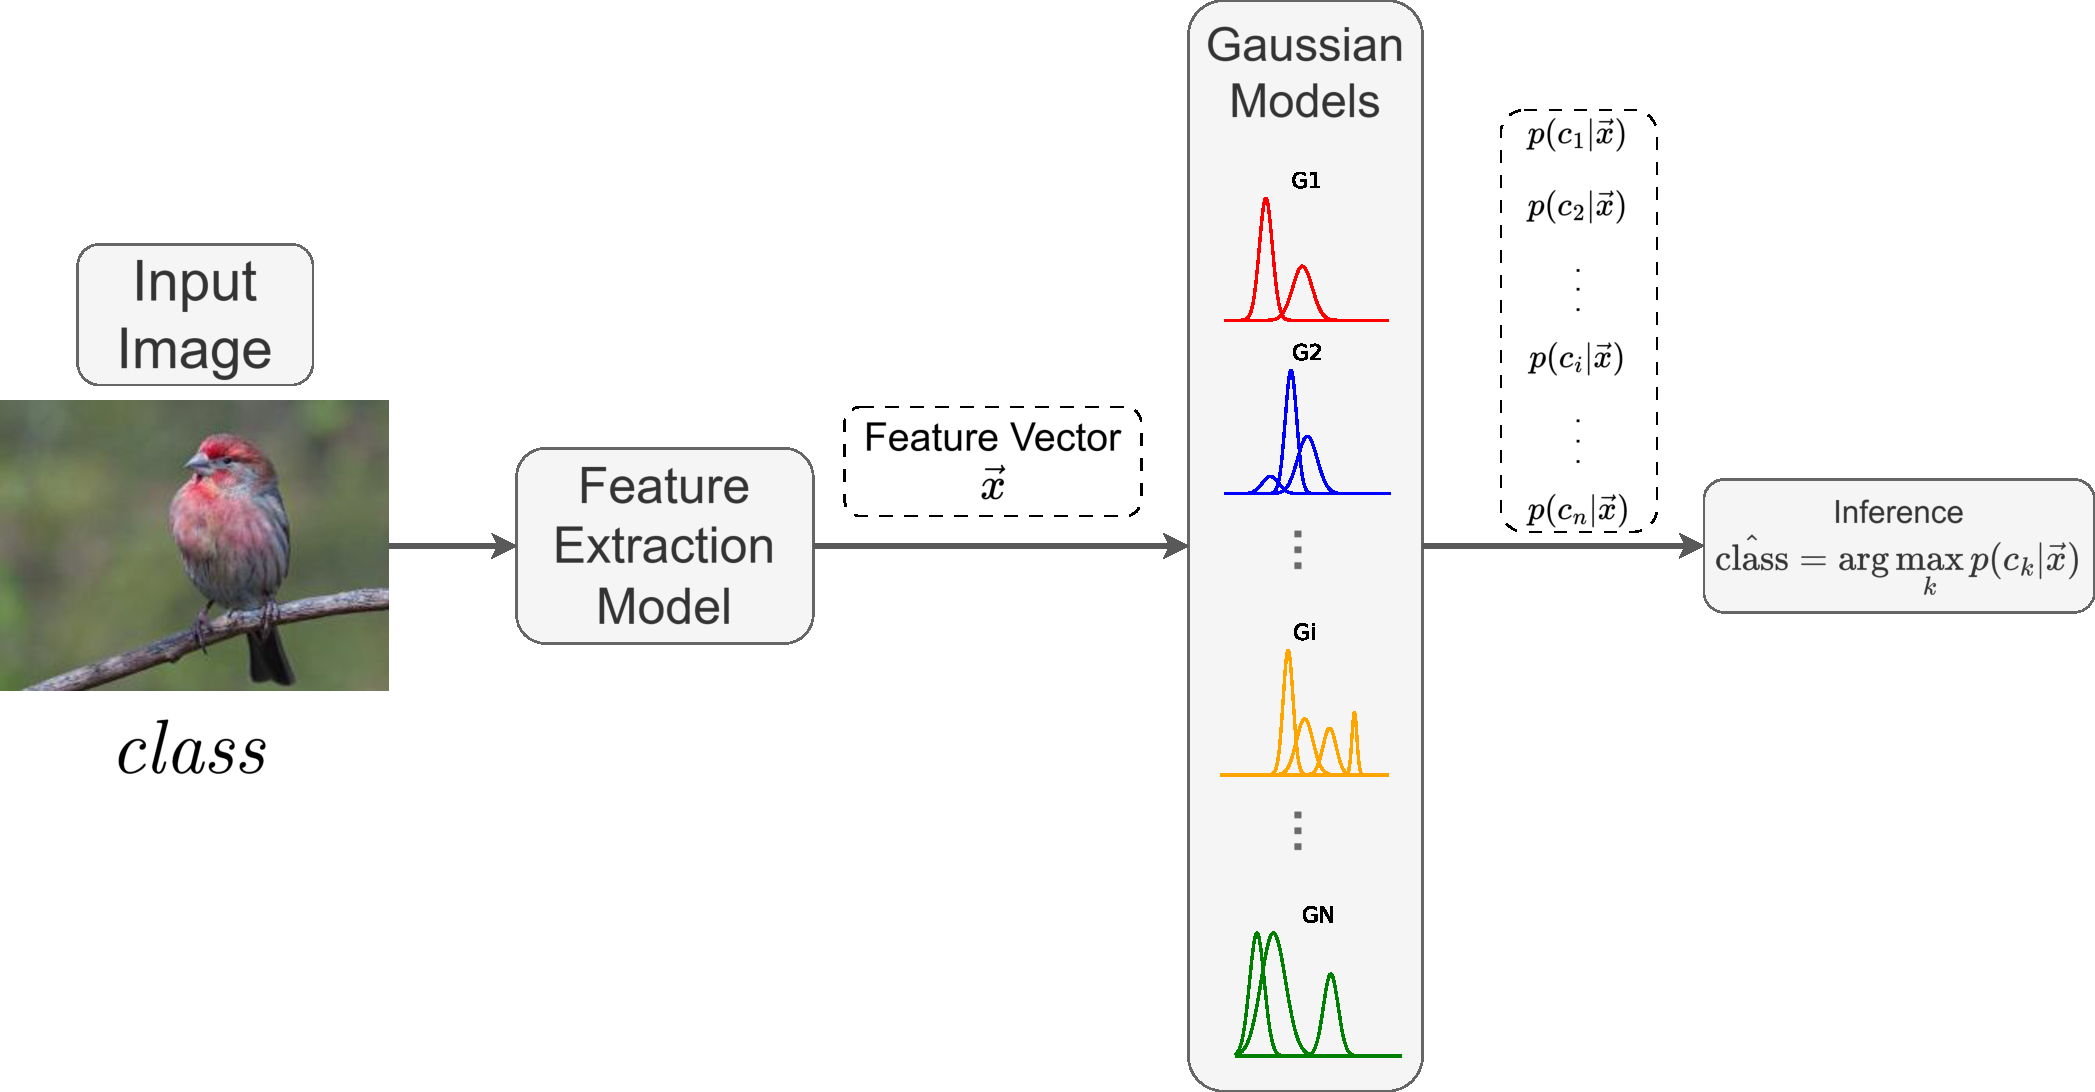
\includegraphics[width=0.7\textwidth]{imagenes/methodology/block_diagram_approach.pdf}
	\caption{Overview of the continual-learning framework: a frozen foundation model extracts features $\vec{x}$, classes are modeled independently as Gaussians ($G_k$) to allow dynamic registration without retraining, and inference predicts via Bayesian posterior maximization.}
	\label{fig:intro_overview}
\end{figure}

Gaussian class representations offer two key advantages that make them particularly well suited to this reframed problem. First, each class is modelled independently from the rest, so incorporating a new class amounts to estimating a small number of sufficient statistics (mean and covariance) and does not require any modification of the previously stored class models; this yields incremental updates that are exact and gradient-free, and that produce zero catastrophic forgetting by construction. Second, Gaussian models are compact: they encode each class in a few parameters that can be estimated from a modest sample budget and refined as new samples become available, without any storage of the underlying images. This second property, however, is far from trivial in practice: because the dimensionality $d$ of foundation-model embeddings (typically in the hundreds) is frequently comparable to, or larger than, the number of training samples $n_c$ available per class, the empirical covariance matrix is structurally rank-deficient whenever $n_c < d$. This thesis studies this small-sample regime in detail, evaluating a full spectrum of covariance parameterisations---from diagonal to full covariance matrices, including shared and shrinkage-based estimators.

Because the entire framework rests on the assumption that class-conditional features are approximately Gaussian, this assumption cannot be taken for granted: it must be empirically validated rather than merely postulated. This thesis therefore complements its architectural proposal with a rigorous statistical characterisation of the DINOv2 embedding space, combining moment-based diagnostics (skewness and excess kurtosis) with formal hypothesis tests---the D'Agostino--Pearson omnibus test \cite{dagostino1971omnibus,dagostino1973tests} for univariate normality and a diagonal adaptation of the Henze--Zirkler test \cite{henze1990class} for multivariate normality under severe rank deficiency. In parallel, the \emph{Bhattacharyya distance} is used to quantify inter-class separability and to establish a principled theoretical ceiling on the accuracy that any Gaussian classifier can achieve in a given feature space. This separability analysis is not merely descriptive: it is used throughout this thesis to identify, explain, and visualise the specific pairs of classes whose overlapping Gaussian distributions constitute the dominant source of classification error observed in this framework, as opposed to any degradation of previously learned representations.

\section{Hypothesis}

We hypothesize that the combination of an independent class-conditional Gaussian model and a frozen pre-trained feature extractor provides a robust framework for continual object classification. By enabling the addition of new classes without full-model retraining, this design eliminates catastrophic forgetting while maintaining a simple, compact architecture.

\section{General Objective}

The main objective of this thesis is to develop and to validate a continual learning framework for object classification using pre-trained foundation models and independent class-conditional Gaussian models as classifiers, with the purpose of enabling the incremental incorporation of new classes while preventing catastrophic forgetting.

\section{Specific Objectives}

For the purpose of fulfilling the general objective and verifying the hypothesis of this work, the following specific objectives are defined:

\begin{itemize}

	\item To assess the practical performance of the proposed framework across its own architectural variations—including different covariance-matrix estimators and Mixture-of-Gaussian variants—as well as against state-of-the-art baselines.
	
	\item To conduct an in-depth empirical analysis of the system's performance, measuring the effect of upstream backbone representations, progressive class expansion, confidence calibration metrics, and downstream computational cost.
	
	\item To statistically validate the underlying assumptions of the framework by analyzing the datasets representations within the feature extractor embedding space, specifically assessing the Gaussianity of class-conditional feature distributions, evaluating their spectral structure, and quantifying inter-class separability to identify the sources of residual classification error.

\end{itemize}

\section{Contributions}

The principal contributions of this thesis are the following:
\begin{enumerate}
	\item A gradient-free class-incremental learning framework that pairs a frozen DINOv2 backbone with independent, closed-form class-conditional Gaussian models, eliminating catastrophic forgetting by construction rather than by mitigation, together with a systematic evaluation of five covariance parameterisations (diagonal, full, hybrid, shared, and shrinkage-based) and their mixture-of-Gaussian extensions.
	\item A rigorous, multi-layered statistical validation of the Gaussianity assumption underlying the framework---combining moment-based diagnostics, the D'Agostino--Pearson omnibus test, and a diagonal adaptation of the Henze--Zirkler test for both univariate and multivariate normality under severe rank deficiency---that had not previously been carried out for foundation-model embedding spaces at this level of detail.
	\item A quantitative link between inter-class separability, measured via the pairwise Bhattacharyya distance, and the specific, named class pairs that account for the residual classification error of the proposed classifier, reframing that error as a property of the embedding space rather than of the classifier itself.
\end{enumerate}

\section{Thesis Structure}

The remainder of the document is organised as follows.

\paragraph{Chapter~\ref{ch:framework} -- Continual Learning and Foundation Models.} Covers the background needed to situate this work: the basics of artificial intelligence, machine learning, and deep learning applied to object classification, then continual learning itself, including catastrophic forgetting, the stability--plasticity dilemma, and the main families of existing solutions (rehearsal-, regularisation-, architecture-, and prompt-based methods, plus the classifier-adaptation and class-prototype approaches closest to what is proposed here). It closes with the Vision Transformer and the DINOv2 backbone used throughout this thesis.

\paragraph{Chapter~\ref{ch:gaussian_space} -- Statistical and Probabilistic Foundations of the Feature Space.} Lays out the mathematical and statistical tools the framework depends on: Bayesian classification and the Maximum A Posteriori rule, the Mixture-of-Gaussians model, and covariance estimation in the high-dimensional, small-sample regime typical of foundation-model embeddings. It also introduces the spectral tools used to describe the intrinsic dimensionality of the feature space, the tests used later to check the Gaussianity assumption, the Bhattacharyya and Euclidean separability metrics, and the confidence and calibration metrics used to judge how trustworthy the predictions are.

\paragraph{Chapter~\ref{methodology} -- Modelling Class Densities in a Frozen Feature Space.} Presents the proposed architecture in detail: a frozen encoder paired with independent, class-conditional Gaussian models updated in closed form, followed by the full family of covariance estimators evaluated in this thesis (diagonal, full, hybrid, OAS, Ledoit-Wolf, and shared covariance) and their Mixture-of-Gaussians extensions.

\paragraph{Chapter~\ref{ch:results} -- Experimental Results and Analysis.} Reports the experimental protocols and the resulting analysis: the datasets and evaluation protocol, calibration and covariance-estimator performance across benchmarks, accuracy as classes are added incrementally, inter-class separability and the specific class pairs behind the residual error, sensitivity to the choice of backbone, the spectral structure of the DINOv2 embedding space, and the empirical validation of the Gaussianity assumption. Across every one of these analyses, MOG4-Shared is evaluated alongside the rest of the estimators and identified as the strongest overall configuration once accuracy, calibration, and computational cost are all taken into account.

\paragraph{Chapter~\ref{ch:conclusion} -- Conclusion.} Draws together the central findings of the thesis, discusses the limitations of the current framework, and outlines directions for future work that follow directly from those limitations.

\chapter{Continual Learning and Foundation Models}
\label{ch:framework}

Continual Learning (CL) is the central problem this thesis addresses: how can a visual recognition system keep learning new object categories over time without catastrophically forgetting the ones it already knows? Answering this question rigorously, however, first requires a shared vocabulary. Before discussing what makes forgetting happen, what has been tried to prevent it, and how this thesis proposes to avoid it altogether, we must establish the fundamental principles of Artificial Intelligence, Machine Learning, and Deep Learning on which every subsequent argument rests, closing this introductory background with Computer Vision and its Object Classification task---the specific setting, including a first, necessarily brief, encounter with the Transformer architecture, in which the Continual Learning problem studied in this thesis is framed.

With this vocabulary in place, we return to Continual Learning and examine it in the depth the central problem of this thesis demands: the challenge of catastrophic forgetting, the stability--plasticity dilemma it creates, the main paradigms used to formulate it, and a review of the state-of-the-art mitigation strategies that provide both a performance baseline and the motivation for this thesis. This review then gives way, fluidly, to the representation-learning backbone that the proposed framework builds upon: Vision Transformers and, in particular, the self-supervised DINOv2 architecture.

\section{Artificial Intelligence and Machine Learning}
\label{sec:framework:ai_ml}

Artificial Intelligence (AI) is a broad field of computer science dedicated to creating systems capable of performing tasks that typically require human intelligence, such as learning, reasoning, perception, and language understanding \cite{RussellNorvig}. Within this domain, Machine Learning (ML) focuses on developing algorithms that allow computers to learn patterns from data without explicit programming. ML systems are generally categorized into three paradigms: Supervised Learning, Unsupervised Learning, and Reinforcement Learning \cite{Bishop2006}.

First, in \textbf{Supervised Learning}, the model learns a mapping from input variables $\mathbf{x}$ to output variables $y$ based on a labeled dataset $\mathcal{D} = \{(\mathbf{x}_i, y_i)\}_{i=1}^N$. The objective is to minimize a loss function that penalizes the discrepancy between the predicted output and the ground truth. This paradigm is typically divided into Classification, where the output is a discrete category, and Regression, where the output is a continuous value.

Second, \textbf{Unsupervised Learning} deals with unlabeled data $\mathcal{D} = \{\mathbf{x}_i\}_{i=1}^N$. Instead of predicting a target, the goal is to discover the underlying structure or distribution of the data. Common tasks include Clustering, which groups similar data points (e.g., K-Means or Gaussian Mixture Models), and Dimensionality Reduction, which projects high-dimensional data into a lower-dimensional space while preserving essential information (e.g., PCA or t-SNE).

Finally, \textbf{Reinforcement Learning} is based on an agent interacting with an environment to maximize a cumulative reward. Unlike supervised learning, the agent is not told which actions to take but must discover them through trial and error. This process is often modeled as a Markov Decision Process (MDP) \cite{Sutton2018}, where the agent transitions between states based on actions, receiving feedback in the form of numerical rewards. 
The focus is on finding an optimal policy that maximizes long-term return, a process that requires balancing exploration (trying new actions) and exploitation (capitalizing on known high-reward actions) during learning.
 %The focus is on finding an optimal policy that balances exploration (trying new actions) and exploitation (using known high-reward actions).

\subsection{Deep Learning}

In traditional Machine Learning, the feature extraction step is a manual process where a human expert must identify and define the most relevant characteristics (such as the shape or edges of the car) before passing them to a classification algorithm. In contrast, as shown in figure \ref{fig:deep_learning}, Deep Learning utilizes neural networks to automate this process; the model performs both feature extraction and classification simultaneously, learning to identify complex patterns directly from the input data without human intervention.

This shift allows Deep Learning to handle much more complex, high-dimensional data, though it typically requires significantly larger datasets and more computational power to be effective. While traditional Machine Learning depends on the quality of hand-crafted features, Deep Learning architectures—like multi-layered neural networks—are designed to build hierarchical representations of data, progressively moving from low-level pixels to high-level object concepts.

\begin{figure}[htb]
	\centering
	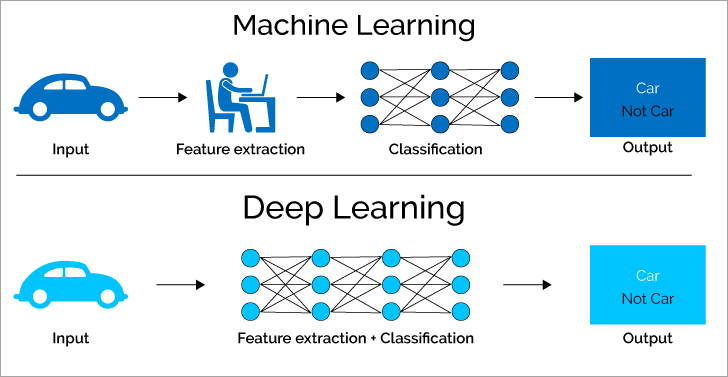
\includegraphics[width=0.7\textwidth]{imagenes/marco/deep.png}
	\caption{Machine Learning and Deep Learning Strategies. Image taken from \cite{deep}.}
	\label{fig:deep_learning}
\end{figure}

\subsection{Computer Vision}
\label{sec:framework:cv}

Computer Vision is the interdisciplinary field that enables computers to gain high-level understanding from digital images or videos, effectively automating tasks performed by the human visual system \cite{Szeliski2010}. While Convolutional Neural Networks (CNNs) \cite{CNN} historically dominated this field, the Transformer architecture---originally developed for Natural Language Processing---has revolutionized visual recognition through the self-attention mechanism \cite{AttentionIsAllYouNeed}.

Among the many tasks studied in Computer Vision, \textbf{Object Classification} is one of the most fundamental: it consists of assigning a single categorical label to an entire input image, and it serves as the primary benchmark for evaluating the representative power of visual models \cite{Krizhevsky2012}. This task is the setting adopted throughout this thesis: the Continual Learning problem discussed next is studied specifically as a sequence of object classification tasks, in which the model must progressively learn to assign incoming images to a growing set of object categories.

Having established this general background in Artificial Intelligence, Machine Learning, Deep Learning, and Computer Vision---including a first glimpse of the Transformer architecture that will reappear in depth later in this chapter---we now turn to the specific paradigm around which this thesis is organized: Continual Learning, studied here within the object classification setting.

\section{Continual Learning}
\label{sec:framework:cl}

Continual Learning (CL), also known as lifelong learning, addresses the problem of progressively acquiring knowledge from non-stationary data streams over time. In object classification, this setup presents data as a sequence of disjoint tasks, where each task introduces a new set of object categories. The primary challenge is enabling a model to learn these novel categories incrementally without degrading its classification performance on previously acquired ones. As illustrated in Figure \ref{fig:task_time}, a \textbf{task} in this context a is 
defined as a specific learning session or split—such as Task A, B, or C—each introducing distinct class-conditional data distributions, symbolized by the varying shapes (e.g., circles vs. hearts) above the task labels.

% is defined as a specific learning experience or dataset –such as Task A, B, or C. Each task is potentially characterized by unique data distributions or objectives, as symbolized by the varying shapes (e.g., circles vs. hearts) above the task labels.

Unlike conventional training approaches that rely on a fixed dataset and a stationary environment, CL emphasizes the arrival of these tasks at distinct intervals along the \textbf{time} axis. This sequential arrival requires the model to be inherently non-stationary, adapting its internal representations as environments evolve. The primary challenge in this paradigm lies in the ongoing integration of new information from a current task (e.g., Task B) while simultaneously preserving the knowledge previously acquired from Task A.

\begin{figure}[htb]
	\centering
	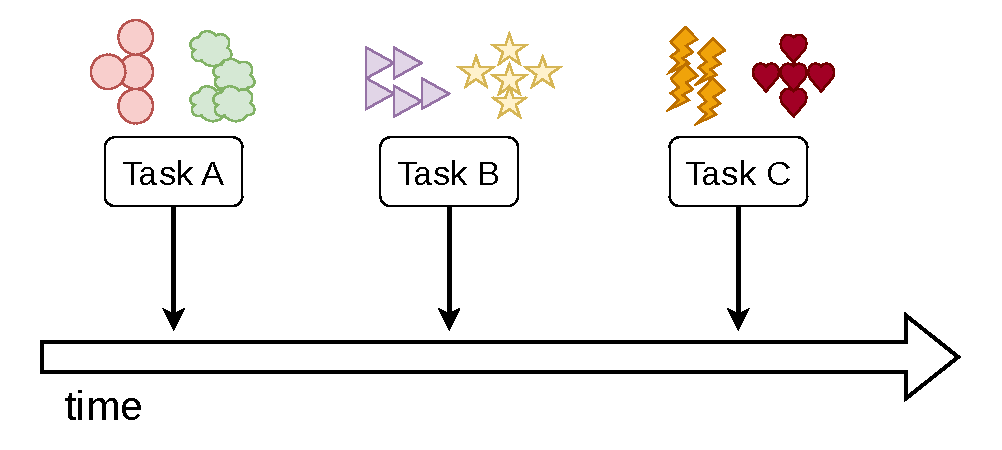
\includegraphics[width=0.75\textwidth]{imagenes/marco/Adaptation.pdf}
	\caption{A sequential task arrival model for Continual Learning, depicting the transition from Task A to Task C over time, where each task represents a unique set of features or data distributions.}
	\label{fig:task_time}
\end{figure}

Without specific architectural or algorithmic safeguards, this sequential learning process inevitably triggers \textbf{catastrophic forgetting} \cite{CL}. This phenomenon occurs when the assimilation of new knowledge leads to the degradation or total loss of prior learning. As illustrated in Figure \ref{fig:catastrophic_forgetting}, the dilemma of forgetting becomes apparent when a \textit{New Object Class} is introduced to an existing classifier, forcing a choice between two traditional but flawed strategies:

\begin{itemize}
	\item \textbf{Fine-Tuning:} Updating the model using only the current task data is computationally efficient but leads directly to catastrophic forgetting \cite{CL}. Because the optimization process focuses solely on the new objective, the internal representations associated with previously learned classes are overwritten, causing the model to lose its original predictive capabilities.

	\item \textbf{Retraining from Scratch:} While joint training on the full historical dataset ($\mathcal{D}_{old} \cup \mathcal{D}_{new}$) technically prevents forgetting, it faces two significant hurdles. First is the issue of \textbf{Data Privacy and Availability}: in many real-world scenarios, the original data $\mathcal{D}_{old}$ is often deleted or inaccessible due to privacy regulations. Second is the \textbf{Computational Bottleneck}: as the system's lifespan increases, the cumulative dataset grows, making the energy and time required to retrain the model unsustainable in continuously evolving environments.
\end{itemize}

\begin{figure}[htb]
	\centering
	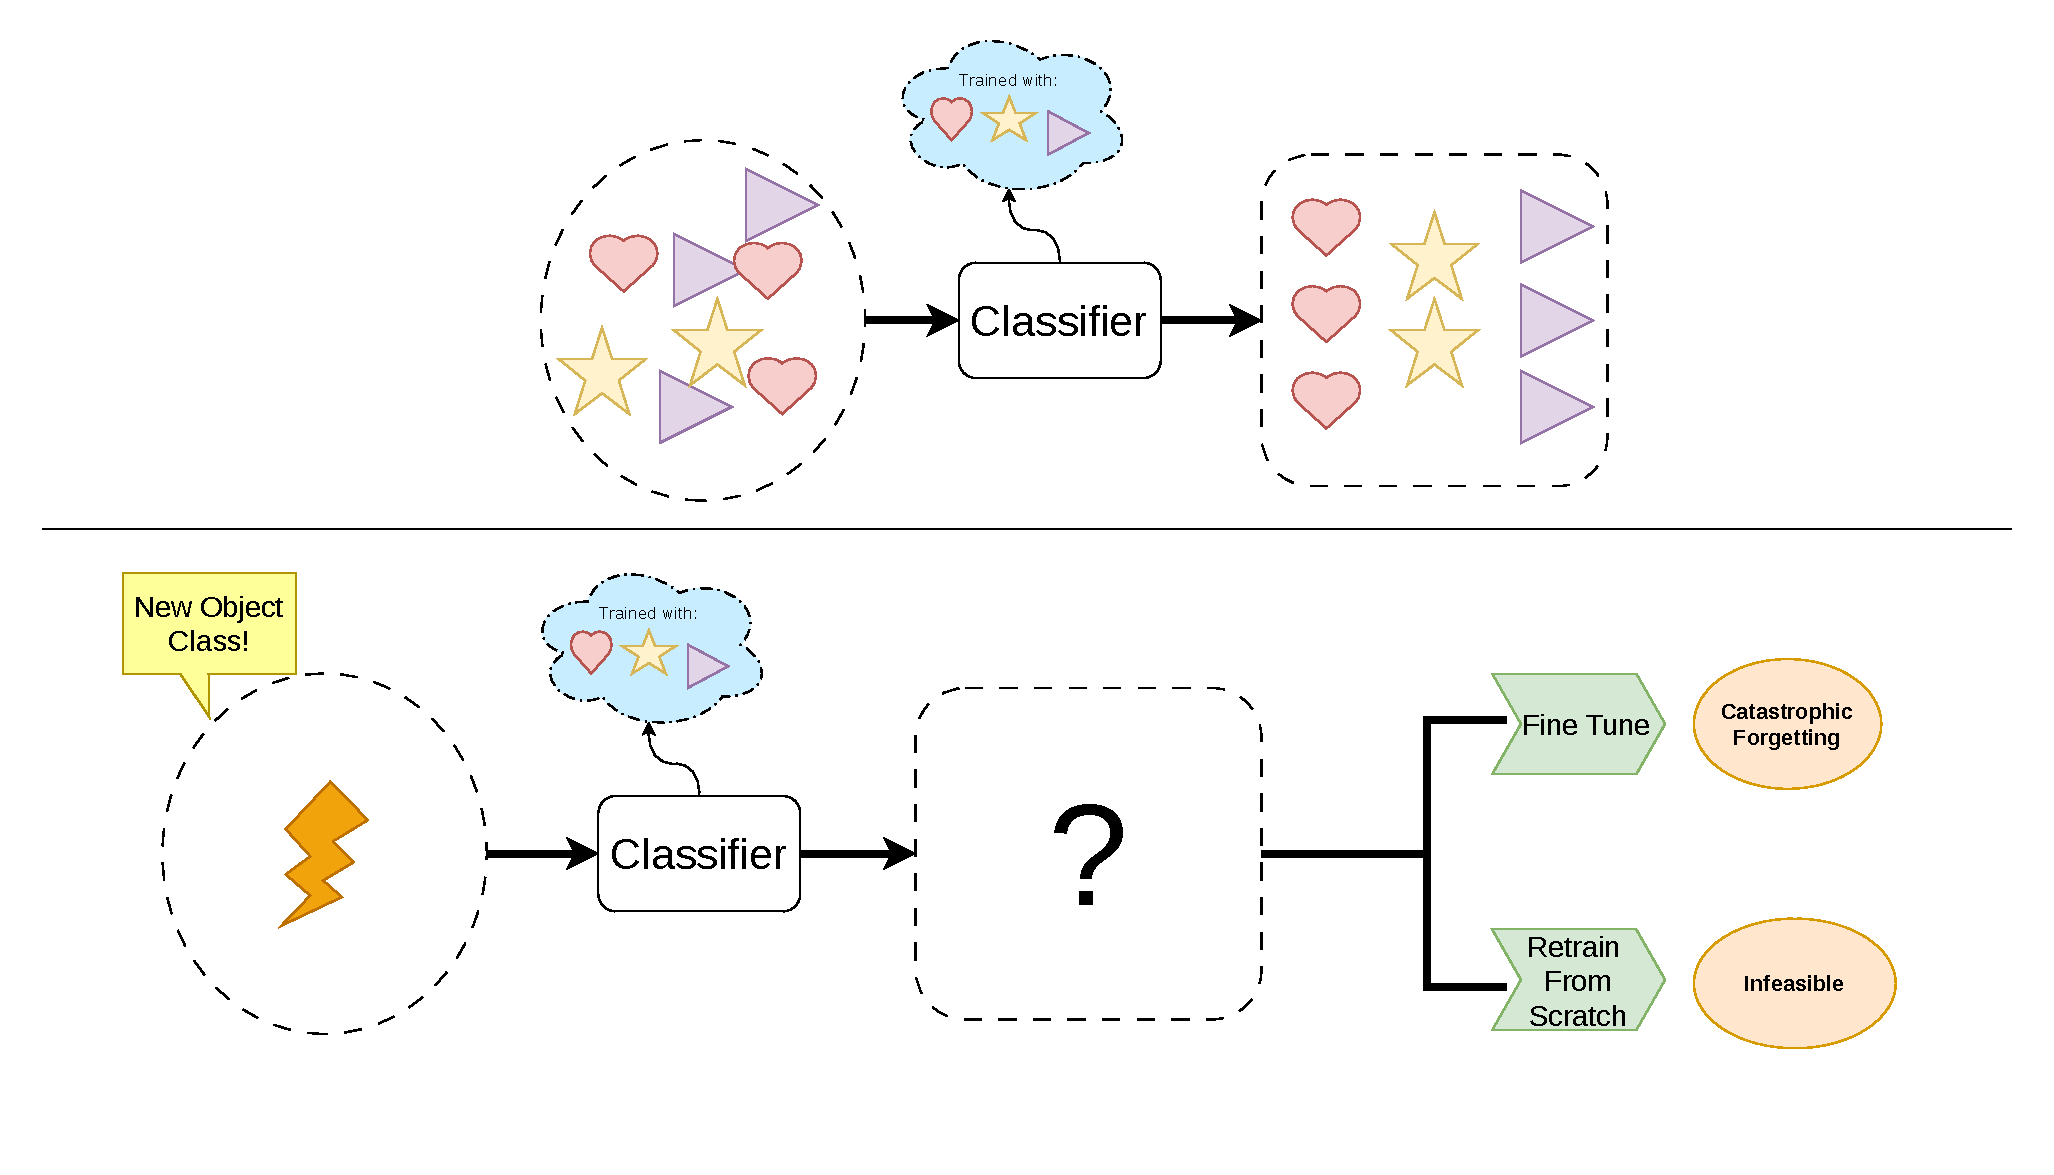
\includegraphics[width=0.8\textwidth]{imagenes/marco/Catastrophic_forgetting.pdf}
	\caption{Standard Object Classifier comparison. The upper path shows standard inference, while the lower path illustrates the dilemma when a new class is introduced: the trade-off between catastrophic forgetting via fine-tuning and the infeasibility of retraining from scratch.}
	\label{fig:catastrophic_forgetting}
\end{figure}

\subsection{Stability and Plasticity}
A central concept in continual learning is the balance between stability and plasticity. \textbf{Stability} emphasizes preserving the parameters and representations that are crucial for retaining old knowledge \cite{API}. \textbf{Plasticity}, in contrast, refers to the ability of a model to adapt rapidly to new information, ensuring that it can effectively learn novel tasks. Achieving an appropriate equilibrium between these two properties is known as the \textbf{stability–plasticity dilemma} \cite{CL}.

\subsection{Main Paradigms}
As shown in Figure \ref{fig:task_vs_class}, two principal paradigms define how continual learning problems are formulated. \textbf{Task-incremental learning (Task-IL)} assumes that the task identity is available during inference, allowing for task-specific components to be isolated \cite{task_il}. \textbf{Class-incremental learning (Class-IL)}, on the other hand, does not provide the task identity at test time, requiring the model to distinguish between all classes seen across all tasks simultaneously \cite{masana_class_il}.

\begin{figure}[htb]
	\centering
	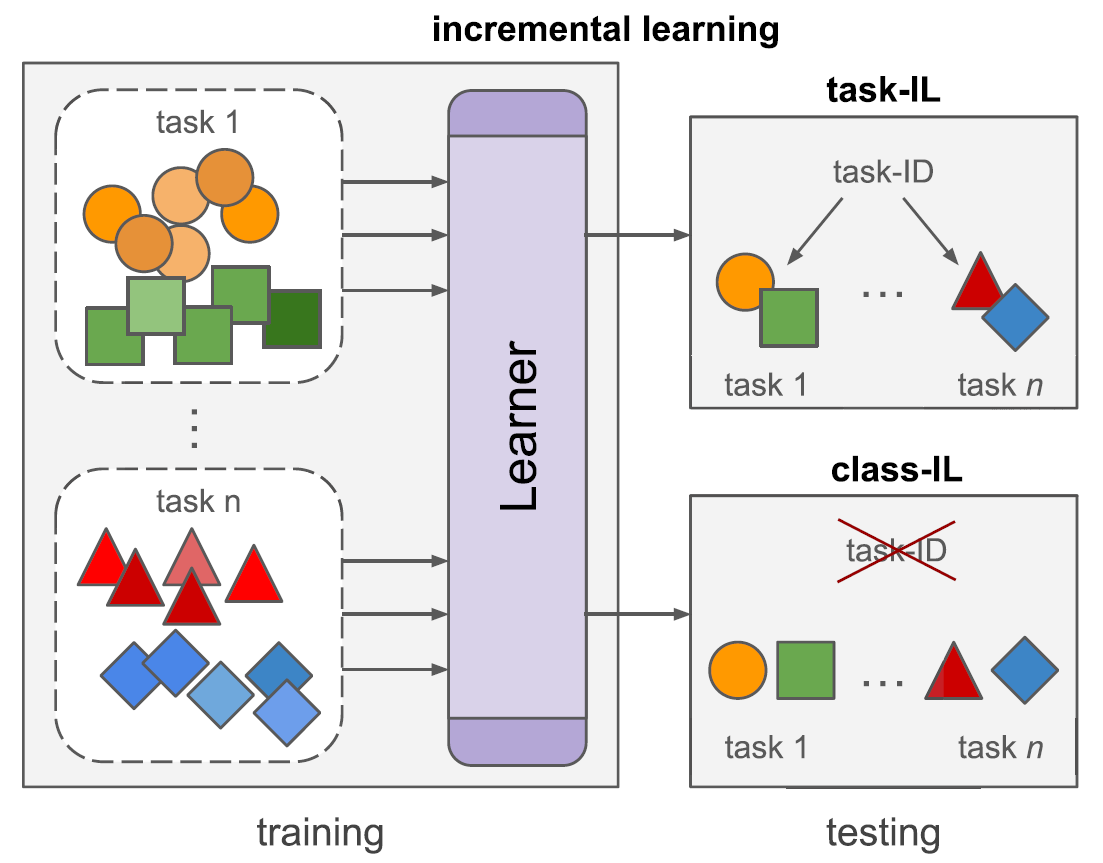
\includegraphics[width=0.5\textwidth]{imagenes/marco/CI_learning_survey_fig1.png}
	\caption{Class and Task Incremental Learning. Image taken from \cite{masana_class_il}.}
	\label{fig:task_vs_class}
\end{figure}

\subsection{Related Work in Continual Learning}

To address the stability–plasticity dilemma, we categorize continual learning strategies into five broad approaches: rehearsal, regularization, architecture-based methods, representation and prompt-based tuning, and classifier adaptation over frozen representations. Classifier adaptation—both its discriminative and analytic, prototype-based variants—is the approach most directly comparable to the framework proposed in this thesis, so it's the one we treat as the closest point of reference.

\subsubsection{Rehearsal Methods}

Rehearsal-based methods target the most direct cause of catastrophic forgetting: once training on a new task starts, there is no gradient signal left telling the model anything about what it already learned. So they mix a handful of past examples into the current task's training data—sometimes these are just the original images sitting in a small buffer, sometimes they are synthetic examples that a separate generator recreates on the fly instead of storing anything real—keeping the model reminded of the old classes even while it is busy learning the new ones. The real design question is what to keep and how to use it efficiently, since a memory buffer with no limits would defeat the whole point of a learner that has to run with limited memory and storage.

\begin{itemize}
	\item \textbf{Experience Replay (ER)} \cite{Chaudhry2019ContinualLW} is the simplest instantiation of this idea: a small episodic memory buffer retains a random or reservoir-sampled subset of past examples, which are interleaved with the current task's mini-batches so that every gradient step still receives some supervision on old classes. Its simplicity makes it a common and surprisingly strong baseline, but its effectiveness scales with buffer size, and the fixed capacity inevitably biases the retained sample toward whichever selection heuristic is used.
	
	\item \textbf{Average Gradient Episodic Memory (A-GEM)} \cite{agem} reframes the buffer's role from a source of additional gradient signal to a constraint on the optimisation trajectory itself: rather than training jointly on old and new samples, it projects the current task's gradient so that it does not increase the loss computed on a reference batch drawn from the buffer, which is considerably cheaper than the original GEM formulation while retaining most of its forgetting-mitigation benefits.
	
	\item \textbf{Dark Experience Replay (DER)} \cite{buzzega2020darkexperiencegeneralcontinual} enriches the stored exemplars with the network's own past output logits rather than only their hard labels, and distils this ``dark knowledge''---the full soft-label distribution encoding inter-class similarity structure learned at the time of storage---back into the current model. This provides a denser training signal per replayed sample than label-only rehearsal, at the cost of needing to persist and periodically re-align these logits with a model that is continually changing.
	
	\item \textbf{Generative Replay} \cite{generative_features} sidesteps the need to store raw exemplars altogether by training a generative model (or, in feature-space variants, a feature synthesiser) to reproduce samples of previously seen classes on demand. This removes the raw-data privacy liability of exemplar buffers, but transfers the difficulty elsewhere: the generator itself must be continually updated without forgetting, and any drift in the quality of its synthetic samples directly corrupts the rehearsal signal for old classes.
\end{itemize}

Across all four variants, the shared limitation is structural rather than incidental: rehearsal methods require either persistent storage of raw or compressed past data, or a generative model that is itself subject to the same forgetting dynamics it is meant to prevent, and their forgetting-mitigation quality degrades gracefully but monotonically as the buffer-to-task-count ratio shrinks over a long task stream.

\subsubsection{Regularization Methods}

Rather than revisiting old data, regularization-based methods attempt to identify, at the parameter level, which weights of the network are responsible for previously learned behaviour, and then constrain how much those specific weights are allowed to move while training on new tasks. The stability--plasticity trade-off is therefore made explicit as a per-parameter penalty: important parameters are frozen or heavily penalized for movement, while the remaining capacity of the network is left free to absorb new information.

\begin{itemize}
	\item \textbf{Elastic Weight Consolidation (EWC)} \cite{Kirkpatrick_2017} estimates parameter importance using the diagonal of the Fisher Information Matrix computed on each task, then adds a quadratic penalty to the loss that discourages movement away from the previous task's optimum in proportion to that importance. The approach is elegant and grounded in a Bayesian interpretation of sequential posterior updates, but the diagonal Fisher approximation ignores parameter interactions, and the accumulated quadratic penalties from many tasks can over-constrain the network, progressively eroding its plasticity.
	\item \textbf{Synaptic Intelligence (SI)} \cite{zenke2017continuallearningsynapticintelligence} computes an online, per-synapse importance measure by accumulating each parameter's contribution to the reduction of the loss along the entire training trajectory of a task, avoiding the need for a separate importance-estimation pass after each task and making the method considerably cheaper than EWC in practice, though it inherits a similar long-horizon rigidity problem.
	\item \textbf{Learning Without Forgetting (LwF)} \cite{li2017learningforgetting} regularises the network's function rather than its parameters directly: before training on a new task, the previous model's predictions on the new task's inputs are recorded, and a knowledge-distillation loss then penalises deviations of the updated model's outputs from these recorded soft targets. This makes LwF architecture-agnostic and exemplar-free, but its effectiveness depends on the new task's inputs being informative enough to anchor the old decision boundaries, which becomes unreliable under large domain shifts between tasks.
	\item \textbf{Adaptive Plasticity Improvement (API)} \cite{API} takes a more geometric view, using Dual Gradient Projection Memory (Dual-GPM) to identify the subspaces of parameter (or gradient) space that were important for previous tasks and enforcing that new updates proceed in directions orthogonal to them. This directly targets the stability side of the dilemma by construction, but the number of protected subspaces necessarily grows with the number of tasks, gradually shrinking the remaining free subspace available for future plasticity.
\end{itemize}

The common thread across this family is that importance estimates---whether Fisher-based, synaptic, distillation-based, or subspace-based---are necessarily approximate and computed with respect to the tasks seen so far; as the task stream lengthens, the accumulated constraints compete for a fixed parameter budget, and all four methods must trade off increasingly aggressive stability against a shrinking capacity for plasticity.

\subsubsection{Architecture-based Methods}
A third family sidesteps the stability--plasticity trade-off at the parameter level altogether by modifying the network's structure itself, either by isolating the sub-networks responsible for each task or by physically growing the network's capacity as new tasks arrive.
\begin{itemize}
	\item \textbf{Parameter Isolation} \cite{10.5555/3454287.3455512} identifies and freezes the specific parameters or sub-networks important for previous tasks---typically through pruning or learned gradient masks---so that only a designated, disjoint subset of weights remains trainable for the current task. This offers a strong, structural guarantee against forgetting for the frozen parameters, but the available free capacity shrinks monotonically as more tasks are isolated, and, in many instantiations, recovering which sub-network to use at inference time requires knowledge of the task identity.
	
	\item \textbf{Dynamic Expansion} methods take a more literal approach: instead of freezing parts of a fixed-size network, they let the network itself grow. DER~\cite{Yan2021DERDE} (Dynamically Expandable Representation, not to be confused with Dark Experience Replay above) keeps everything learned so far completely frozen and, for each new task, bolts on a brand-new trainable branch next to it; the outputs of all branches get concatenated into one large ``super-feature'', and a pruning step afterward trims away whatever redundant channels that new branch didn't really need. DEN~\cite{Yoon2017LifelongLW} (Dynamically Expandable Networks) is more conservative: rather than always adding a new branch, it first tries to fit the new task using the capacity that's already there, and only grows the network—adding new units—when the training loss shows that existing capacity genuinely isn't enough. Both approaches guarantee that old sub-networks remain untouched and hence immune to forgetting by construction, but at the cost of a parameter count, and consequently a memory and computational footprint, that grows over the lifetime of the system---an increasingly serious limitation for long task streams.
\end{itemize}

Whether through isolation or expansion, architecture-based methods trade the risk of interference for an explicit, often unbounded, growth in model complexity, and frequently still require task identity at inference to route each input to the correct sub-network---a requirement that is unavailable in the class-incremental setting studied throughout this thesis.

\subsubsection{Representation and Prompt-based Methods}
The rise of foundation models (e.g., ViTs, described in detail in Section~\ref{sec:framework:foundation_models}) opened up a different strategy altogether: instead of touching the backbone's weights at all, these methods leave it completely frozen and confine all task-specific learning to a small set of extra parameters called \emph{prompts}. Concretely, a prompt is a short sequence of learnable embedding vectors that gets prepended to, or otherwise inserted into, the sequence of patch tokens the Transformer already processes for a given image; the backbone treats these vectors exactly as it would treat any other token, so they never change a single one of the network's own weights, but they do change what the network attends to and, through that, the features it eventually outputs for that image. Since the backbone itself never changes, forgetting at the representation level cannot happen by construction; the real challenge shifts to designing prompts expressive enough to adapt the frozen features to each task, without ever telling the model which task it is currently looking at.
\begin{itemize}
	\item \textbf{Learning to Prompt (L2P)} \cite{wang2022learning} keeps a pool of learnable prompts and, for each input, picks out and combines the ones that best match it: every prompt has an associated key vector, and the input's own embedding is compared against these keys to decide which prompts to use. Because this selection is done per input rather than per task, the same shared pool can serve every task without ever needing to know which one is currently active; the trade-off is that the whole approach now depends on that matching step working correctly, and a wrong match sends the input to prompts meant for entirely different content.
	\item \textbf{Dual Prompt} \cite{wang2022dualprompt} builds on this by splitting the prompt pool into two clearly different roles: a set of fixed, shared \emph{General} prompts that capture knowledge common to all tasks, and task-specific \emph{Expert} prompts that specialize the representation for the classes belonging to one particular task. This division gives a better balance between remembering old tasks and learning new ones than L2P's single undifferentiated pool, though it still needs the same kind of key-based matching to pick out the right Expert prompt at inference time.
	\item \textbf{CODA-Prompt} \cite{Smith_2023_CVPR} does away with that hard, similarity-based matching step entirely. Instead of picking a discrete subset of prompts, it combines all of them through an attention-weighted average, so the whole prompting mechanism can be trained end-to-end together with the classifier, rather than depending on a separately tuned matching heuristic.
	\item \textbf{Advanced Prompting} extensions carry this same idea into more efficient and distributed settings: \textbf{InFLoRA} \cite{liang2024inflora} and \textbf{DOLFIN} \cite{dolfin} apply low-rank adaptation and distributed training, respectively, to cut down the parameter cost of maintaining a prompt pool, while \textbf{APT} \cite{Chen_2025_ICCV} skips prompt selection altogether by injecting key-value tokens directly into the transformer's attention layers, which also reduces the computational cost at inference time.
\end{itemize}

Across this family, freezing the backbone rules out representation-level forgetting almost by definition, but everything then depends on how well the prompt-selection mechanism works. That mechanism brings its own extra parameters and its own training difficulties, and because prompts are usually learned by backpropagating through the frozen backbone, it also adds a computational cost per task that the purely analytic methods discussed next manage to avoid entirely.

\subsubsection{Classifier Adaptation on Frozen Representations}
A complementary line of work also keeps the feature extractor frozen, just like prompt-based methods do, but skips learnable prompts entirely: the frozen embedding is simply taken as-is, and all the adaptation happens in a discriminative or metric-based classifier built directly on top of it, with no backpropagation through the backbone at all.

\begin{itemize}
	\item \textbf{SLCA} \cite{zhang2023slca} proposes a slow learner with classifier alignment for continual learning on pre-trained models: the backbone is fine-tuned with a substantially reduced learning rate to preserve its pre-trained generality, while a separate classifier head is periodically re-aligned to correct for the resulting representation drift, enabling efficient incremental learning without the full instability of end-to-end fine-tuning.
	\item \textbf{ACIL} \cite{zhuang2022acil} treats incremental learning analytically: following an initial base phase where the CNN backbone is trained via backpropagation and subsequently frozen, it projects the extracted embeddings into a higher-dimensional space via a randomized feature expansion layer with non-linear activations. A linear classifier is then updated over these expanded features using recursive regularized least-squares, which provably reproduces the joint-training closed-form solution over all observed classes without revisiting past data, ensuring absolute memorization and data privacy without exemplar storage.
	\item \textbf{FeCAM} \cite{goswami2024fecam} exploits the heterogeneity of class distributions in this exemplar-free setting by replacing the Euclidean or purely linear decision rules of the methods above with a Mahalanobis-distance-based classifier, explicitly accounting for the fact that different classes occupy differently shaped regions of the frozen embedding space.
\end{itemize}

Because the backbone is never updated, none of these methods suffers representation-level forgetting, and---unlike prompt-based methods---none of them requires backpropagation at all during incremental updates; the price is that their classifiers rely on comparatively simple statistical or geometric assumptions about the embedding space, which the next family of methods begins to make explicit.

\subsubsection{Class Prototype and Analytic Classifier Methods}
\label{sec:marco:prototype_methods}
A closely related family of methods represents each class through distances to class prototypes (first-order information), sometimes complemented by second-order statistics, and is the family most directly comparable to the framework proposed in this thesis.
\begin{itemize}
	\item \textbf{SimpleCIL} \cite{janson2022simple} performs first-session adaptation by applying parameter-efficient fine-tuning (PEFT) to the backbone only during the initial task, after which the backbone is frozen for the remainder of the stream and class prototypes are computed simply as the mean embedding of the samples belonging to each class. Its simplicity and strong empirical performance on foundation-model embeddings established that even a purely first-order, distance-to-mean classifier can be a remarkably strong baseline once the backbone is sufficiently general.
	\item \textbf{RanPAC} \cite{mcdonnell2023ranpac} improves upon this prototype-based scheme by first applying a fixed random projection followed by a non-linear activation, lifting the features into a higher-dimensional space in which classes become more linearly separable by construction (a random-feature approximation of a kernel expansion), and then accumulating second-order information through a shared, incrementally updated Gram matrix across all classes rather than per-class covariances.
	\item \textbf{FeTrIL} \cite{petit2023fetril} stores only the centroid representation of each past class rather than any raw exemplars or full covariance matrices. When a new task arrives, features of the new classes are geometrically shifted toward past class regions using the difference between past and new class centroids; the resulting pseudo-features are then used alongside real new-class features to train a linear classifier incrementally.
	\item \textbf{FeCAM} \cite{goswami2024fecam}, already introduced above, is more naturally placed in this family for its second-order treatment: it explores Mahalanobis distances instead of typical Euclidean distances, applying a Tukey power-ladder transformation to correct feature skewness before normalising each class covariance so that its diagonal entries equal one, making Mahalanobis distances comparable across classes despite never validating that the underlying feature distributions justify a Gaussian, Mahalanobis-based treatment in the first place.
\end{itemize}

Across this family, representing a class through its prototype brings real efficiency, but that efficiency comes at a representational cost: first-order methods such as SimpleCIL and FeTrIL reduce a class to a single point in the embedding space, discarding the covariance information that describes how the class's features actually spread around that point, while RanPAC and FeCAM recover richer, second-order structure without a principled probabilistic model to justify the specific distance or normalization they apply, and neither checks whether treating class covariance this way is consistent with how the class distributions actually look.

\paragraph{Summary of Limitations.}
Across all five families, the same pattern recurs: each avoids one part of the stability--plasticity trade-off only by pushing its cost elsewhere---onto a growing memory or generator, a hardening set of importance constraints, an unbounded architecture, a fragile prompt-selection mechanism, or a classifier built on first-order or heuristic statistics rather than a proper probabilistic model. None of them checks whether the Gaussian assumption behind their distance metrics actually holds in the embedding space, or ties inter-class separability directly to the accuracy that can realistically be expected.

These limitations motivate a framework that (i) avoids exemplar storage, generator training, growing architectures, and backpropagation altogether by keeping the backbone entirely frozen and updating only closed-form sufficient statistics; (ii) models each class with a full, properly normalized multivariate Gaussian density rather than a heuristic distance metric, restoring a direct probabilistic and generative interpretation; and (iii) explicitly and statistically validates the Gaussian assumption on which this generative model rests, rather than simply asserting it.

\section{Foundation Models}
\label{sec:framework:foundation_models}

Having introduced Continual Learning as the central topic of this thesis, we now turn to a different piece of background this framework depends on: foundation models, the broader category of models the representation-learning backbone belongs to, and in particular Vision Transformers and the DINOv2 architecture used as the frozen feature extractor throughout this work. Before getting into the details of these two architectures, though, it is worth stepping back and asking what a foundation model actually is, and why a model of that kind is exactly what a frozen, exemplar-free continual learner needs.

\subsection{The Foundation Model Paradigm}
\label{sec:framework:foundation_paradigm}

A \textbf{foundation model} is best understood by the role it plays rather than by any single architecture: it is a large-scale model pre-trained on vast quantities of data and subsequently adaptable to a wide range of downstream tasks with comparatively little task-specific effort. The term itself was coined by researchers at the Stanford Institute for Human-Centered AI precisely to capture this role: these models are not built for one job, but act as a common technological base on top of which many specialised applications are eventually constructed \cite{bommasani2021opportunities}.

What really changes compared to a traditional machine learning pipeline is where the effort goes. Instead of training a task-specific architecture from scratch on a carefully generated by hand dataset, foundation models split the work into two clearly separated phases. The first, \emph{pre-training at scale}, exposes the network to huge amounts of data---web text, image collections, or multimodal data, depending on the domain---often, though not always, using self-supervised objectives such as predicting masked tokens or learning contrastive or self-distilled representations, which keep manual annotation to a minimum. The network just picks up rich, general-purpose structure about whatever domain it is trained on. The second phase, \emph{downstream adaptation}, takes this pre-trained network---frozen entirely or updated only slightly---and repurposes it for a specific target task through comparatively lightweight means: linear probing, parameter-efficient fine-tuning, or even zero-shot prompting, without ever retraining the backbone from scratch.


This two-phase recipe works across pretty much any type of data, largely because most foundation models, whatever they are trained on, share the same underlying architecture: the Transformer. In language, this gives rise to models such as GPT, Llama, and Gemini, which learn how words and phrases relate to each other well enough to support reasoning, translation, and text generation. In vision, the same recipe produces Vision Transformers and segmentation models such as the Segment Anything Model (SAM) \cite{kirillov2023segment}, which build detailed spatial and visual representations that carry over to detection, segmentation, and classification tasks. And across different types of data at once, systems such as CLIP or GPT-4o map images, text, and audio into a single shared space, letting them reason across all of them together.

\subsection{Vision Transformers}

Within this landscape, Vision Transformers are the specific architecture this thesis builds on. As introduced in Section~\ref{sec:framework:cv}, the Transformer---originally developed for Natural Language Processing---changed visual recognition by relying on self-attention \cite{AttentionIsAllYouNeed}, a mechanism that lets every element of the input attend directly to every other element, and this challenged the long-standing dominance of Convolutional Neural Networks (CNNs) \cite{CNN} in Computer Vision.

A Vision Transformer (ViT) adapts this architecture to images by treating them as a sequence of discrete tokens, the same kind of input a Transformer would otherwise expect from a sentence of words. As illustrated in Figure \ref{fig:ViTArchitecture}, this is done through a specific pipeline:

\begin{itemize}
	\item \textbf{Patch Partitioning:} The input image is divided into a grid of fixed-size patches, each of which becomes one token in the sequence.
	\item \textbf{Linear Projection:} Each patch is flattened into a vector and projected into an embedding space, giving every token a numerical representation the network can operate on.
	\item \textbf{Positional Encoding:} Since self-attention treats the sequence as an unordered set, it has no inherent notion of where each patch sat in the original image; a learnable positional embedding is therefore added to each patch embedding to encode its location in the grid.
	\item \textbf{Transformer Encoder:} The resulting sequence of position-aware patch tokens is processed by several stacked layers of multi-head self-attention and feed-forward blocks, which allow the model to relate tokens from anywhere in the image to one another and build up a global representation.
\end{itemize}

\begin{figure}[htb]
	\centering
	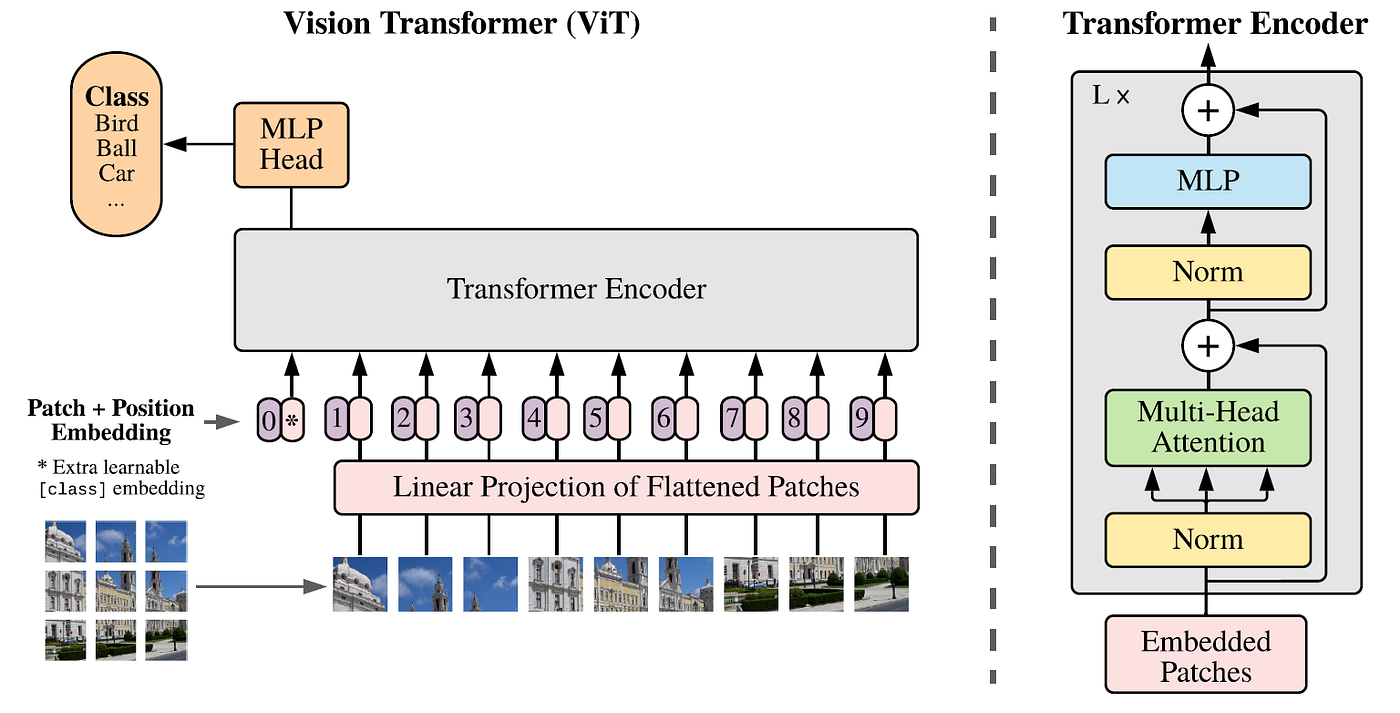
\includegraphics[width=0.7\textwidth]{imagenes/marco/ViT.png}
	\caption{Vision Transformer (ViT) architecture overview. The model processes an image as a sequence of patches through a standard Transformer encoder. Image taken from \cite{AnImageIsWorth}.}
	\label{fig:ViTArchitecture}
\end{figure}

\subsubsection{Object Classification and Representative Power}
The original ViT was designed and evaluated primarily on Object Classification, the task introduced in Section~\ref{sec:framework:cv} that also serves as the setting for the Continual Learning problem studied in this thesis. By attending over the full sequence of patch tokens rather than a local receptive field, ViTs have shown they can match or exceed CNN performance on this task, particularly when pre-trained on the kind of large-scale datasets described below.

\subsubsection{Self-Supervised Advancements: DINOv2}

Most vision datasets are still built around labels assigned by hand, but recent work has shifted toward foundation models trained via self-supervised learning instead, following the same general pre-training paradigm described earlier in this chapter: no human-provided labels are used at all. A leading example of this approach is \textbf{DINOv2} \cite{oquab2024dinov}, which produces visual features that are robust and general enough to perform well ``out of the box,'' both at the level of whole-image descriptions and at the level of individual patch tokens.

DINOv2 is built around a \textbf{Student-Teacher self-distillation} framework, extending earlier work on DINO \cite{DINO} and iBOT \cite{ibot}. Two networks of identical architecture are trained in parallel: a \textit{Student} network $g_{\theta_s}$, whose weights are updated by gradient descent as usual, and a \textit{Teacher} network $g_{\theta_t}$, which is never trained directly and instead tracks the student as an Exponential Moving Average (EMA) of its weights $\theta_s$:

\begin{equation}
	\theta_t \leftarrow \lambda \theta_t + (1 - \lambda) \theta_s
\end{equation}

where $\lambda \in [0, 1]$ is a smoothing parameter controlling how slowly the teacher follows the student. During training, the framework optimizes two complementary objectives to learn both global and fine-grained spatial representations:

\begin{itemize}
	\item \textbf{Image-Level Loss (DINO):} The student is fed both global and local crops of the same image, while the teacher only ever processes global views. The student is trained to match the teacher's output distribution over a set of learned prototype vectors, an online \textit{Sinkhorn-Knopp centering} step keeping this matching balanced so that the representations do not collapse to a single trivial solution.
	\item \textbf{Patch-Level Loss (iBOT):} To force the model to capture dense, local structure rather than only a global summary, a subset of the student's input patch tokens are masked out. The student must then reconstruct the teacher's corresponding patch-level features, computed from the same image without any masking.
	\item \textbf{KoLeo Regularization:} To keep the resulting embeddings spread out across the feature space rather than collapsing into a narrow region, DINOv2 adds a term based on the Kozachenko-Leonenko (KoLeo) differential entropy estimator, which penalizes feature vectors for lying too close to their nearest neighbor within a training batch:
	\begin{equation}
		\mathcal{L}_{\text{KoLeo}} = -\frac{1}{n}\sum_{i=1}^{n} \log \left( \min_{j \neq i} \| \vec{x}_i - \vec{x}_j \|_2 \right)
	\end{equation}
	where $\vec{x}_i$ is the $\ell_2$-normalized feature vector of the $i$-th image in a batch of size $n$.
\end{itemize}

\chapter{Statistical and Probabilistic Foundations of the Feature Space}
\label{ch:gaussian_space}

The framework proposed in this thesis rests on a single working hypothesis: that the class-conditional feature distributions produced by a frozen visual foundation model are well approximated by multivariate Gaussians, and that the resulting decision surfaces can be described in terms of the geometry of the embedding space they live in. This chapter puts together, in one self-contained treatment, the mathematical and statistical tools used throughout this thesis to build and check that hypothesis. We start with the probabilistic modelling framework itself---Bayesian inference, the Maximum A Posteriori decision rule, and its Mixture-of-Gaussians extension. We then turn directly to the Gaussianity assumption these models depend on, presenting the moment-based diagnostics and the formal hypothesis tests, univariate first and then multivariate, including the Henze--Zirkler statistic and its diagonal adaptation, that are later applied empirically in Chapter~\ref{ch:results}. With that assumption in place, we introduce the inter-class separability metrics---the probabilistic Bhattacharyya distance and the geometric Euclidean distance---used to quantify how classes crowd the embedding space as new tasks arrive. We then explain why estimating a covariance matrix in this setting is difficult in the first place, a difficulty commonly known as the curse of dimensionality, and how it can be addressed through regularization; this naturally leads into the spectral tools---Principal Component Analysis and the associated eigenvalue-decay diagnostics---used to describe the intrinsic dimensionality of the feature space and, in turn, to understand why that regularization is needed.

\section{Foundations of Probabilistic Modeling}
\label{sec:framework:probabilistic}

Representing each class as a Gaussian density only makes sense if there is a solid decision rule behind it that says how to actually use that density to classify a new observation. This section builds that rule from the ground up: starting from Bayes' theorem, we arrive at the Maximum A Posteriori (MAP) criterion, which tells us how to pick the most likely class given the observed features, and then extend it to mixtures of Gaussians for classes whose features are better described by more than one cluster. 
\subsection{Bayes Classification}

At its core, Bayes classification is rooted in \textbf{Bayes' Theorem}, which provides a mathematical framework for updating the probability of a hypothesis based on observed evidence. For a classification task, we seek the posterior probability $p(y=c \mid \vec{x})$—the probability that an observation belongs to class $c$ given its observed feature vector $\vec{x}$.

Bayes' Theorem is defined as:
\begin{equation}
	p(y=c \mid \vec{x}) = \frac{p(\vec{x} \mid y=c) \, p(y=c)}{p(\vec{x})}
\end{equation}
where:
\begin{itemize}
	\item $p(y=c \mid \vec{x})$ is the \textbf{posterior} probability.
	\item $p(\vec{x} \mid y=c)$ is the \textbf{likelihood} of the data given the class.
	\item $p(y=c)$ is the \textbf{prior} probability of the class.
	\item $p(\vec{x})$ is the \textbf{evidence} or marginal likelihood, acting as a normalization constant.
\end{itemize}

The objective of a Bayes classifier is to minimize the Bayes risk; in the simplest case, this corresponds to assigning the observation to the class that maximizes the posterior probability.

\subsection{Likelihood-Based Classification}

Likelihood inference provides a coherent framework for updating the probability of a hypothesis as more evidence or information becomes available. In contrast to frequentist approaches that treat parameters as fixed but unknown constants, the Bayesian paradigm treats parameters as random variables characterized by probability distributions.

The connection between Bayes' Theorem and likelihood-based classification lies in the \textbf{Maximum A Posteriori (MAP)} decision rule. Since the evidence $p(\vec{x})$ is constant across all classes for a given observation, the classification decision depends solely on the product of the likelihood and the prior:
\begin{equation}
	p(y=c \mid \vec{x}) \propto p(\vec{x} \mid y=c) \, p(y=c).
\end{equation}

A generative modeling framework can be adopted and class-conditional Gaussian feature distributions can be assumed:
\begin{equation}
	p(\vec{x} \mid y=c)
	=
	\mathcal{N}(\vec{x} \mid \boldsymbol{\mu}_c, \boldsymbol{\Sigma}_c),
\end{equation}
where $\vec{x} \in \mathbb{R}^d$ represents the feature vector, $\boldsymbol{\mu}_c$ is the class mean vector, and $\boldsymbol{\Sigma}_c \succ 0$ is the covariance matrix.

Classification can be performed via MAP inference by maximizing the log-posterior:
\begin{equation}
	\hat{y}
	=
	\arg\max_{c \in \mathcal{Y}}
	\left[
	\log p(\vec{x} \mid y=c) + \log \pi_c
	\right],
\end{equation}
where $\pi_c = p(y=c)$ denotes the class prior.

Substituting the multivariate Gaussian density into the MAP rule, the decision rule becomes equivalent to:
\begin{equation}
	\hat{y}
	=
	\arg\min_{c}
	\left[
	(\vec{x}-\boldsymbol{\mu}_c)^T
	\boldsymbol{\Sigma}_c^{-1}
	(\vec{x}-\boldsymbol{\mu}_c)
	+
	\log |\boldsymbol{\Sigma}_c|
	-
	2\log \pi_c
	\right].
\end{equation}

\subsubsection{Mixture of Gaussians (MoG)}

A Mixture of Gaussians models a complex probability density as a convex combination of $K$ distinct Gaussian components. This approach is fundamental for clustering and density estimation in multi-modal distributions. Therefore, to capture multimodal feature distributions, the class-conditional model can be extended to a mixture:

\begin{equation}
	p(\vec{x} \mid y=c)
	=
	\sum_{k=1}^{K_c}
	\alpha_{c,k}
	\mathcal{N}(\vec{x} \mid \boldsymbol{\mu}_{c,k}, \boldsymbol{\Sigma}_{c,k}),
\end{equation}
where $\alpha_{c,k} \ge 0$ and $\sum_k \alpha_{c,k} = 1$.

The MAP decision rule becomes
\begin{equation}
	\hat{y}
	=
	\arg\max_c
	\left[
	\log
	\left(
	\sum_{k=1}^{K_c}
	\alpha_{c,k}
	\mathcal{N}(\vec{x} \mid \boldsymbol{\mu}_{c,k}, \boldsymbol{\Sigma}_{c,k})
	\right)
	+
	\log \pi_c
	\right].
\end{equation}

This whole classification framework---from the plain Bayes rule to its Gaussian and mixture-of-Gaussians instantiations---is only as good as the assumption it is built on: that class-conditional features are actually well described by a Gaussian in the first place. The remainder of this chapter puts that assumption to work. Section~\ref{sec:method:gaussianity_main} tests it directly through moment-based diagnostics and formal hypothesis tests; Section~\ref{sec:method:separability} studies how the resulting Gaussians relate to one another as more classes are added; Section~\ref{sec:gsc:covariance} addresses the practical difficulty of estimating a covariance matrix $\boldsymbol{\Sigma}_c$ in a high-dimensional, small-sample regime; and Section~\ref{sec:gsc:spectral} closes the chapter by examining the geometric structure of the space these covariances live in.

\section{Gaussianity Assumptions and Analysis}
\label{sec:method:gaussianity_main}

The validity of the Bayes classifier introduced in Section~\ref{sec:framework:probabilistic} depends on how well the class-conditional Gaussian distributions approximate the true data distribution. The covariance estimators and downstream classification framework proposed in this thesis rest on the working assumption that class-conditional features are approximately Gaussian in the embedding space of visual foundation models (such as DINOv2). The following analytical framework establishes the statistical basis for these assumptions and, subsequently, the concrete methodology used to validate them empirically without relying on manual semantic labels, employing a multi-layered statistical evaluation on the training split of our datasets.

Our validation is structured across two levels, examined in that order in the rest of this section:
\begin{enumerate}
	\item \textbf{Per-Dimension (Univariate) Gaussianity:} Evaluated using moment-based shape diagnostics, the formal D'Agostino--Pearson omnibus normality test, and a coordinate-wise application of the Henze--Zirkler (HZ) test.
	\item \textbf{Per-Class (Multivariate) Gaussianity:} Evaluated in the native high-dimensional feature space using a specialized diagonal-covariance adaptation of the HZ test to circumvent sample-size rank deficiencies.
\end{enumerate}

\subsection{Univariate Gaussianity: Conceptual Diagnostics}
\label{sec:method:gaussianity:univariate_concept}

A first layer of theoretical justification involves examining the univariate properties of individual feature components: the kurtosis and skewness of each coordinate's marginal distribution.

\paragraph{Kurtosis} This statistic measures the ``tailedness'' and peakedness of a probability distribution relative to a normal distribution \cite{joyce2011kurtosis}. As illustrated in Figure \ref{fig:kurtosis}, a perfectly Gaussian distribution has an excess kurtosis of zero (mesokurtic). Distributions with high kurtosis (leptokurtic, $Kurtosis > 0$) exhibit sharper peaks and heavier tails, indicating a higher concentration of data around the mean and a greater likelihood of extreme outliers. Conversely, low kurtosis (platykurtic, $Kurtosis < 0$) indicates a flatter peak and thinner tails.

\begin{figure}[ht]
	\centering
	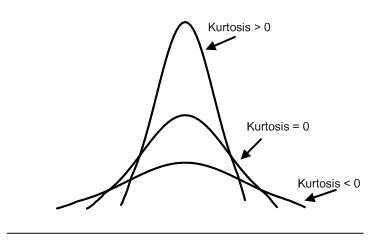
\includegraphics[width=0.37\textwidth]{imagenes/marco/kurtosis.png}
	\caption{Visual representation of kurtosis levels: leptokurtic ($>0$), mesokurtic ($=0$) and platykurtic ($<0$) distributions \cite{joyce2011kurtosis}.}
	\label{fig:kurtosis}
\end{figure}

\paragraph{Skewness} This measure quantifies the asymmetry of a distribution around its mean. As shown in Figure \ref{fig:skewness}, a symmetric distribution (center) is a fundamental assumption of the Gaussian model, implying that the mean $\boldsymbol{\mu}_c$, median, and mode coincide, providing an adequate representation of the class prototype within the embedding space. A positive skew (right) indicates a distribution with a long tail extending toward higher values, while a negative skew (left) indicates a long tail extending toward lower values. Significant skewness would suggest that the class-conditional mean is no longer a central representation of the feature distribution.

\begin{figure}[ht]
	\centering
	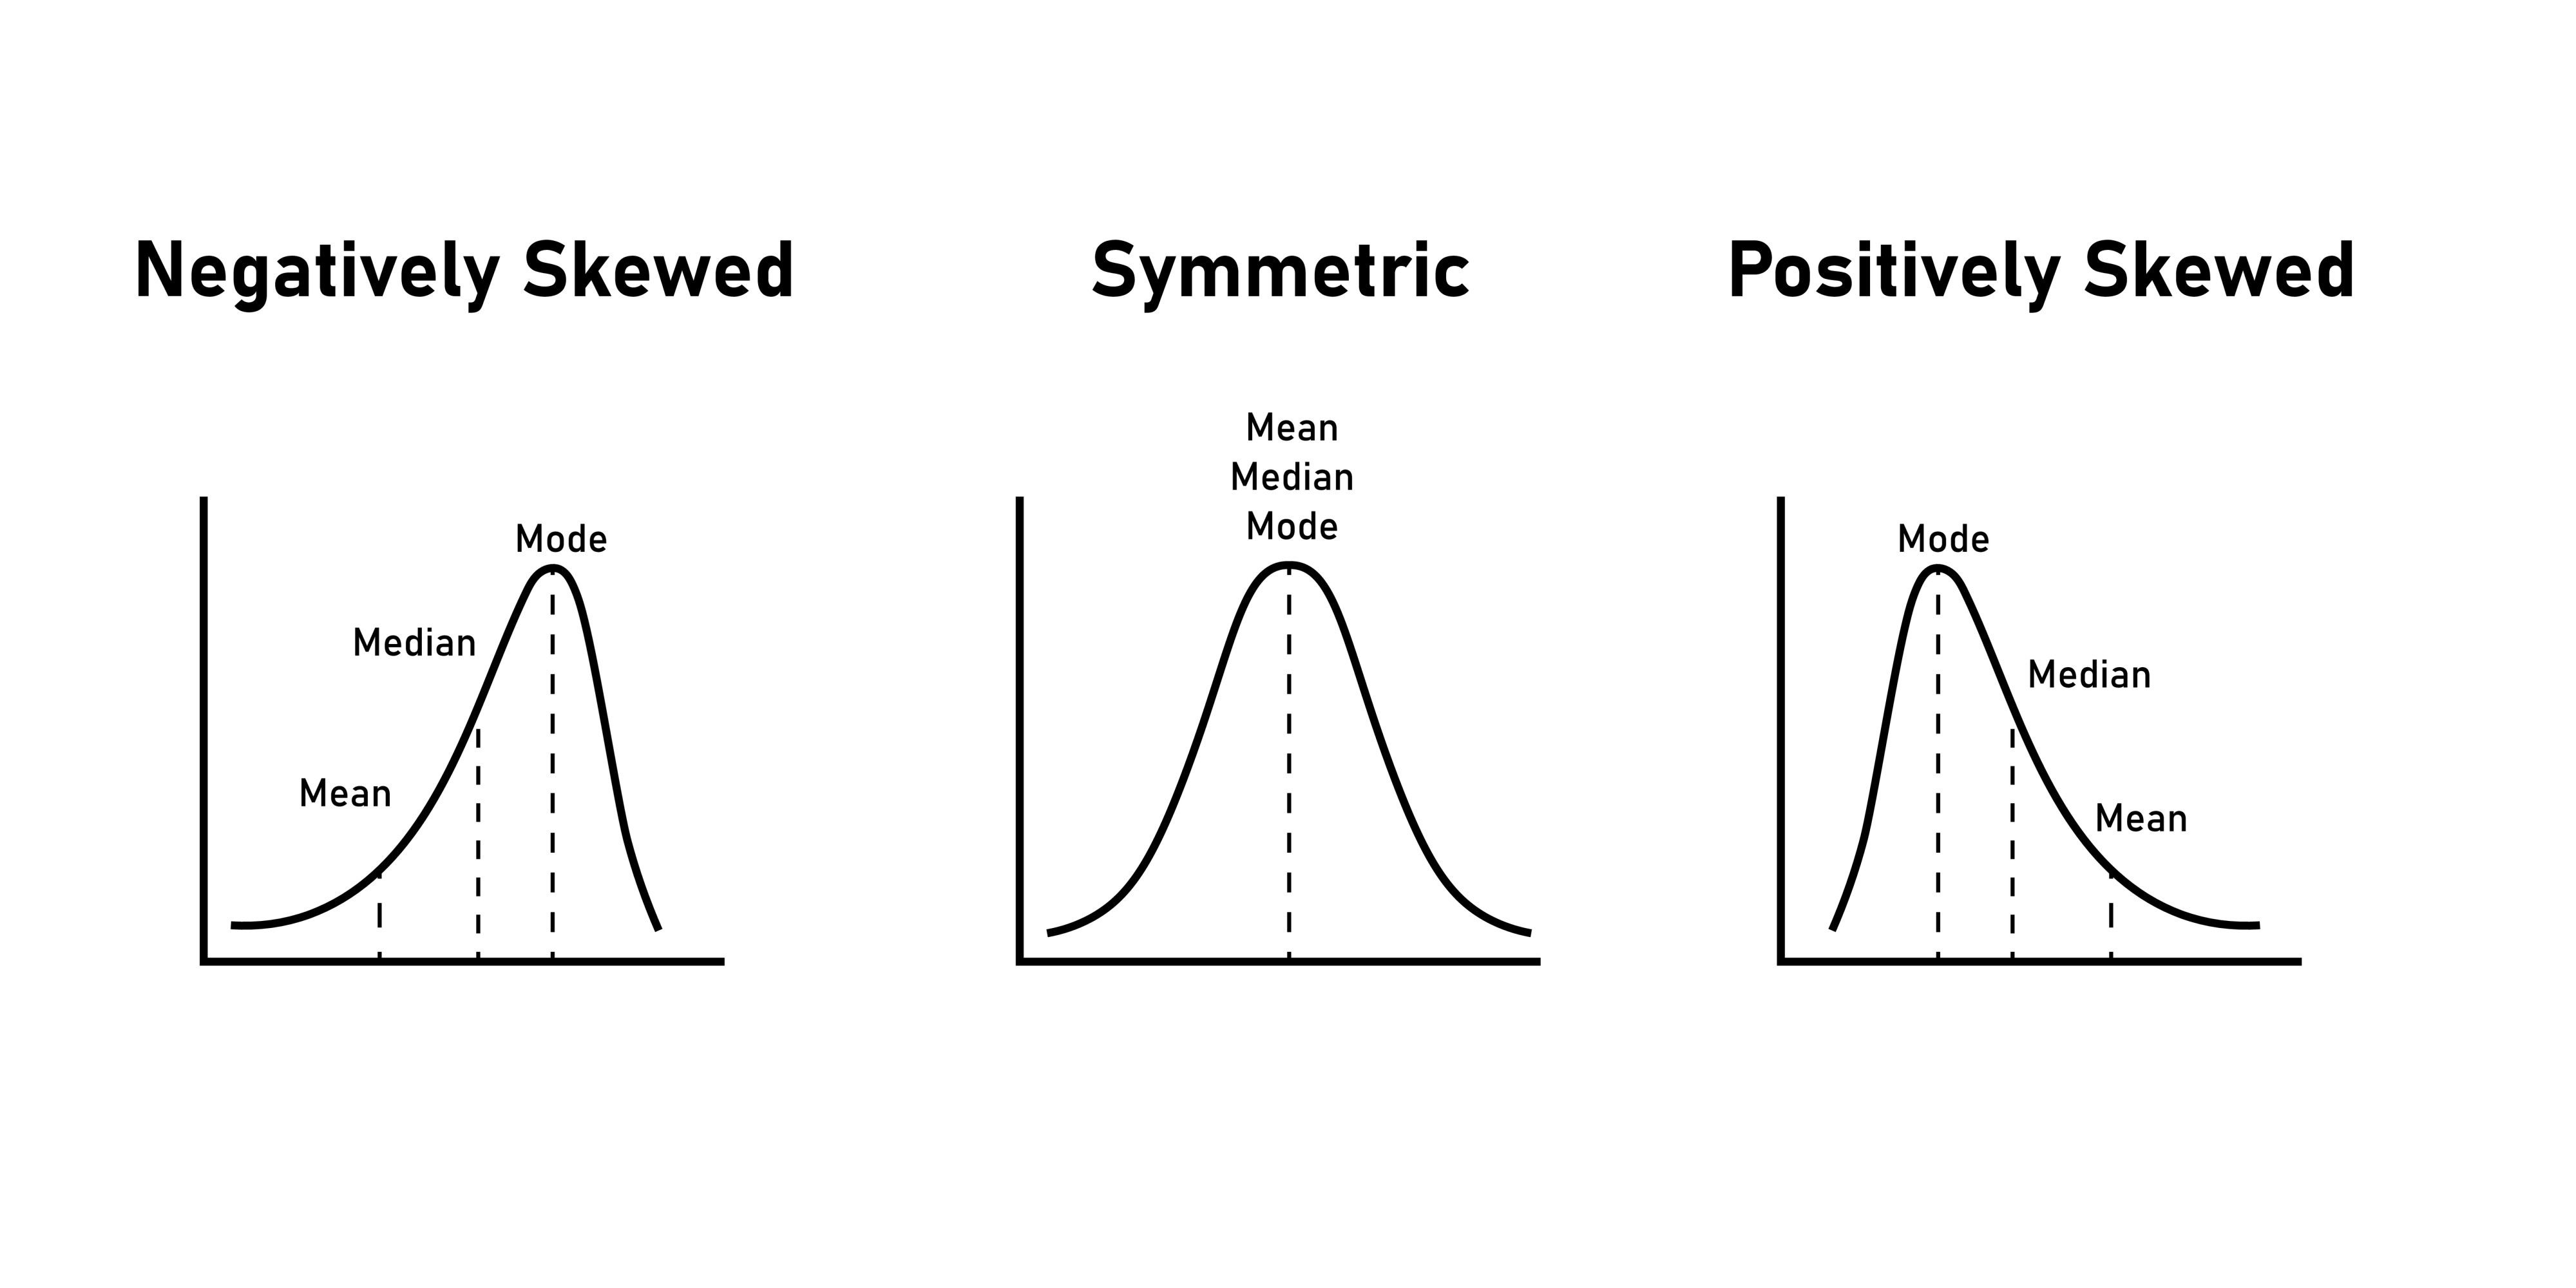
\includegraphics[width=0.7\textwidth]{imagenes/marco/skeweness.jpg}
	\caption{Comparison of negatively-skewed, symmetric and positively-skewed distributions \cite{pearson1895skewness}.}
	\label{fig:skewness}
\end{figure}

Taken together, these two diagnostics give an initial, coordinate-level read on how well the Gaussian approximation actually holds. Empirical evidence suggests that for many real-world datasets, both kurtosis and skewness values typically fall within the range $[-1,1]$ tails \cite{hair2019multivariate}, indicating distributions that are close to symmetric and free of excessively heavy.

\subsection{Per-Dimension Gaussianity: Moments and Formal Tests}
\label{sec:method:gaussianity:moments}
\phantomsection\label{sec:method:gaussianity:normaltest}

Building on the conceptual diagnostics above, we now formalize the per-dimension analysis into a concrete testing methodology. To verify Gaussianity at the level of individual feature coordinates, we apply three complementary indicators to every (class~$c$, dimension~$j$) pair.

\subsubsection{Shape moments.}
Following the normality diagnostics of Pearson~\cite{pearson1895skewness} and D'Agostino and Pearson~\cite{dagostino1971omnibus,dagostino1973tests}, we compute the sample skewness and excess kurtosis for each class~$c$ along each of the $d$ coordinates:
\begin{equation}
	\widehat{\mathrm{Skew}}_{c,j} \;=\; \frac{\frac{1}{n_c}\sum_{i}(x_{i,j}-\mu_{c,j})^3}{\hat\sigma_{c,j}^{3}},\qquad
	\widehat{\mathrm{Kurt}}_{c,j} \;=\; \frac{\frac{1}{n_c}\sum_{i}(x_{i,j}-\mu_{c,j})^4}{\hat\sigma_{c,j}^{4}} - 3,
	\label{eq:moments}
\end{equation}
where both quantities vanish exactly for a theoretical Gaussian distribution~\cite{pearson1895skewness,joyce2011kurtosis}.

\subsubsection{D'Agostino--Pearson omnibus test.}
The moments alone do not constitute a formal statistical test. We therefore apply the D'Agostino--Pearson omnibus test to every (class, dimension) pair~\cite{dagostino1971omnibus,dagostino1973tests}. The test combines the two shape statistics into a single composite statistic:
\begin{equation}
	K^2 \;=\; Z_1\!\left(\widehat{\mathrm{Skew}}\right)^2 + Z_2\!\left(\widehat{\mathrm{Kurt}}\right)^2 \;\sim\; \chi^2_2 \quad \text{under } H_0,
	\label{eq:normaltest}
\end{equation}
where $Z_1$ and $Z_2$ are normalised transformations of the skewness and kurtosis estimators respectively, and $H_0$ is the hypothesis that the marginal data are normally distributed. We reject $H_0$ at significance level $\alpha=0.05$.

\subsubsection{Relaxed criterion.}
Because the omnibus test is highly sensitive to larger sample sizes $n_c$ (where minor, non-critical departures from perfect normality still accumulate into significant $K^2$ values), we supplement it with a size-independent relaxed indicator. A dimension is classified as near-Gaussian if:
\begin{equation}
	|\mathrm{Skew}| < 1 \quad \text{and} \quad |\mathrm{Kurt}| < 1
\end{equation}
hold simultaneously. This relaxed criterion acts alongside the strict omnibus test to establish lower and upper bounds on the proportion of approximately Gaussian coordinates.

\subsection{The Henze--Zirkler Test}
\label{sec:method:gaussianity:hz_theory}

The diagnostics above operate one coordinate at a time, so they cannot pick up on dependencies between coordinates: a set of features can each look perfectly normal on their own while their joint distribution still departs from a proper multivariate Gaussian. The Henze--Zirkler (HZ) test~\cite{henze1990class} closes this gap: it is an omnibus test, applicable to a feature vector of any dimension $d$, that compares the empirical characteristic function of the data against the theoretical characteristic function of a multivariate normal distribution.

Given $n$ centred samples $\vec{z}_i = \vec{x}_i - \hat{\boldsymbol{\mu}}_c$ and a smoothing bandwidth $b > 0$, the test statistic is built from three terms evaluated using the squared Mahalanobis distances $d_M^2(\cdot,\cdot)$ induced by the class covariance $\boldsymbol{\Sigma}_c$:

\begin{equation}
	A = \frac{1}{n^2} \sum_{j=1}^{n} \sum_{k=1}^{n} e^{-\frac{b^2}{2}d_M^2(\vec{z}_j, \vec{z}_k)},
\end{equation}
\begin{equation}
	B = \frac{2}{n}(1+b^2)^{-d/2} \sum_{j=1}^{n} e^{-\frac{b^2}{2(1+b^2)}d_M^2(\vec{z}_j, \vec{0})},
\end{equation}
\begin{equation}
	C = (1+2b^2)^{-d/2}.
\end{equation}

Term $A$ measures the average pairwise kernel similarity of the observed samples; term $B$ quantifies how consistently the empirical density decays away from the class centroid compared to a Gaussian; and term $C$ is the asymptotic self-similarity constant of a true $d$-dimensional Gaussian. The final statistic is:
\begin{equation}
	T_{n,b} = n \cdot \left[ A - B + C \right].
\end{equation}

Under the null hypothesis of multivariate normality, $T_{n,b}$ converges to a fixed value close to $1$; departures above $1$ indicate that the data is more structured (tighter clusters or heavier tails) than a Gaussian. The bandwidth $b$ controls the resolution of the characteristic function comparison and is set optimally as a function of $n$ and $d$. The next two subsections apply this same statistic to two settings that differ only in dimensionality: first the univariate case ($d=1$), applied per coordinate as a stricter complement to the tests above, and then the full, high-dimensional multivariate case ($d=768$) that the classifier actually operates in.

\subsection{Univariate Henze-Zirkler Test per Dimension}
\label{sec:method:gaussianity:hz_univariate}

We bridge the per-dimension and per-class analyses by introducing a univariate HZ analysis applied independently to every (class~$c$, dimension~$j$) pair. This provides a stricter hypothesis-based criterion than the D'Agostino--Pearson test, while remaining more interpretable than the full-dimensional multivariate result presented next.

\paragraph{Bandwidth.}
For $d=1$, the standard HZ smoothing parameter reduces to:
\begin{equation}
	b^2 \;=\; \frac{1}{2}\left(\frac{4}{3}\right)^{2/5} n_c^{-2/5}.
	\label{eq:hz_bw_univariate}
\end{equation}

\paragraph{Efficient vectorised computation.}
To handle all $d$ dimensions simultaneously without forming prohibitive $n_c \times n_c$ distance matrices, the pairwise kernel term in $T_{\mathrm{HZ}}$ is expanded via its Taylor series around $b^2 x_j x_k = 0$:
\begin{equation}
	A_m \;=\; \frac{1}{n_c^2}\sum_{j,k} e^{-\frac{b^2}{2}(z_{j,m}-z_{k,m})^2}
	\;=\; \frac{1}{n_c^2}\sum_{\ell=0}^{L}
	\frac{b^{2\ell}}{\ell!}\,S_\ell^2\;+\;\mathcal{O}\!\left((b^2)^{L+1}\right),
	\label{eq:hz_taylor}
\end{equation}
where $S_\ell = \sum_j v_{j,m}\,z_{j,m}^\ell$, $v_{j,m} = \exp(-b^2 z_{j,m}^2 / 2)$, and $L=8$ terms are used to keep the approximation error below $10^{-6}$.

\paragraph{Expected value under $H_0$ and p-value.}
For a general $d$-dimensional problem, the asymptotic expected value of $T_{\mathrm{HZ}}$ under exact normality is:
\begin{equation}
	\mathbb{E}_{H_0}[T_{\mathrm{HZ}}] \;=\; 1 - (1 + 2b^2)^{-d/2},
	\label{eq:hz_expected_general}
\end{equation}
which is the reference used for the multivariate diagonal test of Section~\ref{sec:method:gaussianity:multivariate} ($d=768$): even a modest bandwidth causes $(1+2b^2)^{-d/2}\to 0$ for large $d$, driving $\mathbb{E}_{H_0}[T_{\mathrm{HZ}}]\to 1$.

For the univariate case ($d=1$) treated in this section, we instead use the exact finite-sample expectation, which includes higher-order correction terms that the large-$d$ asymptotic approximation of Equation~\eqref{eq:hz_expected_general} discards:
\begin{equation}
	\mathbb{E}_{H_0}[T_{\mathrm{HZ}}] \;=\; 1 - a^{-1/2}\left(1 + \frac{b^2}{a} + \frac{3b^4}{4a^2}\right), \qquad a = 1+2b^2,
	\label{eq:hz_expected_univariate}
\end{equation}
with $b^2$ given by the bandwidth of Equation~\eqref{eq:hz_bw_univariate}.

Under the null hypothesis $H_0$ of perfect univariate normality, we theoretically expect the empirical statistic $T_{\mathrm{HZ}}$ to be close to $0$. For the class sizes encountered here ($n_c \in [60,\,400]$), the adaptive bandwidth is small ($b^2 \approx 0.04$), which yields a baseline expectation of $\mathbb{E}_{H_0}[T_{\mathrm{HZ}}] \approx 0.04$. Consequently, any coordinate that is genuinely Gaussian will yield an empirical $T_{\mathrm{HZ}}$ value fluctuating tightly around this near-zero baseline, in contrast to the high-dimensional multivariate case where $T_{\mathrm{HZ}} \to 1$.

\subsection{Per-Class Gaussianity: Diagonal Henze--Zirkler Adaptation}
\label{sec:method:gaussianity:multivariate}

Having applied the HZ statistic one coordinate at a time, we now turn to its genuinely multivariate use: testing the joint, $d$-dimensional distribution of each class directly. Computing a standard full-covariance HZ test is mathematically intractable in high-dimensional spaces where the per-class sample size is smaller than the feature dimensionality ($n_c < d$). Under these conditions, the empirical covariance matrix becomes singular and non-invertible, preventing the calculation of standard Mahalanobis distances.

To circumvent this rank deficiency without resorting to destructive dimensionality reduction, we formulate a diagonal-covariance adaptation of the HZ test. The required Mahalanobis distances are computed analytically by inverting only the $d$ per-coordinate sample variances (effectively regularizing the space), with a numerical floor of $\varepsilon=10^{-10}$ applied to guard against inactive dimensions:
\begin{equation}
	\mathbb{E}[T_{\mathrm{HZ}}] \;=\; 1 - (1+2b^2)^{-d/2} \;\to\; 1 \quad \text{as } d \to \infty,
	\label{eq:hz_expected}
\end{equation}
meaning that values concentrated near $T_{\mathrm{HZ}} \approx 1$ serve as the Gaussian reference under the diagonal model.

Having established, at both the univariate and multivariate levels, how well class-conditional features actually satisfy the Gaussianity assumption, we now turn to how these Gaussians are positioned \emph{relative to one another} within the embedding space.

\section{Inter-Class Structural Separability Analysis}
\label{sec:method:separability}

To understand how the Bayesian decision surface scales and characterize the geometric crowding of the embedding space as new tasks are incorporated, we evaluate inter-class relationships using two complementary metrics: the probabilistic Bhattacharyya distance and the geometric Euclidean distance.

\subsection{Pairwise Bhattacharyya Distance}
\label{sec:method:separability:bhattacharyya}

The \emph{inter-class} pairwise Bhattacharyya distance measures how distinguishable any two class-conditional Gaussians are from one another.
The Bhattacharyya distance is symmetric and provides a direct connection to the Bayes error rate via the Bhattacharyya coefficient $\rho_{ij} = e^{-D_B(i,j)}$.
Under the diagonal-Gaussian parameterisation, the Bhattacharyya distance between classes $i$ and $j$ is defined as:
\begin{equation}
	D_B(i,j)
	= \frac{1}{8}(\boldsymbol{\mu}_i - \boldsymbol{\mu}_j)^{\top}
	\bar{\Sigma}^{-1}
	(\boldsymbol{\mu}_i - \boldsymbol{\mu}_j)
	+ \frac{1}{2}\ln\!\left(
	\frac{\det\bar{\Sigma}}{\sqrt{\det\Sigma_i\,\det\Sigma_j}}
	\right),
	\label{eq:interclass_bhattacharyya}
\end{equation}
where $\bar{\Sigma} = (\Sigma_i + \Sigma_j)/2$.
Because both $\Sigma_i$ and $\bar{\Sigma}$ are diagonal, all matrix operations reduce to element-wise arithmetic: determinants become products of the diagonal entries (or sums of logs), and the matrix inverse reduces to element-wise reciprocals.
A value of $D_B=0$ indicates complete distributional overlap; larger values correspond to greater separability and a lower Bhattacharyya coefficient $\rho = e^{-D_B}$.

\subsection{Pairwise Mean Euclidean Distance}
\label{sec:method:separability:euclidean}

While the Bhattacharyya distance jointly accounts for shifts in both first-order (means) and second-order (covariances) statistics, it can mask whether class texturing or raw prototype drift is the dominant factor in class confusion. Therefore, we isolate first-order geometric separation by calculating the plain pairwise Euclidean distance between the estimated class mean vectors $\boldsymbol{\mu}_i$ and $\boldsymbol{\mu}_j$:
\begin{equation}
	d_E(i,j) = \|\boldsymbol{\mu}_i - \boldsymbol{\mu}_j\|_2 = \sqrt{\sum_{k=1}^{d} (\mu_{i,k} - \mu_{j,k})^2},
	\label{eq:interclass_euclidean}
\end{equation}
where $d$ is the nominal dimensionality of the visual foundation embedding space.

\subsection{Stream Statistics and Trajectory Tracking}
\label{sec:method:separability:tracking}

As the total number of observed classes $k$ scales throughout the continual learning stream, we track three distinct statistics for both $D_B$ and $d_E$ across the expanding class-pair pool:
\begin{enumerate}
	\item[(a)] The \textbf{macro-averaged pairwise distance} ($\overline{D_B}$ and $\overline{d_E}$) flanked by a $[\mathrm{P}_{10},\mathrm{P}_{90}]$ percentile band to observe global drift.
	\item[(b)] The \textbf{minimum pairwise distance} ($\min D_B$ and $\min d_E$), which explicitly identifies the hardest, most confusable class pair in the system.
	\item[(c)] The \textbf{cumulative count of overlapping pairs} falling below critical proximity thresholds (e.g., $D_B \in \{10, 50, 100\}$ and $d_E \in \{0.3, 0.5, 0.7\}$) to capture the heavy-tailed growth of localized confusion sinks.
\end{enumerate}
Together, these metrics bridge empirical classification failure modes with the underlying statistical architecture of the learned representations.

The separability picture above already hints at why estimating each class's covariance matrix reliably matters so much: as classes crowd closer together, small errors in $\Sigma_c$ translate directly into decision-surface errors. We now look at why that estimation is difficult in the first place, and how it can be made reliable in the high-dimensional, small-sample regime this thesis operates in.

\section{Covariance Estimation in High-Dimensional Spaces}
\label{sec:gsc:covariance}

A fundamental challenge in multivariate statistical analysis and pattern recognition is the estimation of the covariance matrix $\boldsymbol{\Sigma} \in \mathbb{R}^{d \times d}$ from a finite set of $n$ observations. In classical low-dimensional regimes, where the sample size $n$ is much larger than the feature dimension $d$ ($n \gg d$), the empirical Sample Covariance Matrix (SCM) acts as a reliable, unbiased estimator. However, modern engineering applications—such as analyzing high-dimensional deep feature representations—frequently operate in the ``high-dimension, small-sample-size'' (HDSS) regime, where $d$ is of the order of hundreds or thousands, while $n$ remains strictly limited.

Under these conditions, classical multivariate analysis suffers severely from the \textit{curse of dimensionality}, leading to critical theoretical and numerical breakdowns in statistical modeling.

\subsection{The Curse of Dimensionality and Covariance Degeneracy}

When the dimensionality $d$ scales while the sample size $n$ remains fixed or grows at a slower rate, several geometric and algebraic anomalies emerge:

\begin{itemize}
	\item \textbf{Singularity and Rank Deficiency:} Structurally, the SCM is calculated as the sum of $n$ outer products of centered data vectors. Consequently, the maximum rank of the SCM is bounded by $\min(n-1, d)$. In the typical HDSS scenario where $n < d$, the SCM has at least $d - n + 1$ zero eigenvalues. The resulting matrix is singular (rank-deficient) and cannot be inverted.

	\item \textbf{Loss of Negative Log-Likelihood and Distance Metrics:} Many fundamental statistical classifiers and density estimators—such as Gaussian Discriminant Analysis (GDA) or Mahalanobis distance formulations—depend heavily on the precision matrix (the inverse covariance, $\boldsymbol{\Sigma}^{-1}$) and the log-determinant $\ln|\boldsymbol{\Sigma}|$. When the estimated covariance is singular, the log-determinant diverges to $-\infty$, and the precision matrix is undefined, rendering density estimation mathematically impossible.

	\item \textbf{Eigenvalue Distortion (Spreading Phenomenon):} Even in moderately high dimensions where $n \ge d$ and the SCM is technically invertible, the sample eigenvalues do not converge to their true counterparts. As proved in random matrix theory (e.g., the Marčenko-Pastur law \cite{MarPas67}), high-dimensional sample eigenvalues exhibit severe bias: the largest eigenvalues are systematically overestimated, while the smallest eigenvalues are underestimated. This artificial dispersion distorts the perceived geometric structure of the data.
\end{itemize}

\subsection{Theoretical Foundations of Regularization}

To overcome the numerical and structural instability of the empirical SCM in high dimensions, the theoretical framework must transition from pure maximum likelihood estimation toward \textit{regularization}. The conceptual objective is to trade a manageable amount of bias for a drastic reduction in estimator variance.

Conceptually, these regularized estimation strategies fall into two primary paradigms:

\begin{enumerate}
	\item \textbf{Spectral Regularization and Conditioning:} These approaches directly manipulate the empirical eigenspectrum. By placing a lower bound on near-zero eigenvalues or adding a perturbation matrix (e.g., diagonal loading), they artificially bound the condition number of the matrix. This guarantees strict positive definiteness ($\boldsymbol{\Sigma} \succ 0$), ensuring that the precision matrix remains numerically stable during inversion.

	\item \textbf{Structured Shrinkage:} Shrinkage theory, pioneered by Stein's loss formulations, constructs an estimator as a convex combination of the high-variance SCM and a low-variance structured ``target'' matrix (such as the identity matrix or a diagonal variance matrix). By shrinking the empirical estimator toward a well-behaved target, these methods systematically pull the distorted, spread-out eigenvalues back toward their true mean, minimizing the expected mean squared error.
\end{enumerate}

These two regularisation paradigms motivate the family of covariance estimators used throughout this thesis---diagonal, full, hybrid, shared, OAS, and Ledoit--Wolf---each trading a different amount of bias for a reduction in estimator variance. The eigenvalue anomalies described above are, at their root, a question of how variance is distributed across the $d$ coordinates of the feature space; we now turn to the spectral tools used to expose that distribution directly.

\section{Spectral Geometry and Dimensionality of the Feature Space}
\label{sec:gsc:spectral}

The validity of high-dimensional Gaussian modelling, and the practical behaviour of the covariance estimators just introduced, are both governed by the spectral structure of the embedding space: the way in which variance is distributed across the $d$ coordinates of the feature vector $\vec{x} \in \mathbb{R}^d$. We first develop Principal Component Analysis (PCA) as the analytical tool used to expose this structure, and then use it to define the effective dimensionality of the feature space and to design a controlled dimension-reduction probe.

\subsection{Principal Component Analysis}
\label{sec:marco:pca}

Principal Component Analysis (PCA) is a linear dimensionality-reduction technique that finds an orthonormal basis for the data by diagonalising the empirical covariance matrix~\cite{jolliffe2002principal}. Given a centred data matrix $\mathbf{X} \in \mathbb{R}^{N \times d}$ (zero-mean columns), the empirical covariance is

\begin{equation}
\mathbf{S} = \frac{1}{N-1}\mathbf{X}^{T}\mathbf{X}.
\end{equation}

Its eigendecomposition $\mathbf{S} = \mathbf{P}\boldsymbol{\Lambda}\mathbf{P}^{T}$ yields orthonormal eigenvectors $\mathbf{P} = [\mathbf{p}_1, \ldots, \mathbf{p}_d]$ sorted so that the corresponding eigenvalues satisfy $\lambda_1 \ge \lambda_2 \ge \cdots \ge \lambda_d \ge 0$. Each eigenvector $\mathbf{p}_i$ is a \emph{principal component} (PC), and $\lambda_i$ equals the variance of the data projected onto $\mathbf{p}_i$.

\paragraph{Dimensionality reduction.}
Retaining only the leading $k$ eigenvectors defines the projection matrix $\mathbf{P}_k = [\mathbf{p}_1, \ldots, \mathbf{p}_k] \in \mathbb{R}^{d \times k}$. A new observation $\vec{x} \in \mathbb{R}^d$ is mapped to a $k$-dimensional representation via

\begin{equation}
\tilde{\vec{x}} = \mathbf{P}_k^{T}(\vec{x} - \boldsymbol{\mu}),
\label{eq:pca_project}
\end{equation}

where $\boldsymbol{\mu}$ is the global mean estimated from the training corpus. The resulting coordinates $\tilde{\vec{x}}$ are decorrelated: $\operatorname{Cov}(\tilde{\vec{x}}) = \operatorname{diag}(\lambda_1, \ldots, \lambda_k)$. The fraction of total variance preserved by the projection is

\begin{equation}
R(k) = \frac{\sum_{i=1}^{k}\lambda_i}{\sum_{i=1}^{d}\lambda_i}.
\end{equation}

\paragraph{Optimality and geometric interpretation.}
Among all rank-$k$ linear projections, PCA minimises the mean-squared reconstruction error and maximises the variance of the projected data (Eckart--Young theorem~\cite{eckart1936approximation}). Geometrically, the projected subspace aligns with the axes of the data ellipsoid along which the observations spread most.

\paragraph{Application to high-dimensional embeddings.}
When the original dimension $d$ is large (e.g.\ $d=768$ for DINOv2 ViT-B/14) but the data occupy a low-dimensional subspace---as evidenced by rapid eigenvalue decay---reducing to $k \ll d$ dimensions before downstream classification offers two complementary benefits: (i) it concentrates the discriminative signal in fewer coordinates, potentially improving the accuracy of subsequent covariance estimators; and (ii) it reduces computational cost by a factor of $\mathcal{O}((d/k)^2)$ for quadratic (Mahalanobis) classifiers. The trade-off is that components beyond $k$ are discarded, which may remove residual discriminative information if the spectrum does not decay quickly enough.

\subsection{Spectral Decay and Effective Dimensionality}
\label{sec:gsc:spectral_decay}

The practical validity of high-dimensional Gaussian modeling is further supported by examining the spectral structure of the feature space through Principal Component Analysis. The covariance of the class-mean-centred embeddings can be decomposed as $\boldsymbol{\Sigma} = \mathbf{P}\boldsymbol{\Lambda}\mathbf{P}^T$, where the diagonal of $\boldsymbol{\Lambda}$ contains the eigenvalues $\lambda_1 \ge \lambda_2 \ge \dots \ge \lambda_d \ge 0$ and $\mathbf{P}$ holds the corresponding orthonormal eigenvectors.

\paragraph{Variance concentration.}
If the eigenvalue spectrum decays steeply---most variance is explained by the first $k \ll d$ components---then the effective dimensionality of the feature distribution is much lower than the nominal $d$. Concretely, the fraction of variance explained by the leading $k$ components is $\sum_{i=1}^{k}\lambda_i \,/\, \sum_{i=1}^{d}\lambda_i$.

\subsection{Global Spectral Analysis of the Foundation Embeddings}
\label{sec:method:spectral:analysis}

To characterize the global variance distribution of the foundation feature space independently of individual class-conditional labels, we compute the empirical eigenspectrum of the $\ell_2$-normalised embeddings pooled across the entirety of each benchmark's training split. The $d=768$ eigenvalues ($\lambda_1 \ge \lambda_2 \ge \dots \ge \lambda_d \ge 0$) of the pooled data covariance matrix are sorted in descending order to analyze individual percentage-of-variance contributions and the cumulative explained variance.

This diagnostic explicitly measures the \emph{effective intrinsic dimensionality} of the shared representation. A rapid, steep eigenvalue decay implies that the visual discriminative signal is concentrated within a tight, low-dimensional active subspace, pointing to high structural redundancy in the ambient space. Conversely, a slow, uniform decay indicates an isotropic distribution where discriminative information is scattered widely across the full ambient space. Furthermore, this global spectral profile establishes a strict theoretical upper bound on the effective rank available to the localized, per-class covariance estimators, as a class-specific model can only populate directional parameters already spanned by the pooled population spectrum.

\subsection{Downstream PCA Dimension-Reduction Probing}
\label{sec:method:spectral:pca_test}

While the spectral analysis of Section~\ref{sec:method:spectral:analysis} describes the native distribution of the features, it does not evaluate whether a low-dimensional concentration can be systematically exploited to alleviate the high-dimensional small-sample rank deficiency ($n_c < d$) highlighted in Section~\ref{sec:gsc:covariance}. To establish a diagnostic boundary on performance under forced compression, we introduce a downstream PCA dimension-reduction test.

Rather than fitting a localized, data-dependent Principal Component Analysis on each target stream---which would violate the strict class-incremental constraints by altering the projection matrix over time---we utilize a fixed, out-of-distribution linear projection matrix $\mathbf{P}_k \in \mathbb{R}^{d \times k}$. This projection matrix is pre-trained exclusively on the supervised distribution of the \emph{ImageNet-21k} corpus, acting as a general-purpose, dataset-agnostic structural probe.

For a chosen reduced target dimensionality $k \in \{64, 256\}$, the $\ell_2$-normalized foundation features $\mathbf{x} \in \mathbb{R}^d$ are projected into a compressed subspace via:
\begin{equation}
	\tilde{\mathbf{x}} = \mathbf{P}_k^{\top} (\mathbf{x} - \boldsymbol{\mu}_{\text{global}}),
	\label{eq:pca_projection}
\end{equation}
where $\boldsymbol{\mu}_{\text{global}}$ is the stationary global mean of the pre-training corpus. The class-conditional Gaussian classifiers (both Diagonal and Full covariance parameterisations) are subsequently initialized, trained, and evaluated entirely within this frozen, low-dimensional coordinate system.

The relative scaling of accuracy and estimator stability across these reduced dimensions serves as a multi-faceted probe into the underlying geometry:

The robustness of downstream CIL performance under forced compression ($k \ll d$) demonstrates an alignment between the current discriminative signal and the leading principal axes of the supervised out-of-distribution probe, confirming that trailing variances act primarily as non-essential noise. Conversely, a pronounced accuracy degradation alongside decreasing dimensionality reveals that fine-grained inter-class decision boundaries remain heavily reliant on the long tail of the spectrum, rendering the full ambient high-dimensional space mandatory for preserving the class representations.

Furthermore, the relative performance gap between the Full and Diagonal covariance models exposes the interaction between subspace compression and data scarcity. A narrowing of the gap at lower dimensionalities indicates that the regularizing effect of the projection successfully mitigates the small-sample rank deficiency of the SCM. In contrast, a wider divergence or a systemic drop in Full covariance precision points to a structural distortion of underlying class-conditional correlations induced by the linear transformation.

Having established the geometry of the feature space---its Gaussianity, its inter-class separability, and its spectral structure---this chapter's characterization of the feature space is complete. Chapter~\ref{ch:results} applies these tools to the empirical results of the proposed framework, beginning with the average accuracy and forgetting scores that quantify raw continual-learning performance, and, immediately after them, the confidence and calibration metrics used to judge how reliable those predictions actually are.

\chapter{Modelling Class Densities in a Frozen Feature Space}
\label{methodology}

\section{Proposed Architecture}

As shown in Figure~\ref{fig:architecture}, our CIL framework is built upon a simple yet structurally motivated decomposition: (i) a frozen feature extractor based on a visual foundation model, and (ii) a probabilistic classification layer that models each object category through an independent Gaussian distribution in the embedding space. Given an input image, the feature extractor maps it to a fixed high-dimensional representation. For each class, we maintain a class-conditional multivariate Gaussian characterized by its mean vector and covariance matrix, estimated incrementally from observed samples. Classification is performed according to the maximum likelihood principle, assigning the input to the class whose Gaussian model yields the highest likelihood under the stationary embedding representation. This modular separation between representation learning and statistical modeling enables incremental updates without backpropagation or parameter adaptation: adding a new class requires only estimating its distribution in the fixed feature space, while previously learned classes remain unaffected at the representation level.

\begin{figure}[htb]
	\centering
	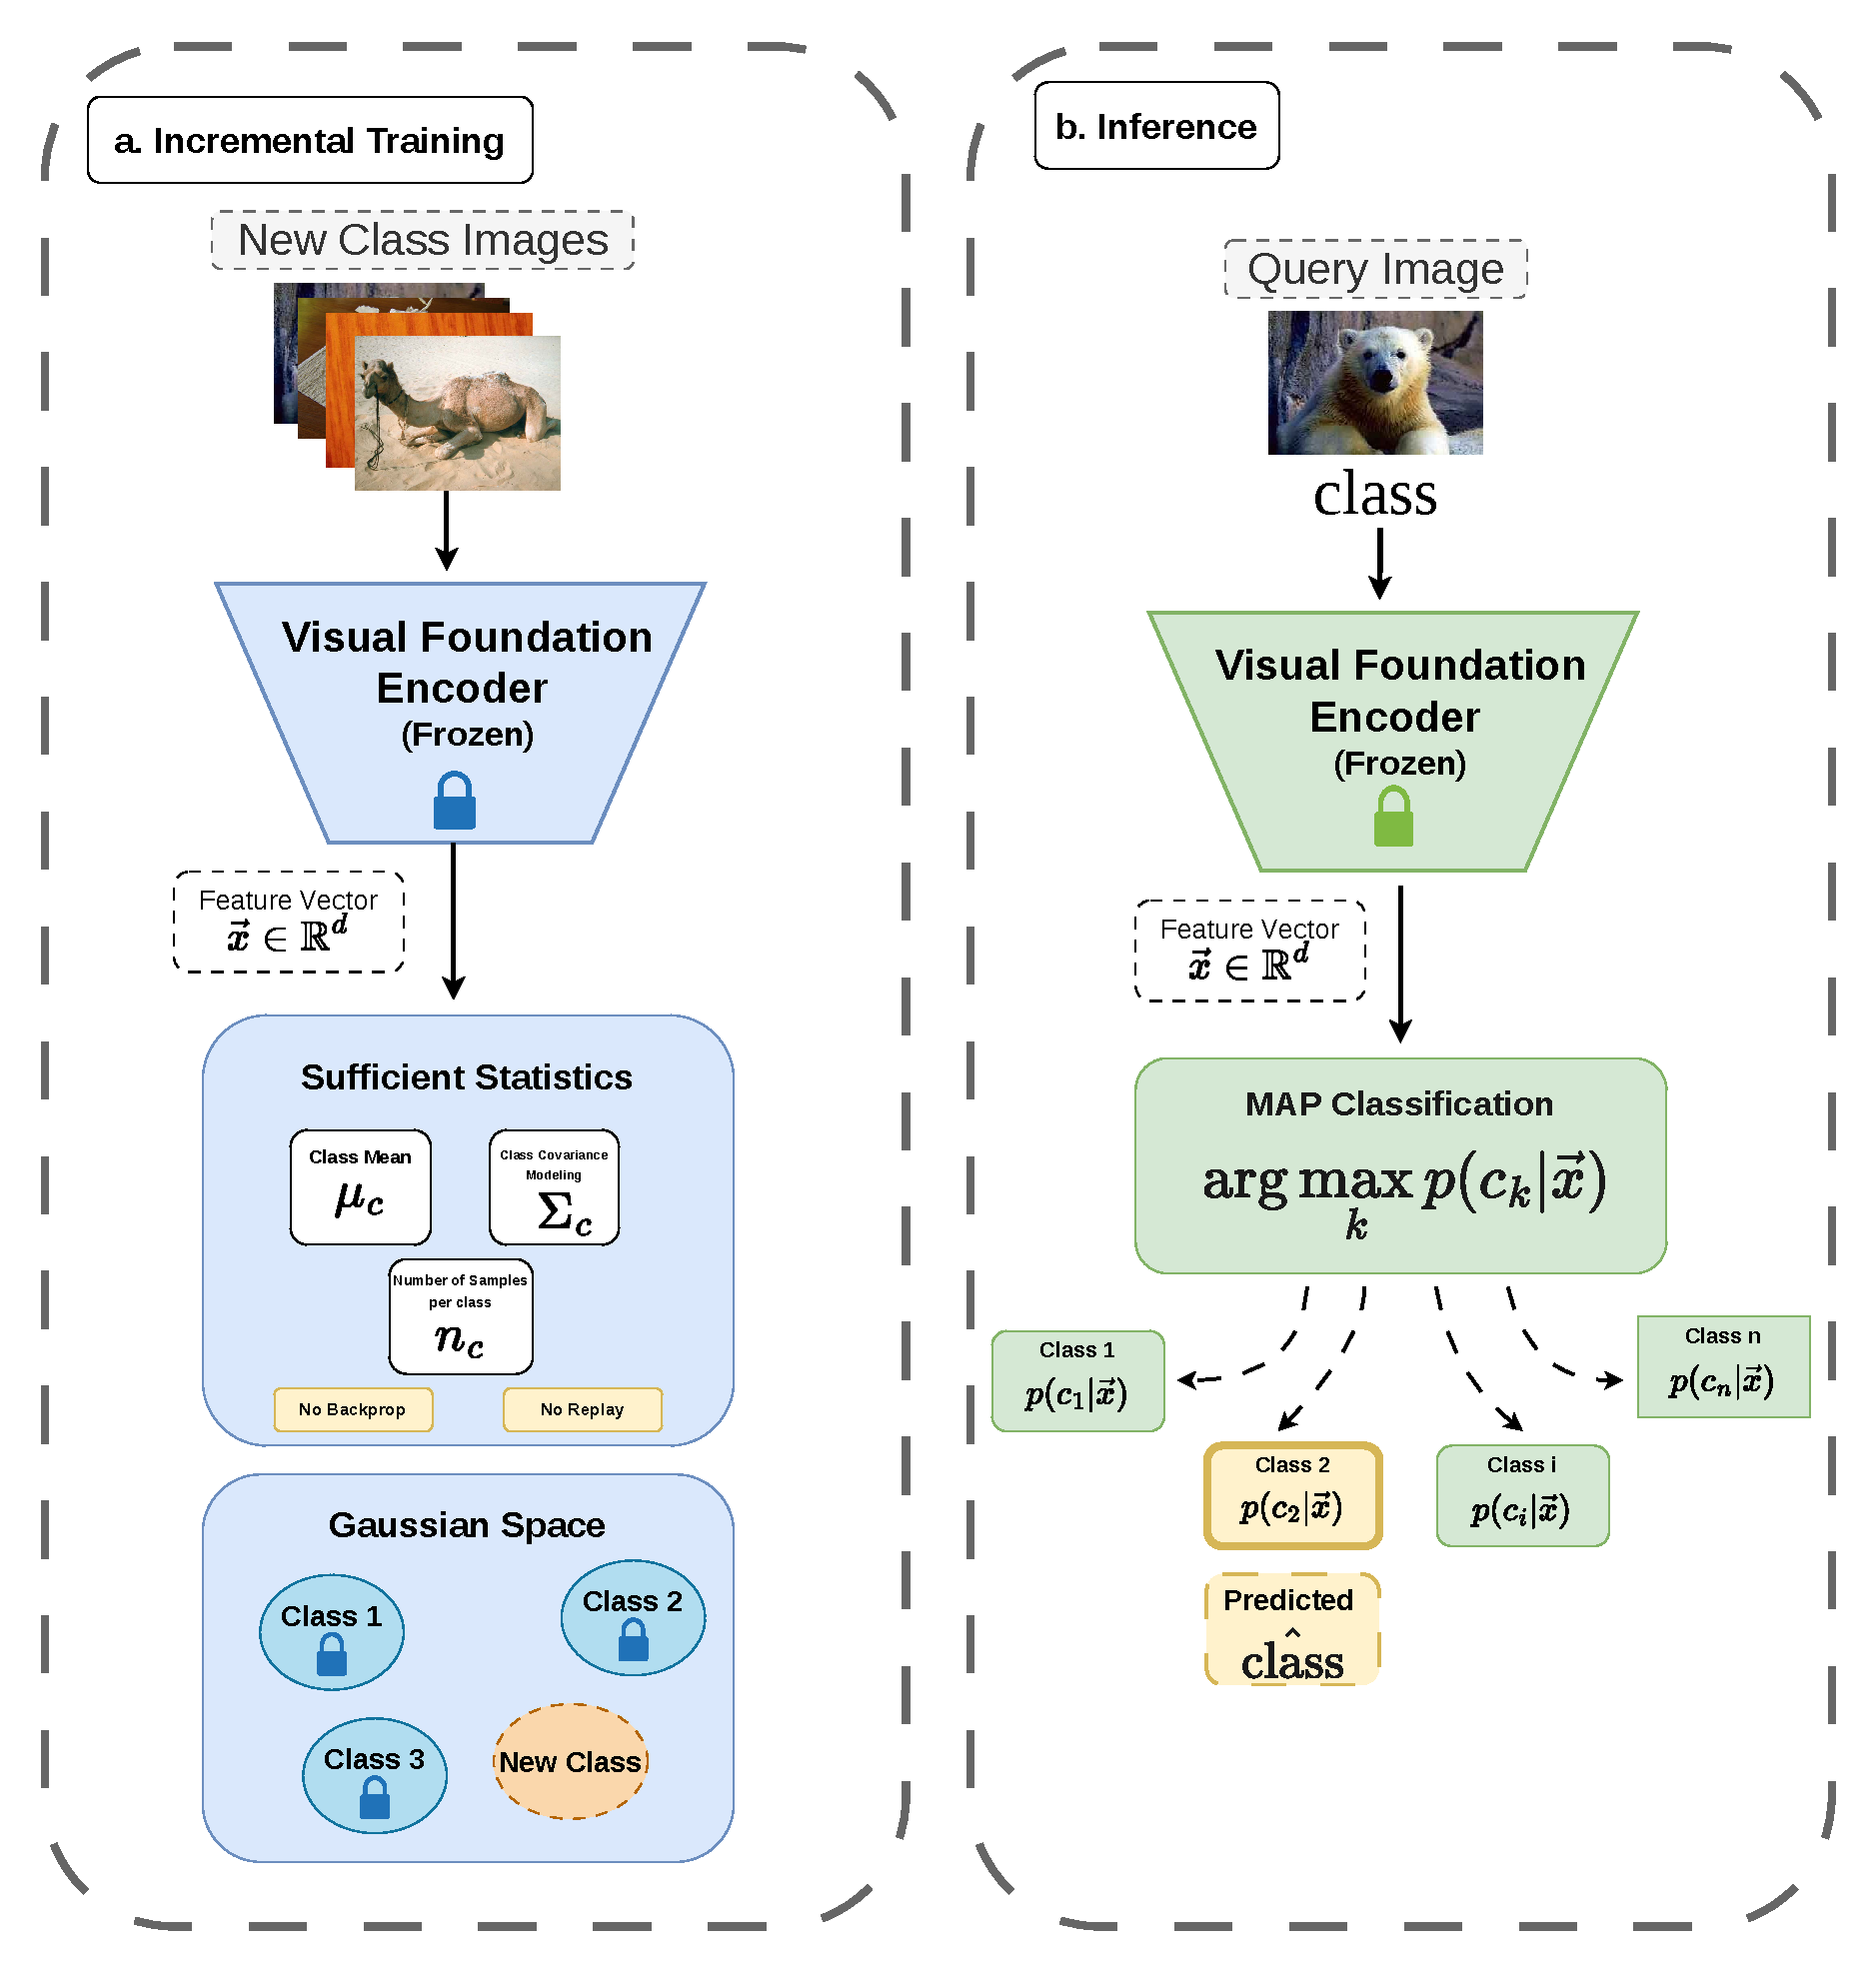
\includegraphics[width=0.6\textwidth]{imagenes/methodology/TMLR_block_diagram_approach.pdf}
	\caption{Overview of the proposed framework, reproduced from the peer-reviewed article that accompanies this thesis. A frozen foundation encoder maps each input image to a fixed embedding $\vec{x}\in\mathbb{R}^d$. Each class is represented by a Gaussian density (mean and covariance) that is updated incrementally without backpropagation. At inference, classification follows the MAP rule under the learned class-conditional densities. This diagram supersedes the general conceptual schematic used purely for narrative context in the Introduction (Figure~\ref{fig:intro_overview}), adding explicit detail on the recursive statistic-update mechanism shared by all covariance parameterisations introduced in Section~\ref{sec:covariance_estimation}.}
	\label{fig:architecture}
\end{figure}

\subsection{Likelihood-Based Classification}
\label{sec:method:classification}

Given an input image $x \in \mathcal{X}$, the frozen foundation model $\mathcal{F}$ produces a fixed-dimensional embedding
\begin{equation}
    \vec{x} = \mathcal{F}(x) \in \mathbb{R}^d
    \label{eq:feature_extractor}
\end{equation}
and all learning is performed directly in the stationary feature space $\mathbb{R}^d$. We adopt a generative modelling framework and assume class-conditional Gaussian feature distributions:
\begin{equation}
    p(\vec{x} \mid y = c) = \mathcal{N}(\vec{x} \mid \boldsymbol{\mu}_c,\, \boldsymbol{\Sigma}_c),
    \label{eq:class_gaussian}
\end{equation}
where $\boldsymbol{\mu}_c \in \mathbb{R}^d$ and $\boldsymbol{\Sigma}_c \succ 0$ are the class-specific mean and covariance matrix, estimated incrementally from observed samples. Classification is performed via Maximum A Posteriori (MAP) inference:
\begin{equation}
    \hat{y} = \arg\max_{c \in \mathcal{Y}} \left[ \log p(\vec{x} \mid y=c) + \log \pi_c \right],
    \label{eq:map}
\end{equation}
where $\pi_c = p(y=c)$ is the class prior. Under a uniform prior and the Gaussian density model, the decision rule is equivalent to the quadratic discriminant:
\begin{equation}
    \hat{y} = \arg\min_{c \in \mathcal{Y}} \left[ (\vec{x} - \boldsymbol{\mu}_c)^T \boldsymbol{\Sigma}_c^{-1} (\vec{x} - \boldsymbol{\mu}_c) + \log|\boldsymbol{\Sigma}_c| \right].
    \label{eq:qda}
\end{equation}
This quadratic decision function is the core of the proposed framework. The Mahalanobis term $(\vec{x}-\boldsymbol{\mu}_c)^T\boldsymbol{\Sigma}_c^{-1}(\vec{x}-\boldsymbol{\mu}_c)$ encodes the \emph{shape} of the class distribution while $\log|\boldsymbol{\Sigma}_c|$ encodes its \emph{volume}. The covariance parameterisations introduced in Section~\ref{sec:covariance_estimation} are specialisations of Equation~\eqref{eq:qda} that differ in the structure imposed on $\boldsymbol{\Sigma}_c$; the interplay between the shape and volume components is the central design axis of the covariance estimation study and is examined in detail in the analysis of results.

Adding a new class to the system requires only estimating the sufficient statistics $(\boldsymbol{\mu}_c, \boldsymbol{\Sigma}_c)$ in the fixed feature space; previously learned class statistics are never modified. This formulation therefore enables genuinely incremental updates without backpropagation, replay buffers, or exemplar storage.

\subsection{Datasets and Experimental Protocol}
We follow the standard Continual Learning (CL) protocol where the model learns a sequence of disjoint tasks and calculates the average accuracy and the forgetting. The four benchmarks used throughout this thesis are Split CIFAR-100, Split ImageNet-R, Split Caltech-256, and a heterogeneous Split Joint stream aggregating the three. The high-dimensional covariance estimators introduced in Section~\ref{sec:covariance_estimation} are stressed most heavily by the smallest of these per-class sample budgets, that of Split Caltech-256.

As mentioned, to quantify performance, SOTA works \cite{wang2022learning} utilize two standard metrics derived from the test accuracy scores: the average accuracy and the average forgetting.

With the architecture, benchmarks and evaluation metrics now in place, the remainder of this chapter follows a single, consistent narrative arc that Chapter~\ref{ch:results} mirrors section by section: it opens with the covariance-estimation methodology and its mixture-of-Gaussians extensions, then introduces the incremental class-inclusion protocol that stresses the growing decision surface, and closes with the sensitivity of the framework to the choice of upstream backbone. The feature-space characterization tools that these methodological choices rely on---the probabilistic confidence and calibration metrics, the inter-class pairwise Bhattacharyya and Euclidean distances, the spectral structure of the embedding space, and the statistical validation of the Gaussianity assumption on which the whole framework rests---are developed together in Chapter~\ref{ch:gaussian_space}.

\section{Covariance Estimation}
\label{sec:covariance_estimation}

Due to the high dimensionality of the extracted feature ($\vec{x}\in \mathbb{R}^d$), the empirical sample covariance matrix (SCM) is a poor estimator for each class: its eigenvalues are biased, and the matrix is singular whenever $n_c < d$. In our setting $d = 768$ while $n_c$ ranges from approximately $40$ to $400$ depending on the benchmark, so the matrix always has at most $n_c - 1$ non-zero eigenvalues out of $d = 768$, leaving $d - (n_c - 1)$ eigenvalues that are structurally zero before any regularisation is applied.
The Gaussian modelling assumption that motivates the covariance-based classifiers introduced below is formally validated later in Section~\ref{sec:method:gaussianity_main}; here we focus on how to obtain a well-conditioned covariance estimate under that assumption. Our benchmarks are tested using different covariance estimation methods:

\subsection{Diagonal Covariances}
In this configuration, we assume that the features within each class $c$ are independent, leading to a diagonal covariance matrix $\boldsymbol{\Sigma}_c = \text{diag}(\sigma_{c,1}^2, \sigma_{c,2}^2, \dots, \sigma_{c,d}^2)$. This simplification significantly reduces the number of parameters to estimate from $O(d^2)$ to $O(d)$, which is particularly advantageous when the dimensionality $d = 768$ is large relative to the number of samples per class. For each class $c \in \{1, \dots, C\}$, the mean vector $\boldsymbol{\mu}_c$ and the diagonal elements of $\boldsymbol{\Sigma}_c$ are computed as:

\begin{equation}
	\boldsymbol{\mu}_c = \frac{1}{n_c} \sum_{i=1}^{n_c} \vec{x}_i, \quad \sigma_{c,j}^2 = \frac{1}{n_c-1} \sum_{i=1}^{n_c} (x_{i,j} - \mu_{c,j})^2 + \epsilon
\end{equation}
where $\epsilon = 10^{-6}$ is a small constant added to ensure numerical stability and strictly positive variances. The log-likelihood of a test sample $\vec{x}$ belonging to class $c$ is determined by the discriminant function:

\begin{equation}
	g_c(\vec{x}) = \ln P(\vec{x}|c) + \ln P(c)
\end{equation}

Under the assumption of a uniform prior $P(c)$ and Gaussian distribution, this simplifies to:

\begin{equation}
	g_c(\vec{x}) = -\frac{1}{2} \sum_{j=1}^{d} \left( \ln(2\pi\sigma_{c,j}^2) + \frac{(x_j - \mu_{c,j})^2}{\sigma_{c,j}^2} \right)
\end{equation}


\subsection{Full Covariances}
\label{sec:method:full_cov}

To account for the dependencies between different dimensions of the feature vector, we estimate a full covariance matrix $\boldsymbol{\Sigma}_c \in \mathbb{R}^{d \times d}$ for each class $c$. While this provides a richer representation of the class distribution, the estimation of $d^2$ parameters is prone to ill-conditioning when the number of samples $n_c$ is limited.The mean vector $\boldsymbol{\mu}_c$ and the empirical covariance $\boldsymbol{\Sigma}_c$ are calculated as:

\begin{equation}
	\boldsymbol{\mu}_c = \frac{1}{n_c} \sum_{i=1}^{n_c} \vec{x}_i, \quad \boldsymbol{\Sigma}_c = \frac{1}{n_c - 1} \sum_{i=1}^{n_c} (\vec{x}_i - \boldsymbol{\mu}_c)(\vec{x}_i - \boldsymbol{\mu}_c)^T
\end{equation}

To ensure that the matrix is invertible and to improve numerical stability, a regularization is applied by adding a small identity term to the diagonal: $\hat{\boldsymbol{\Sigma}}_c = \boldsymbol{\Sigma}_c + \epsilon I$, with $\epsilon = 10^{-6}$.

For obtaining the precision matrix $Q_c$ (the inverse of the covariance matrix $\hat{\boldsymbol{\Sigma}}_c$), an approach based on Cholesky decompositions is used. The covariance $\hat{\boldsymbol{\Sigma}}_c$ is decomposed as
\begin{equation}
	\hat{\boldsymbol{\Sigma}}_c = C_c C_c^T, \qquad C_c L_c = I,
	\label{eq:cholesky_decomp}
\end{equation}
with $C_c$ lower triangular and $I$ the identity, so that $L_c = C_c^{-1}$ is the Cholesky factor of the precision matrix $Q_c = L_c^T L_c$.

Then, the squared Mahalanobis distance and the log-determinant are computed from $\boldsymbol{\mu}_c$ and $L_c$ as:

\begin{equation}
	d_M(\vec{x}, \boldsymbol{\mu}_c, L_c) = (\vec{x} L_c - \boldsymbol{\mu}_c L_c)^T (\vec{x} L_c - \boldsymbol{\mu}_c L_c)
	\label{eq:cholesky_mahalanobis}
\end{equation}

\begin{equation}
	\ln |\hat{\boldsymbol{\Sigma}}_c| = 2 \sum_{i=1}^{d}{\ln(L_{c \, i,i})}
	\label{eq:cholesky_logdet}
\end{equation}

\subsection{Hybrid Covariance}
\label{sec:method:hybrid_cov}

The hybrid covariance estimator decouples the squared Mahalanobis distance from its associated normalisation constant. For each class $c$, the full covariance matrix $\hat{\boldsymbol{\Sigma}}_c$ is estimated and regularised exactly as in Section~\ref{sec:method:full_cov}, and the squared Mahalanobis distance $d_M(\vec{x}, \mu_c, L_c)$ is computed using the same Cholesky-based procedure of Equations~\eqref{eq:cholesky_decomp}--\eqref{eq:cholesky_mahalanobis}, so that the \emph{shape} of the discriminant retains the full off-diagonal structure of the empirical covariance. However, the log-determinant term---which represents the \emph{volume} of the distribution---is computed using only the diagonal elements (variances) of the covariance matrix:
\begin{equation}
	\ln |\hat{\boldsymbol{\Sigma}}_c|_{\text{diag}} = \sum_{j=1}^{d} \ln(\sigma_{c,j}^2),
	\label{eq:hybrid_logdet}
\end{equation}
where $\sigma_{c,j}^2$ denotes the $j$-th diagonal entry of $\hat{\boldsymbol{\Sigma}}_c$. The resulting discriminant function is defined as:
\begin{equation}
	g_c(\vec{x}) = -\frac{1}{2} \left( d \ln(2\pi) + \sum_{j=1}^{d} \ln(\sigma_{c,j}^2) + d_M(\vec{x}, \boldsymbol{\mu}_c, L_c) \right).
	\label{eq:hybrid_discriminant}
\end{equation}

This formulation avoids the numerical issues that arise when near-zero eigenvalues of $\hat{\boldsymbol{\Sigma}}_c$ artificially inflate or destabilise the exact log-determinant, at the cost of using a diagonal approximation for the volume term only.

\subsection{OAS Covariance}
\label{sec:method:oas}

Oracle Approximating Shrinkage (OAS) is a shrinkage technique that computes an structurally optimized covariance matrix by finding an optimal compromise between the sample covariance matrix and a structured target (the identity matrix scaled by the average trace).The OAS estimator provides a more accurate estimation of the covariance $\boldsymbol{\Sigma}_c$ by minimizing the Mean Squared Error (MSE) under the assumption of Gaussianity. The estimated covariance is defined as:

\begin{equation}
	\hat{\boldsymbol{\Sigma}}_{\text{OAS}, c} = (1 - \rho_c) \hat{\boldsymbol{\Sigma}}_{\text{SCM}, c} + \rho_c \hat{F}_c
\end{equation}
where $\rho_c$ is the shrinkage coefficient calculated specifically for class $c$, $\hat{\boldsymbol{\Sigma}}_{\text{SCM}, c}$ is the sample covariance matrix, and $\hat{F}_c = \frac{\text{tr}(\hat{\boldsymbol{\Sigma}}_{\text{SCM}, c})}{d} I$ is the shrinkage target.In our implementation, we compute the precision matrix $\Psi_c = \hat{\boldsymbol{\Sigma}}_{\text{OAS}, c}^{-1}$ directly via the OAS algorithm. This precision matrix is then used to calculate the Mahalanobis distance in the log-likelihood discriminant function:

\begin{equation}
	g_c(\vec{x}) = \ln A_c - \frac{1}{2} (\vec{x} - \boldsymbol{\mu}_c)^T \Psi_c (\vec{x} - \boldsymbol{\mu}_c)
\end{equation}

where $\ln A_c$ is the normalization constant derived from the log-determinant of the OAS-estimated covariance matrix, evaluated numerically via the stable log-determinant of the eigendecomposition. This approach ensures that the model captures class-specific correlations while remaining robust to the ``curse of dimensionality.''

\subsection{Ledoit-Wolff}
\label{sec:method:ledoitwolf}

The Ledoit-Wolf Diagonal Anchor estimator addresses the instability of the sample covariance matrix $S$ by shrinking it toward a target matrix $T$.

The selection of a target matrix $T$ represents a prior assumption regarding the feature distribution. Both methods stabilize the estimator by pulling the noisy off-diagonal elements of the sample covariance matrix $S$ toward zero, but they differ in how they treat the diagonal elements (the variances).

\subsubsection{Diagonal Target}
The diagonal anchor is defined as $T_{\text{diag}} = \text{diag}(s_{11}, s_{22}, \dots, s_{dd})$. This approach assumes that the features are independent but allows for heteroscedasticity, meaning each dimension can have a different variance. Shrinkage toward this target preserves the scale of each individual feature as observed in the sample data while suppressing only the correlations. This is particularly useful when certain dimensions of the DINOv2 embeddings are naturally more informative or volatile than others.

\subsubsection{Identity Target}The identity anchor is more restrictive, defined as $T_{\text{ident}} = \mu I$, where $\mu = \frac{1}{d} \text{tr}(S)$ is the average variance across all dimensions. This target assumes that the features are not only independent but also share a common variance (homoscedasticity). The resulting distribution is spherical. Because the embeddings used in this work are L2-normalized, the variances across dimensions tend to be similar, making the identity anchor a highly robust regularizer that prevents any single dimension from disproportionately influencing the distance metric.

\subsubsection{Structural Summary}The fundamental difference between these two estimators lies in the flexibility of the variance components:

\begin{itemize}
	\item \textbf{Diagonal Anchor:} $\hat{\Sigma}_{ij} = (1-\gamma)s_{ij}$ for $i \neq j$, and $\hat{\Sigma}_{ii} = s_{ii}$. It yields an axis-aligned ellipsoidal distribution.
	\item \textbf{Identity Anchor:} $\hat{\Sigma}_{ij} = (1-\gamma)s_{ij}$ for $i \neq j$, and $\hat{\Sigma}_{ii} = (1-\gamma)s_{ii} + \gamma \mu$. It yields a distribution that is pulled toward a perfectly spherical geometry.
\end{itemize}

\subsection{Shared Covariance}
\label{subsec:shared_cov_original}

The Shared Covariance framework assumes that the internal noise or feature variability is homoscedastic across all classes. In this paradigm, all classes share a single covariance matrix $\boldsymbol{\Sigma}$, which captures the global structure of the feature space.

A key aspect of this framework in the continual learning setting is that $\boldsymbol{\Sigma}$ is re-estimated at the end of each task $t$ using only the classes observed so far, $\mathcal{C}_t = \{1, \dots, C_t\}$.

\section{Mixture of Gaussians}

In order to capture potential multi-modality within the feature space of a single class, we employ Gaussian Mixture Models (GMM). We implemented the following models using the previously defined diagonal, full and hybrid covariances approaches.

\subsection{Mixture of 2 Gaussians}

Forcing each class to be defined as a GMM with $K=2$ components, each class $c$ can be modeled by a probability density function:

\begin{equation}
	p(\vec{x}|c) = \sum_{k=1}^{K} \pi_{c,k} \mathcal{N}(\vec{x} | \boldsymbol{\mu}_{c,k}, \boldsymbol{\Sigma}_{c,k})
\end{equation}

where $\pi_{c,k}$ represents the mixing weight of the $k$-th component for class $c$, subject to $\sum \pi_{c,k} = 1$. In this specific variant, the covariance matrices $\boldsymbol{\Sigma}_{c,k}$ are restricted to be diagonal to maintain computational efficiency and prevent over-fitting in the high-dimensional DINOv2 space.The parameters $\{\pi_{c,k}, \boldsymbol{\mu}_{c,k}, \boldsymbol{\Sigma}_{c,k}\}$ are estimated using the Expectation-Maximization (EM) algorithm. To ensure numerical stability, a small constant $\epsilon = 10^{-5}$ is added to the diagonal of each covariance matrix. The log-likelihood for a test sample $\vec{x}$ is calculated using the \textit{LogSumExp} operator to avoid underflow:

\begin{equation}
	\ln p(\vec{x}|c) = \text{lnaddexp} \left( \ln(\pi_{c,1} \mathcal{N}(\vec{x} | \boldsymbol{\mu}_{c,1}, \boldsymbol{\Sigma}_{c,1})), \ln(\pi_{c,2} \mathcal{N}(\vec{x} | \boldsymbol{\mu}_{c,2}, \boldsymbol{\Sigma}_{c,2})) \right)
\end{equation}

In the implementation, this is expanded as:

\begin{equation}
	\ln p(\vec{x}|c) = \ln \left( \exp( \ln \pi_{c,1} + \ln A_{c,1} - \frac{1}{2} d_{M,1} ) + \exp( \ln \pi_{c,2} + \ln A_{c,2} - \frac{1}{2} d_{M,2} ) \right)
\end{equation}

where $d_{M,k}$ is the diagonal Mahalanobis distance to the $k$-th component and $\ln A_{c,k}$ is the normalization constant. This approach allows the model to better represent classes that may contain significantly different visual sub-types or clusters within the latent embedding space.


\subsection{Mixture of up-to-4 Gaussians}

To adapt to the varying complexity of different classes within the different datasets, we implement a flexible Gaussian Mixture Model where the number of components $K_c$ for each class $c$ is not fixed. Instead, the model selects the most appropriate number of components $K_c \in \{1, 2, 3, 4\}$ by minimizing the Bayesian Information Criterion (BIC).The BIC is defined as:

\begin{equation}
	\text{BIC} = \ln(n)k - 2\ln(\hat{L})
	\label{eq:bic_mog4}
\end{equation}

where $n$ is the number of samples in the class, $k$ is the number of free parameters to be estimated, and $\hat{L}$ is the maximized value of the likelihood function. By using diagonal covariance matrices, the number of parameters per component is kept low ($2d + 1$), allowing the selection process to favor multi-modal distributions only when the increase in likelihood justifies the additional parameters. For each component $k$ in class $c$, the diagonal covariance $\boldsymbol{\Sigma}_{c,k} = \text{diag}(\sigma_{c,k,1}^2, \dots, \sigma_{c,k,d}^2)$ is regularized with $\epsilon = 10^{-6}$. The classification of a test sample $\vec{x}$ involves calculating the weighted log-likelihood across all active classes:

\begin{equation}
	\ln p(\vec{x}|c) = \text{LSE}_{k=1}^{K_c} \left( \ln \pi_{c,k} - \frac{1}{2} \left( \sum_{j=1}^{d} \ln(2\pi\sigma_{c,k,j}^2) + \sum_{j=1}^{d} \frac{(x_j - \mu_{c,k,j})^2}{\sigma_{c,k,j}^2} \right) \right)
\end{equation}

where $\text{LSE}$ denotes the LogSumExp operator. This methodology allows for a more granular representation of class distributions—using a single Gaussian for simple, compact classes and up to four Gaussians for classes with high intra-class variance or distinct visual sub-clusters—while preserving the numerical efficiency of diagonal estimators.

\section{Incremental Class Inclusion}
\label{sec:method:incremental}

Having defined the full family of covariance estimators in Section~\ref{sec:covariance_estimation}, we design a class-incremental evaluation protocol to systematically assess how each closed-form estimator scales as the overall classification task grows in complexity. Rather than measuring conventional catastrophic forgetting—given that each class-conditional Gaussian is estimated independently and frozen upon initialization—this incremental class inclusion experiment isolates the impact of a progressively hardening decision surface on classification performance. By sequentially expanding the set of active classes and tracking the evolution of average accuracy over the growing pool of target categories, we can observe how the physical expansion of the label space translates into geometric crowding within the underlying feature space. This experimental design directly bridges empirical performance degradation with the architectural geometry of the learned representations, paving the way to quantify how the introduction of new class-conditional distributions compresses the margins between prototype boundaries and intensifies pairwise class confusion.


\section{Backbones Comparison}
\label{sec:method:backbones}

Throughout this work, DINOv2 \cite{oquab2024dinov} is used as the default backbone feature extractor for the Gaussian-based classifiers because of its self-supervised training regime and the strong empirical evidence of approximately Gaussian, well-conditioned class-conditional distributions presented in Section~\ref{sec:method:gaussianity_main}. However, the proposed framework is agnostic to the specific feature extractor used: any frozen encoder that produces fixed-dimensional embeddings can plug in unchanged into the downstream Gaussian classifier. To quantify the dependence of the framework on the choice of backbone, we further analyse the impact of the backbone architecture by re-running the Diag-Cov and Full-Cov variants using two supervised Vision Transformers from the \texttt{timm} library \cite{rw2019timm}: \textbf{ViT-base/16} (ViT-b, $d=768$) and \textbf{ViT-medium/16} (ViT-m, $d=512$), both pre-trained on ImageNet-21k \cite{imagenet21k}. The covariance estimation, hyper-parameters and evaluation protocol are kept identical across backbones to isolate the effect of the upstream representation; the results are reported in Section~\ref{sec:backbone_results}.

This concludes the description of the proposed methodology: the frozen-backbone Gaussian architecture, the covariance-estimation family and its mixture-of-Gaussians extensions, the incremental class-inclusion protocol, and the backbone-sensitivity ablation. Chapter~\ref{ch:gaussian_space} develops, in a single consolidated treatment, the mathematical and statistical tools---spectral analysis, Gaussianity testing, inter-class separability, and confidence calibration---used to characterize the feature space these methods operate on, before Chapter~\ref{ch:results} reports and interprets the resulting empirical evidence.

\chapter{Experimental Results and Analysis}
\label{ch:results}
\label{ch:analysis}

This chapter presents the quantitative results of the experiments carried out in this thesis, together with their interpretation, topic by topic. It opens by presenting the benchmarks used throughout the thesis and formally defining the metrics computed over them, both the average accuracy and forgetting scores and the complementary confidence and calibration metrics. From there, the covariance estimators and mixture-of-Gaussian variants results are presented, then how well-calibrated their predictions actually are, then how the system behaves as more classes are added over time, and how separable classes are from one another in the embedding space. It then looks at the feature space itself---its sensitivity to the choice of backbone, its spectral structure, and how well it satisfies the Gaussianity assumption the whole framework rests on---and closes by weighing the computational cost of the framework before summarising the practical conclusions that follow from all of this evidence taken together.

Before going further, it is worth fixing the short names used repeatedly in the tables and discussion below. \textbf{Diag-Cov} and \textbf{Full-Cov} are the two basic covariance parameterisations introduced in Section~\ref{sec:covariance_estimation}: a diagonal covariance matrix, which treats feature dimensions as independent of one another, and a full covariance matrix, which also captures the correlations between them. \textbf{Hybrid-Cov} is the intermediate estimator that keeps the full covariance structure for the Mahalanobis, shape-related term of the discriminant, while using only its diagonal for the log-determinant, volume-related term. \textbf{OAS} and \textbf{LW-I}/\textbf{LW-D} are the two shrinkage-based estimators introduced in the same section: Oracle Approximating Shrinkage, and Ledoit--Wolf shrinkage toward an Identity or a Diagonal target, respectively. The prefix \textbf{Shared-} (as in Shared-Diag-Cov or Shared-Full-Cov) means that the corresponding covariance is estimated once, globally, and reused across every class, rather than independently per class. Finally, \textbf{MOG2} and \textbf{MOG4} denote mixture-of-Gaussian variants with exactly two, or with up to four, components per class, respectively; the trailing letter---\textbf{D}, \textbf{F}, or \textbf{H}---again indicates whether each individual component uses a diagonal, full, or hybrid covariance, and \textbf{MOG4-Shared} combines the multi-component MOG4 formulation with a single, globally shared full-covariance matrix.

For every benchmark we report the average accuracy after the last task, $A_{T}$, and the forgetting score $F_{T}$, both formally defined below. Whenever possible we report mean and variance over three independent runs (different task-order seeds). Since the proposed Gaussian classifiers maintain only sufficient statistics $(\boldsymbol{\mu}_c, \boldsymbol{\Sigma}_c)$ and do not involve parameter optimisation during incremental updates, the resulting classifier is independent of the specific class-presentation order; this explains the $\pm 0.00$ standard deviation reported for our methods throughout. State-of-the-art prompt-based competitors are reproduced from the published values reported in their respective papers. Methods proposed in this thesis are highlighted in grey. The best result per column is shown in bold.

\section{Image Datasets and Benchmarks}
\label{sec:an:datasets}

Before reporting any empirical result, this section presents the four benchmarks evaluated throughout this thesis. We first introduce the underlying image datasets and what makes each one relevant to this work, and then explain how each one is turned into a class-incremental stream.

\subsection{Source Datasets}
\label{sec:an:source_datasets}

Three source datasets are used to build the benchmarks of this thesis, chosen so that, together, they vary in image resolution, visual style, and category granularity. \textbf{CIFAR-100} \cite{cifar100} contains 60,000 low-resolution ($32\times32$) natural images, organised into 100 ``fine'' classes grouped under 20 broader ``coarse'' categories. \textbf{Caltech-256} \cite{caltech256} contains 30,607 higher-resolution images spread across 256 categories, with more images per class and more visual diversity than CIFAR-100; in this thesis, we use its first 250 categories, for reasons explained below. \textbf{ImageNet-R} \cite{imagenetR} takes 200 of the classes from the original ImageNet \cite{imagenet} and replaces their photographs with 30,000 non-photographic renditions instead, such as paintings, cartoons, and sketches, which makes it well suited for testing robustness to this kind of stylistic domain shift. A fourth, much larger dataset, \textbf{ImageNet-21k} \cite{imagenet21k}, is not itself turned into a benchmark in this section, but is used elsewhere in this thesis as pre-training data, both for the backbones compared in Section~\ref{sec:backbone_results} and for the fixed projection matrix used in the PCA probe of Section~\ref{sec:spectral_analysis}.

\subsection{Continual Learning Splits and Protocol}
\label{sec:an:cl_splits}

Each of the three source datasets above is turned into a class-incremental benchmark by splitting its classes into a fixed sequence of disjoint tasks, following the standard protocol described in Chapter~\ref{methodology}: the model sees one task at a time, and average accuracy and forgetting, formally defined in Section~\ref{sec:an:metrics}, are computed over the classes seen so far. A fourth benchmark then combines all three streams into a single, longer one. Concretely:

\begin{itemize}
	\item \textbf{Split CIFAR-100} divides the 100 classes into 10 disjoint tasks of 10 classes each.

	\item \textbf{Split ImageNet-R} divides its 200 classes, randomly, into 10 tasks of 20 classes each; because its images are stylistic renditions rather than plain photographs, this split also introduces a deliberate domain-shift challenge on top of the usual class-incremental one.

	\item \textbf{Split Caltech-256} keeps only the first 250 of the original 256 categories, so that they divide evenly into 10 balanced tasks of 25 classes each (the remaining six categories are simply discarded). The resulting stream has around 28\,100 images and an average of $\overline{n_c}\!\approx\!112$ training samples per class, the smallest per-class budget of the three datasets, which makes it the one that puts the most pressure on the high-dimensional covariance estimators of Section~\ref{sec:covariance_estimation}.

	\item \textbf{Split Joint} concatenates the 30 tasks of the three benchmarks above into a single, heterogeneous, 30-task stream, presented to the model in a randomised order. This forces the classifier to move between natural, artistic, and high-resolution images within the same run, and is meant to stress-test the framework over a much longer and more varied stream than any of the three individual benchmarks alone.
\end{itemize}

\subsection{Benchmark Properties Summary}
\label{sec:an:benchmark_summary}

The four resulting benchmarks span a wide spectrum of statistical difficulty for a Gaussian classifier. Their salient properties are summarised in Table~\ref{tab:dataset_summary}.

\begin{table}[htbp]
	\centering
	\caption{Statistical characterisation of the four benchmarks. $\overline{n_c}$ denotes the average sample budget per class.}
	\label{tab:dataset_summary}
	\scriptsize
	\setlength{\tabcolsep}{4pt}
	\begin{tabular}{lcccccc}
		\toprule
		\textbf{Benchmark} & \textbf{\# Classes} & \textbf{\# Tasks} & \textbf{Image source} & $\overline{n_c}$\\
		\midrule
		Split CIFAR-100   & 100 & 10 & Natural, low-resolution ($32{\times}32$)   & $500$    \\
		Split ImageNet-R  & 200 & 10 & Renditions: art, sketch, cartoon          & $150$     \\
		Split Caltech-256 & 250 & 10 & Natural, high-resolution, variable scale  & $112$  \\
		Split Joint       & 550 & 30 & Heterogeneous concatenation of the above  & mixed    \\
		\bottomrule
	\end{tabular}
\end{table}

The three primary datasets differ along two largely orthogonal axes: visual complexity (which determines how heavy-tailed the embedding coordinates are) and sample budget (which determines how reliably the per-class covariance can be estimated). CIFAR-100 occupies the favourable corner of both axes, ImageNet-R adds a deliberate input-distribution shift, and Caltech-256 combines heavy tails with a small per-class budget. The Joint benchmark inherits the worst feature of each of the three constituent datasets and is therefore the most informative regime for separating method behaviour. With the benchmarks now fully characterised, we turn to the evaluation metrics computed over them.

\section{Evaluation Metrics: Average Accuracy and Forgetting}
\label{sec:an:metrics}

 As is common in the continual learning literature \cite{wang2022learning}, we quantify performance using two standard metrics derived from the test accuracy scores obtained after each task: the average accuracy and the average forgetting.

On the one hand, \textbf{Average Accuracy ($A_t$)}, presented on equation \eqref{eq_AA}, measures overall performance after task $t$. It is the mean test accuracy across all tasks learned up to that point.

\begin{equation}
	A_t = \frac{1}{t} \sum_{\tau=1}^{t} S_{t,\tau}
	\label{eq_AA}
\end{equation}

On the other hand, \textbf{Forgetting ($F_{t}$)}, presented on equation \eqref{eq_AF}, quantifies how much the model has forgotten earlier tasks. It computes, for each past task, how much accuracy has dropped compared to its best historical score, and averages those drops.

\begin{equation}
	F_t = \frac{1}{t-1} \sum_{\tau=1}^{t-1} \left( \max_{k \le t-1} S_{k,\tau} - S_{t,\tau} \right)
	\label{eq_AF}
\end{equation}

Regarding forgetting, the proposed framework does not exhibit forgetting in the conventional sense, as previously learned class statistics are never modified when new classes are introduced. The measured forgetting values therefore primarily reflect the increased classification difficulty as the number of competing classes grows, rather than degradation of previously learned representations.

\section{Confidence and Calibration Metrics}
\label{sec:an:calibration_metrics_def}

Accuracy and forgetting measure whether the model's predictions are correct, but they say nothing about whether the model's own confidence in those predictions can be trusted---a distinction that matters in particular for Class-Incremental Learning, where a classifier can look accurate while still being systematically over- or under-confident. To capture this, we introduce five complementary metrics that jointly characterise the probabilistic behaviour of the classifier: the Expected Calibration Error (ECE) measures the global alignment between confidence and accuracy; the Confidence on Errors (CoE) quantifies how dangerously overconfident the model is when it fails; Total Confidence (TC) and Probability Margin (PM) both capture the decisiveness of the posterior distribution from two complementary angles; and the Average Predictive Entropy ($H$) measures the spread of probability mass across all classes. These definitions are used directly in Section~\ref{sec:calibration_results_section}, where the resulting values are reported and interpreted.

\subsection{Expected Calibration Error (ECE)}
This metric quantifies the mismatch between predictive confidence and empirical accuracy. We partition the predictions into $M$ equally spaced bins based on their confidence scores. The ECE is defined as the weighted average of the absolute difference between the accuracy and confidence of each bin:

\begin{equation}
	ECE_t = \sum_{m=1}^{M} \frac{|B_m|}{N} \left| acc(B_m) - conf(B_m) \right|\label{eq_ECE}
\end{equation}

where $N$ is the total number of samples, $B_m$ is the set of indices of samples whose prediction confidence falls into the $m$-th interval, and $acc(B_m)$ and $conf(B_m)$ represent the mean accuracy and mean confidence within that bin, respectively.

\subsection{Confidence on Errors (CoE)}
To specifically analyze the model's behavior when it fails, we measure the average confidence assigned to the winning (but incorrect) class. High CoE indicates a model that is ``dangerously wrong'', which matters in safety-oriented applications. It is computed for a task $t$ as:

\begin{equation}
	CoE_t = \frac{1}{|\mathcal{E}_t|} \sum_{i \in \mathcal{E}_t} \max(\hat{p}_i)
\end{equation}

where $\mathcal{E}_t$ is the set of misclassified samples and $\hat{p}_i$ is the predicted probability distribution for sample $i$.

\subsection{Total Confidence (TC)}

Total Confidence measures how certain the model is on average about its top-1 prediction, regardless of whether that prediction is correct:

\begin{equation}
	TC_t = \frac{1}{N} \sum_{i=1}^{N} \max_{c} \, p_{i,c}
\end{equation}

A value of $TC=1$ means the model assigns all probability mass to a single class for every sample---it is always maximally decisive. A value close to $1/C$ would indicate near-uniform posteriors. TC is a measure of \emph{decisiveness}, not correctness: a well-calibrated model should have $TC \approx A_T$ (confident when right, uncertain when wrong), whereas a badly overconfident model can reach $TC \approx 1$ even at low accuracy.

\subsection{Probability Margin (PM)}

The Probability Margin is the natural, non-logarithmic measure of how decisively the model separates its top-1 prediction from its second-best alternative:

\begin{equation}
	PM_t = \frac{1}{N} \sum_{i=1}^{N} \Bigl( p_{i,(1)} - p_{i,(2)} \Bigr)
\end{equation}

where $p_{i,(1)} \ge p_{i,(2)}$ are the two highest posterior probabilities for sample $i$. A margin near $1$ means the model almost entirely ignores its second candidate; a margin near $0$ means the model is nearly tied between its top-two guesses and one should treat the prediction with caution. PM is bounded in $[0,1]$ and directly interpretable: a value of $0.7$ means the winning class is, on average, assigned $70\%$ more probability than the runner-up.

\subsection{Average Predictive Entropy ($H$)}
We utilize Shannon entropy to measure the uncertainty of the model's predictions. A higher entropy suggests that the model is distributing its probability mass across multiple classes, indicating lower certainty. For task $t$, the average entropy is calculated as:

\begin{equation}
	H_t = \frac{1}{N} \sum_{i=1}^{N} \left( - \sum_{c=1}^{C} p_{i,c} \log(p_{i,c}) \right)
\end{equation}

where $p_{i,c}$ is the probability assigned to class $c$ for sample $i$.

\subsection*{Summary of calibration and uncertainty metrics}

Table~\ref{tab:metrics_summary} collects all six metrics (accuracy and the five calibration/uncertainty indicators), their range, the direction of improvement, and the key question each one answers. Together they provide a multi-dimensional view of the model's reliability throughout continual learning: accuracy tells us \emph{how often} the model is right; ECE tells us \emph{how well-calibrated} its probabilities are; CoE tells us \emph{how dangerous} its mistakes are; TC tells us \emph{how decisive} it is overall; PM tells us \emph{how clearly} it separates its top-two candidates; and entropy tells us \emph{how spread} its uncertainty is across all classes.

\begin{table}[htb]
	\centering
	\caption{Summary of the probabilistic calibration and uncertainty metrics used in this work. ``Better'' indicates the direction of the preferred value; ``context'' means both high and low values are informative depending on whether predictions are correct.}
	\label{tab:metrics_summary}
	\scriptsize
	\setlength{\tabcolsep}{5pt}
	\renewcommand{\arraystretch}{1.25}
	\begin{tabular}{llcll}
		\toprule
		\textbf{Metric} & \textbf{Symbol} & \textbf{Range} & \textbf{Better} & \textbf{Key question} \\
		\midrule
		Accuracy                    & $A_T$  & $[0,1]$         & $\uparrow$   & What fraction of predictions are correct? \\
		Expected Calibration Error  & ECE    & $[0,1]$         & $\downarrow$ & How well does confidence match actual accuracy? \\
		Confidence on Errors        & CoE    & $[0,1]$         & $\downarrow$ & How confident is the model when it is \emph{wrong}? \\
		Total Confidence            & TC     & $[0,1]$         & context      & How decisive is the model on its top-1 choice? \\
		Probability Margin          & PM     & $[0,1]$         & context      & How much more likely is top-1 than top-2? \\
		Predictive Entropy          & $H$    & $[0, \log C]$   & $\downarrow$ & How spread is probability mass over all $C$ classes? \\
		\bottomrule
	\end{tabular}
\end{table}

With accuracy, forgetting, and the confidence and calibration metrics now all formally established, we turn to the empirical results themselves, beginning with the covariance estimators and mixture-of-Gaussian variants.

\section{Covariance Estimator and Mixture-of-Gaussian Results}

\label{sec:covariance_results}
Table~\ref{tab:combined_benchmarks} reports the average accuracy and the forgetting score for every covariance estimator (diagonal, full, hybrid, Ledoit--Wolf identity/diagonal target~\cite{Ledoit2004}, OAS~\cite{Chen2010}) and for the mixture-of-Gaussian variants MOG-$k$ with $k\in\{2,4\}$ components and three sub-variants (\textit{D}, \textit{F}, \textit{H} for diagonal, full and hybrid covariance respectively). 
To ensure statistical robustness, all proposed configurations are evaluated across three independent experimental runs using distinct randomized task-presentation seeds, with performance reported as the sample mean alongside its corresponding standard deviation. For the state-of-the-art baselines, these variance metrics are included when available from their original literature sources.
The table is organised in three blocks: prompt-based state-of-the-art baselines reproduced from the literature (L2P, DualPrompt, APT); analytic, feature-based baselines (SimpleCIL, FeCAM, RanPAC); and, at the bottom, the proposed Gaussian estimators. Table~\ref{tab:split_joint} reports the same family on the 30-task Joint stream.

\begin{table}[htb]
	\centering
	\caption{Continual-learning performance on the three 10-task benchmarks. $A_{10}$ and $F_{10}$ are reported in percentage points.}
	\label{tab:combined_benchmarks}
	\scriptsize
	\begin{tabularx}{\textwidth}{lXXXXXX}
		\toprule
		\textbf{Method} & \multicolumn{2}{c}{\textbf{Split CIFAR-100}} & \multicolumn{2}{c}{\textbf{Split ImageNet-R}} & \multicolumn{2}{c}{\textbf{Split Caltech-256}} \\
		\cmidrule(lr){2-3} \cmidrule(lr){4-5} \cmidrule(lr){6-7}
		& \multicolumn{1}{c}{$A_{10} (\uparrow)$} & \multicolumn{1}{c}{$F_{10} (\downarrow)$} & \multicolumn{1}{c}{$A_{10} (\uparrow)$} & \multicolumn{1}{c}{$F_{10} (\downarrow)$} & \multicolumn{1}{c}{$A_{10} (\uparrow)$} & \multicolumn{1}{c}{$F_{10} (\downarrow)$} \\
		\midrule
		L2P             & $83.86 \pm 1.17$ & $7.35 \pm 0.39$ & $61.57 \pm 0.40$ & $9.73 \pm 0.42$ & $92.11 \pm 0.32$ & $2.94 \pm 0.26$ \\
		DualPrompt      & $86.51 \pm 0.49$ & $5.16 \pm 0.20$ & $68.13 \pm 0.52$ & $4.68 \pm 0.18$ & $92.50 \pm 0.16$ & $2.50 \pm 0.16$ \\
		DualPrompt-PGP  & $86.92 \pm 0.05$ & $5.35 \pm 0.19$ & $69.34 \pm 0.05$ & $4.53 \pm 0.04$ & \multicolumn{1}{c}{---} & \multicolumn{1}{c}{---} \\
		CODA-Prompt     & $87.00 \pm 0.38$ & $4.78 \pm 0.24$ & $74.24 \pm 0.56$ & $4.92 \pm 0.21$ & \multicolumn{1}{c}{---} & \multicolumn{1}{c}{---} \\
		CPrompt         & $87.83 \pm 0.37$ & $4.88 \pm 0.79$ & $76.71 \pm 0.61$ & $4.66 \pm 0.93$ & \multicolumn{1}{c}{---} & \multicolumn{1}{c}{---} \\
		ConvPrompt      & $88.87 \pm 0.33$ & $4.75 \pm 0.15$ & $77.86 \pm 0.25$ & $4.33 \pm 0.24$ & \multicolumn{1}{c}{---} & \multicolumn{1}{c}{---} \\
		RainbowPrompt   & $89.86 \pm 0.11$ & $3.44 \pm 0.26$ & $79.09 \pm 0.13$ & $3.90 \pm 0.23$ & \multicolumn{1}{c}{---} & \multicolumn{1}{c}{---} \\
		APT             & $88.88 \pm 0.65$ & $3.47 \pm 0.55$ & $79.40 \pm 0.47$ & $3.47 \pm 0.55$ & \multicolumn{1}{c}{---} & \multicolumn{1}{c}{---} \\
		\midrule
		SimpleCIL (NMC) \cite{janson2022simple} & $83.70$ & \multicolumn{1}{c}{---} & $55.56$ & \multicolumn{1}{c}{---} & \multicolumn{1}{c}{---} & \multicolumn{1}{c}{---} \\
		FeCAM \cite{goswami2024fecam}           & $85.70$ & \multicolumn{1}{c}{---} & $63.70$ & \multicolumn{1}{c}{---} & \multicolumn{1}{c}{---} & \multicolumn{1}{c}{---} \\
		RanPAC \cite{mcdonnell2023ranpac}       & $\mathbf{92.20}$ & \multicolumn{1}{c}{---} & $77.90$ & \multicolumn{1}{c}{---} & \multicolumn{1}{c}{---} & \multicolumn{1}{c}{---} \\
		\midrule
		\rowcolor{gray!15} Diag-Cov (ours)         & $86.07 \pm 0.00$ & $4.30 \pm 0.12$ & $77.12 \pm 0.00$ & $7.44 \pm 0.17$ & $90.06 \pm 0.00$ & $1.69 \pm 0.36$ \\
		\rowcolor{gray!15} Full-Cov (ours)         & $88.38 \pm 0.00$ & $4.12 \pm 0.00$ & $74.71 \pm 0.00$ & $5.16 \pm 0.02$ & $94.93 \pm 0.01$ & $1.74 \pm 0.05$ \\
		\rowcolor{gray!15} Hybrid-Cov (ours)       & $88.38 \pm 0.00$ & $4.18 \pm 0.00$ & $74.71 \pm 0.00$ & $5.03 \pm 0.04$ & $94.93 \pm 0.00$ & $2.09 \pm 0.08$ \\
		\rowcolor{gray!15} Shared-Diag-Cov (ours)  & $86.87 \pm 0.00$ & $4.72 \pm 0.17$ & $75.40 \pm 0.00$ & $5.17 \pm 0.38$ & $92.97 \pm 0.00$ & $2.06 \pm 0.02$ \\
		\rowcolor{gray!15} Shared-Full-Cov (ours)  & $88.72 \pm 0.00$ & $4.68 \pm 0.16$ & $77.99 \pm 0.00$ & $5.87 \pm 1.44$ & $93.62 \pm 0.00$ & $2.39 \pm 0.09$ \\
		\rowcolor{gray!15} MOG2-D (ours)           & $86.96 \pm 0.00$ & $4.24 \pm 0.02$ & $70.15 \pm 0.00$ & $4.93 \pm 0.02$ & $91.41 \pm 0.00$ & $1.67 \pm 0.30$ \\
		\rowcolor{gray!15} MOG2-F (ours)           & $85.01 \pm 0.00$ & $5.13 \pm 0.17$ & $73.42 \pm 0.00$ & $5.49 \pm 0.26$ & $93.95 \pm 0.00$ & $2.14 \pm 0.11$ \\
		\rowcolor{gray!15} MOG2-H (ours)           & $84.68 \pm 0.00$ & $5.26 \pm 0.22$ & $73.52 \pm 0.00$ & $5.47 \pm 0.23$ & $93.93 \pm 0.00$ & $2.13 \pm 0.10$ \\
		\rowcolor{gray!15} MOG4-D (ours)           & $87.80 \pm 0.00$ & $4.02 \pm 0.06$ & $72.52 \pm 0.01$ & $5.06 \pm 0.15$ & $91.12 \pm 0.00$ & $1.63 \pm 0.31$ \\
		\rowcolor{gray!15} MOG4-F (ours)           & $88.87 \pm 0.00$ & $3.99 \pm 0.00$ & $75.07 \pm 0.00$ & $5.07 \pm 0.05$ & $94.39 \pm 0.00$ & $2.12 \pm 0.08$ \\
		\rowcolor{gray!15} MOG4-H (ours)           & $88.88 \pm 0.00$ & $4.04 \pm 0.00$ & $75.01 \pm 0.00$ & $5.12 \pm 0.04$ & $94.36 \pm 0.00$ & $2.09 \pm 0.08$ \\
		\rowcolor{gray!15} MOG4-Shared (ours)      & $88.98 \pm 0.00$ & $4.03 \pm 0.09$ & $\mathbf{80.19 \pm 0.00}$ & $4.44 \pm 0.12$ & $\mathbf{94.61 \pm 0.00}$ & $1.88 \pm 0.09$ \\
		\rowcolor{gray!15} OAS (ours)              & $84.38 \pm 0.00$ & $3.90 \pm 0.07$ & $71.47 \pm 0.00$ & $4.57 \pm 0.29$ & $86.70 \pm 0.00$ & $1.90 \pm 1.77$ \\
		\rowcolor{gray!15} LW-I (ours)             & $84.78 \pm 0.00$ & $3.93 \pm 0.09$ & $71.91 \pm 0.00$ & $4.54 \pm 0.43$ & $89.89 \pm 0.00$ & $1.50 \pm 0.08$ \\
		\rowcolor{gray!15} LW-D (ours)             & $82.85 \pm 0.00$ & $3.94 \pm 0.28$ & $70.35 \pm 0.00$ & $4.62 \pm 0.95$ & $90.04 \pm 0.00$ & $1.66 \pm 0.30$ \\
		\bottomrule
	\end{tabularx}
\end{table}

\begin{table}[htbp]
	\centering
	\caption{Performance on the long-horizon \textbf{Split Joint Datasets} benchmark (30 tasks aggregated from CIFAR-100, ImageNet-R and Caltech-256). $A_{30}$ and $F_{30}$ are reported in percentage points.}
	\label{tab:split_joint}
	\scriptsize
	\newcolumntype{Y}{>{\centering\arraybackslash}X}
	\begin{tabularx}{0.6\textwidth}{lYY}
		\toprule
		\textbf{Method} & \multicolumn{2}{c}{\textbf{Split Joint Datasets}} \\
		\cmidrule(lr){2-3}
		& $A_{30} (\uparrow)$ & $F_{30} (\downarrow)$ \\
		\midrule
		Diag-Cov        & $78.32 \pm 0.21$ & $6.05 \pm 0.12$ \\
		Full-Cov        & $59.35 \pm 0.00$ & $4.69 \pm 0.02$ \\
		Hybrid-Cov      & $59.35 \pm 0.00$ & $3.86 \pm 0.04$ \\
		Shared-Diag-Cov & $80.11 \pm 0.00$ & $4.89 \pm 0.05$ \\
		Shared-Full-Cov & $81.49 \pm 0.00$ & $5.49 \pm 0.05$ \\
		MOG2-D          & $73.91 \pm 0.02$ & $5.69 \pm 0.02$ \\
		MOG2-F          & $78.41 \pm 0.02$ & $5.85 \pm 0.04$ \\
		MOG2-H          & $80.27 \pm 0.02$ & $5.04 \pm 0.04$ \\
		MOG4-D          & $80.28 \pm 0.01$ & $4.67 \pm 0.00$ \\
		MOG4-F          & $59.68 \pm 0.25$ & $5.88 \pm 0.16$ \\
		MOG4-H          & $58.01 \pm 0.30$ & $5.97 \pm 0.09$ \\
		MOG4-Shared 	& $\mathbf{84.49 \pm 0.00}$ & $3.79 \pm 0.12$ \\
		OAS             & $77.46 \pm 0.00$ & $4.60 \pm 0.10$ \\
		LW-I            & $76.41 \pm 0.01$ & $5.83 \pm 0.31$ \\
		LW-D            & $77.42 \pm 0.02$ & $5.41 \pm 0.38$ \\

		\bottomrule
	\end{tabularx}
\end{table}


The discussion that follows uses the results of Tables~\ref{tab:combined_benchmarks} and~\ref{tab:split_joint} to compare the covariance parameterisations (Diag, Full, Hybrid, OAS, Ledoit--Wolf, Shared) against the mixture-of-Gaussian variants.

\subsection{Comparison with State-of-the-Art Methods}
\label{sec:an:sota_comparison}

Before looking at the covariance estimators among themselves, it is worth comparing our best results directly against the state-of-the-art baselines reported in Table~\ref{tab:combined_benchmarks}. On Split CIFAR-100, MOG4-F reaches  $88.87\,\%$, matching ConvPrompt exactly, and staying within about one point of the strongest prompt-based methods, RainbowPrompt and APT. On Split ImageNet-R, MOG4-Shared reaches $80.19\,\%$, which is actually higher than every prompt-based method in the table, including APT ($79.40\,\%$). The one clear exception is RanPAC, which stays ahead of all our variants on CIFAR-100 ($92.20\,\%$ against our best of $88.98\,\%$); we are not hiding this result, since our framework is meant to be competitive, not dominant on every benchmark.

These numbers are close, but they are reached in a very different way. L2P, DualPrompt, CODA-Prompt, and the other prompt-based methods all rely on backpropagation to learn a pool of prompts, which means gradient updates, several training epochs per task, and a non-trivial amount of hyperparameter tuning. Our framework reaches comparable, and in some cases better, accuracy by only computing a mean and a covariance matrix per class, in closed form, without ever touching a gradient. This is also why our methods are reported with a standard deviation of exactly $\pm 0.00$ across different task-presentation orders in Table~\ref{tab:combined_benchmarks}: since each class is estimated independently from the others and nothing is optimised, the order in which classes are presented does not affect the final result, unlike methods that learn through gradient descent. Section~\ref{sec:computational_requirements} quantifies this cost advantage directly.

\subsection{Covariance Parameterisations and the Shape-Volume Axis}
\label{sec:an:covariance_mechanics}

The performance hierarchy observed across the benchmarks is mostly governed by the ratio of the per-class sample budget $n_c$ to the feature dimensionality $d=768$. This reflects a trade-off between how much structure the estimator can capture and how numerically stable it remains.

In the relatively high-sample regime of Split CIFAR-100 ($n_c = 400$), estimators that capture full off-diagonal correlations perform best. Both Full-Cov and MOG4-F match the state-of-the-art prompt-based method \textit{ConvPrompt} at $88.87\%$ without relying on any trainable parameters or upstream gradient optimization. This shows that when the sample budget is large enough to reliably estimate the $d^2$ free parameters of a covariance matrix, modeling the actual geometric \emph{shape} of the class manifold gives a useful inductive bias that Euclidean or simple prototype-based models cannot capture.

The limits of unconstrained second-order modeling become clear in under-sampled or imbalanced regimes. On Split ImageNet-R ($n_c = 40$), the empirical sample covariance matrix becomes nearly singular, so near-zero eigenvalues corrupt the log-determinant volume term during Cholesky inversion. Under these conditions, the Hybrid-Cov estimator works as a reliable fallback. By using the full empirical structure only for the Mahalanobis distance (the shape term) while replacing the sensitive log-determinant calculation with a well-conditioned diagonal volume approximation, it keeps cross-feature correlations without the numerical breakdown that affects standard full-covariance formulations.

\subsection{Linear Shrinkage versus Structural Decoupling}
\label{sec:an:shrinkage}

One clear finding of this evaluation is that the classical linear shrinkage estimators, OAS and Ledoit--Wolf (LW), consistently underperform: they get some of the lowest accuracy among all the Gaussian-based methods, on every constituent dataset.

Both estimators regularise the sample covariance matrix $\hat{\boldsymbol{\Sigma}}$ the same way: they replace it with a weighted average $(1-\alpha)\hat{\boldsymbol{\Sigma}} + \alpha \mathbf{T}$, where $\mathbf{T}$ is a simple, well-conditioned target (the identity matrix, scaled to match the average variance) and $\alpha \in [0,1]$ is a shrinkage intensity chosen automatically from the data. This fixes rank-deficiency, since $\mathbf{T}$ is always full-rank, but it comes at a cost: the same $\alpha$ is applied to every eigenvalue of $\hat{\boldsymbol{\Sigma}}$, indiscriminately. The small eigenvalues, which are mostly noise, get pulled toward $\mathbf{T}$, which is what we want. But the large eigenvalues, which correspond to the directions along which classes are actually separated, get pulled toward $\mathbf{T}$ by the same amount, and lose part of the signal that made them useful in the first place.

This is why Hybrid-Cov and Diag-Cov, described above, come out ahead despite being simpler models: neither one blends the discriminative directions with noise the way OAS and LW do, so the signal that separates classes stays intact instead of being reduced.

\subsection{Shared Covariance in the Long-Horizon Joint Benchmark}
\label{sec:an:homoscedasticity}
\label{sec:an:shared_covariances}

The long-horizon 30-task Joint Dataset Benchmark exposes a clear weakness of independent per-class density estimation, and it shows why it can help to give every class the same covariance matrix instead of estimating one per class. As shown in Table~\ref{tab:split_joint}, both Full-Cov and Hybrid-Cov suffer a sharp performance drop, falling to an identical $59.35\%$ accuracy.

This drop comes from how unevenly the classes are sampled once the three datasets are combined. Because individual classes come from CIFAR-100 ($n_c=400$), ImageNet-R ($n_c=40$), and Caltech-256 ($n_c=64$), their per-class covariance matrices end up built from very different sample sizes. This means the log-determinant and Mahalanobis terms of each class live on different numerical scales, so comparing posteriors across classes stops being reliable.

Shared-Full-Cov fixes this by using one covariance matrix, $\Sigma_{\text{shared}}$, for every class instead of a separate one each, reaching $81.49\%$ accuracy on the Joint benchmark. Because this single matrix is estimated once from the pooled data of all active classes, every class is scored on the same numerical scale, and the log-determinant term stops depending on how many samples that particular class happened to have.

MOG4-Shared takes this one step further, and it is what performs best of all on the Joint benchmark, at $84.49\%$ (Table~\ref{tab:split_joint}). It keeps the same shared covariance $\Sigma_{\text{shared}}$, so it stays just as numerically stable as Shared-Full-Cov, but it no longer forces each class to be a single Gaussian: the Bayesian Information Criterion (BIC) is allowed to assign up to four centroids per class instead of one. This matters here because the Joint stream mixes very different kinds of images per class, low-resolution natural photos (CIFAR-100), artistic sketches (ImageNet-R), and clean product photography (Caltech-256), so a single centroid is often not enough to describe a class well. 

This is why, when classes come from very different, unevenly sampled sources, using one shared covariance, together with enough per-class centroids to describe their visual variety, works better than trying to estimate a separate, unconstrained covariance for each class.

\subsection{Overall Best Configuration: MOG4-Shared}
\label{sec:an:mog4shared_best}

Looking at all four benchmarks together, MOG4-Shared is not the single best method in every column of Table~\ref{tab:combined_benchmarks}, but it is the only one that stays close to the top on all of them at once, which is why we treat it as the best overall configuration.

On Split CIFAR-100, MOG4-Shared ties with Full-Cov and MOG4-F at $88.87$--$88.98\%$, a little behind RanPAC ($92.20\%$). On Split ImageNet-R, it is the best method in the whole table, $80.19\%$, ahead of every other Gaussian estimator and every prompt-based baseline, including APT ($79.40\%$). On Split Caltech-256, it stays within one point of the best result ($94.61\%$ vs. $94.93\%$ for Full-Cov). On the long, 30-task Joint benchmark, where every other full-covariance variant either drops sharply or needs to be shared to stay stable, MOG4-Shared is clearly the best of all, at $84.49\%$, ahead of Shared-Full-Cov ($81.49\%$) and far ahead of the unshared full-covariance mixtures ($59$--$60\%$).

No other configuration in this chapter manages that combination: the estimators that do well on CIFAR-100 and Caltech-256 (Full-Cov, Hybrid-Cov) are exactly the ones that collapse on the Joint benchmark, while the ones built to survive the Joint benchmark (Shared-Diag-Cov, Shared-Full-Cov) give up some accuracy on the easier, single-dataset benchmarks. MOG4-Shared avoids this trade-off because it combines the two ideas developed in the previous subsection: a single shared covariance $\Sigma_{\text{shared}}$ keeps it numerically stable even when classes come from very different, unevenly sampled datasets (Section~\ref{sec:an:homoscedasticity}), while still letting each class use up to four centroids to capture visual variety that a single Gaussian would miss. This is why MOG4-Shared is used as the main reference configuration for the rest of this chapter, whenever a single method needs to stand in for the proposed framework.

This accuracy does not come for free, though. Fitting up to four centroids per class and scoring every one of them against the shared covariance costs more, at both training and inference time, than a single-Gaussian estimator does. Section~\ref{sec:computational_requirements} looks at this cost directly and puts it in perspective against the rest of the pipeline.

\section{Calibration Results and the Cost of High Dimensionality}
\label{sec:calibration_results_section}

Table~\ref{tab:calibration_metrics} reports six metrics that characterize the probabilistic behavior and reliability of the Bayesian classifier at the final after-task checkpoint. While raw accuracy scores show a model's predictive power, checking whether its confidence matches its actual correctness matters for safety-critical or open-world deployment.

\begin{table}[htbp]
	\centering
	\caption{Probabilistic calibration metrics for the Bayesian classifier at the last after-task checkpoint. Accuracy and ECE are in percentage points; CoE, TC, PM and Entropy are in $[0,1]$. PM (Probability Margin) is the average difference $p_{(1)}-p_{(2)}$ between the top-1 and top-2 softmax probabilities; TC is the average of $p_{(1)}$ alone. Lower is better for ECE and CoE; higher is better for Accuracy.}
	\label{tab:calibration_metrics}
	\scriptsize
	\setlength{\tabcolsep}{3pt}
	\begin{adjustbox}{max width=\textwidth, center}
	\begin{tabular}{l|ccc|ccc|ccc|ccc}
		\toprule
		\textbf{Metric} & \multicolumn{3}{c|}{\textbf{CIFAR-100}} & \multicolumn{3}{c|}{\textbf{ImageNet-R}} & \multicolumn{3}{c|}{\textbf{Caltech-256}} & \multicolumn{3}{c}{\textbf{Joint}} \\
		                & Diag & Full & MOG4-Shared & Diag & Full & MOG4-Shared & Diag & Full & MOG4-Shared & Diag & Full & MOG4-Shared \\
		\midrule
		Accuracy (\%)        & 86.07 & 88.38 & 88.98 & 77.12 & 74.71 & 80.19 & 90.06 & 94.93 & 94.61 & 78.32 & 59.35 & 84.49 \\
		ECE (\%)             & 3.72  & 11.68 & 8.96  & 13.72 & 37.44 & 5.37  & 7.05  & 26.03 & 4.27  & 11.46 & 29.05 & 10.41 \\
		Confidence on Errors & 0.467 & 1.000 & 0.372 & 0.656 & 1.000 & 0.464 & 0.805 & 1.000 & 0.821 & 0.742 & 1.000 & 0.730 \\
		Total Confidence     & 0.836 & 1.000 & 0.800 & 0.883 & 1.000 & 0.824 & 0.974 & 1.000 & 0.984 & 0.931 & 1.000 & 0.925 \\
		Probability Margin   & 0.774 & 1.000 & 0.749 & 0.820 & 1.000 & 0.770 & 0.952 & 1.000 & 0.973 & 0.880 & 1.000 & 0.881 \\
		Entropy              & 0.583 & 0.000 & 0.856 & 0.327 & 0.001 & 0.680 & 0.054 & 0.000 & 0.043 & 0.114 & 0.000 & 0.232 \\
		\bottomrule
	\end{tabular}
	\end{adjustbox}
\end{table}

The results in Table~\ref{tab:calibration_metrics} show a clear, systematic difference between the confidence profiles of the independent Diagonal, Full and MOG4-Shared covariance models, and how it changes with high-dimensional scaling.

\subsection{Overconfidence of the Full Covariance Model}
\label{sec:calibration:full_pathology}

The most notable feature of Table~\ref{tab:calibration_metrics} is that the confidence profiles saturate on every single benchmark under the Full covariance parameterisation. For CIFAR-100, ImageNet-R, Caltech-256, and the Joint stream alike, the Full covariance model yields a Confidence on Errors (CoE) of exactly $1.000$, a Total Confidence (TC) of $1.000$, a Probability Margin (PM) of $1.000$, and a predictive Entropy that drops to $0.000$ (with a small numerical artifact of $0.001$ on ImageNet-R). This means the model is badly overconfident: whenever it makes a prediction, it places $100\%$ of its softmax probability mass onto the winning class, ignoring every alternative.

This is not an accidental property of the dataset distributions, but a direct, predictable outcome of the high-dimensional small-sample rank-deficiency problem described earlier. When a full covariance matrix $\mathbf{\Sigma}_c \in \mathbb{R}^{d \times d}$ is estimated from a restricted sample pool ($n_c < d = 768$), it is rank-deficient by construction. Bounding its near-zero eigenvalues with a fixed diagonal ridge regularization floor ($\epsilon = 10^{-6}\mathbf{I}$) allows for Cholesky inversion, but it also introduces a serious artifact into the log-determinant volume calculation and the Mahalanobis quadratic form.

The regularisation floor $\epsilon$ causes this saturation. Because $n_c < d = 768$, most feature directions carry almost no real variance for a given class, so their eigenvalues end up pinned near $\epsilon$ after regularisation. Because the Mahalanobis distance divides by these eigenvalues, any small deviation along one of these near-empty directions gets scaled up by $1/\epsilon$, a very large number. A test point that is not an almost perfect match to a class's shape is punished heavily for it.


\subsection{Calibration of the Diagonal Model}
\label{sec:calibration:diagonal_honesty}

In clear contrast to the Full model's blind overconfidence, the Diagonal covariance model shows well-calibrated probabilistic behavior. Restricting $\mathbf{\Sigma}_c$ to its diagonal keeps it well-conditioned even under data scarcity, and this shows directly in the numbers: Total Confidence tracks accuracy closely on every benchmark (e.g. $0.836$ TC for $86.07\%$ accuracy on CIFAR-100), which is why ECE stays low throughout ($3.72\%$ to $13.72\%$). The model also keeps a meaningful runner-up probability instead of betting everything on one class, seen in the steady $0.02$--$0.06$ gap between Total Confidence and Probability Margin. This gap narrows on Caltech-256 and the Joint stream, where the classes are easier to separate and the model can afford to be more decisive without becoming overconfident.

\subsection{Calibration of MOG4-Shared Model}
\label{sec:calibration:mog4shared}

MOG4-Shared avoids both failure modes above: its shared covariance $\Sigma_{\text{shared}}$ stays well-conditioned, so it never saturates like Full-Cov, and its ECE stays reasonably low throughout. Compared to Diag-Cov it does even better on ImageNet-R, Caltech-256, and Joint (ECE of $5.37\%$, $4.27\%$, and $10.41\%$ against $13.72\%$, $7.05\%$, and $11.46\%$), but worse on CIFAR-100 ($8.96\%$ against $3.72\%$), even though its accuracy there is slightly higher. This comes from its higher predictive Entropy: since each class can use up to four centroids, their scores get combined in the softmax, which spreads the posterior across more classes instead of settling on one. On CIFAR-100 this extra spread is not matched by a higher true error rate, so calibration suffers a little; elsewhere it works in MOG4-Shared's favor, keeping it from being as overconfident as Diag-Cov on the mistakes it does make.

These metrics point to a practical trade-off for generative lifelong learning: unconstrained Full covariance matrices can extract fine-grained correlational shape details to maximize raw accuracy in balanced domains, but they do so at the cost of poor calibration. MOG4-Shared reaches comparable or better raw accuracy without collapsing into that same overconfidence, and its calibration is competitive with, or better than, Diag-Cov on three of the four benchmarks. Still, for applications where meaningful uncertainty estimates matter most, out-of-distribution detection or task-free deployment among them, Diag-Cov remains the safer default, since it is the only parameterisation whose calibration error stays low and consistent across every benchmark studied here.

\section{Incremental Class Inclusion}
\label{sec:incremental_update}

We design a class-incremental evaluation protocol to check how each closed-form estimator scales as the classification task grows harder. Each class-conditional Gaussian is estimated independently and frozen once its class is added, so this is not the usual test for catastrophic forgetting. Instead, by sequentially expanding the set of active classes and tracking how average accuracy evolves as more categories are added, we isolate a different effect: how a growing label space makes the decision surface itself harder, simply because there are more prototypes to tell apart.

Figure~\ref{fig:avg_acc_evolution} shows the average accuracy across ten sequential tasks for the Diag-Cov (\textbf{a}), Full-Cov (\textbf{b}), and MOG4-Shared (\textbf{c}) estimators, on the three benchmarks (CIFAR-100, ImageNet-R, and Caltech-256). At each task index $t$, the average accuracy is computed over all classes seen so far, so the curves track how well the system keeps recognising the growing set of classes as new ones are added.

On all three benchmarks and for all three estimators, average accuracy declines as more tasks are added, typically starting in the mid-to-high $90\,\%$ range after the first task and settling somewhere in the $60$--$90\,\%$ range by the tenth. Full-Cov on Caltech-256 shows the steepest single-step drop, falling from roughly $93\,\%$ to $74\,\%$ between tasks 5 and 6, after which it stabilises. Diag-Cov degrades more smoothly on every benchmark. MOG4-Shared behaves closer to Diag-Cov than to Full-Cov: it also declines smoothly, without sharp single-task drops, and it ends the sequence with the highest accuracy of the three estimators on CIFAR-100 and close to the top on Caltech-256. Across all three estimators, ImageNet-R shows the most gradual decline of the three benchmarks.

\begin{figure}[htbp]
	\centering
	\subcaptionbox{Diag-Cov}{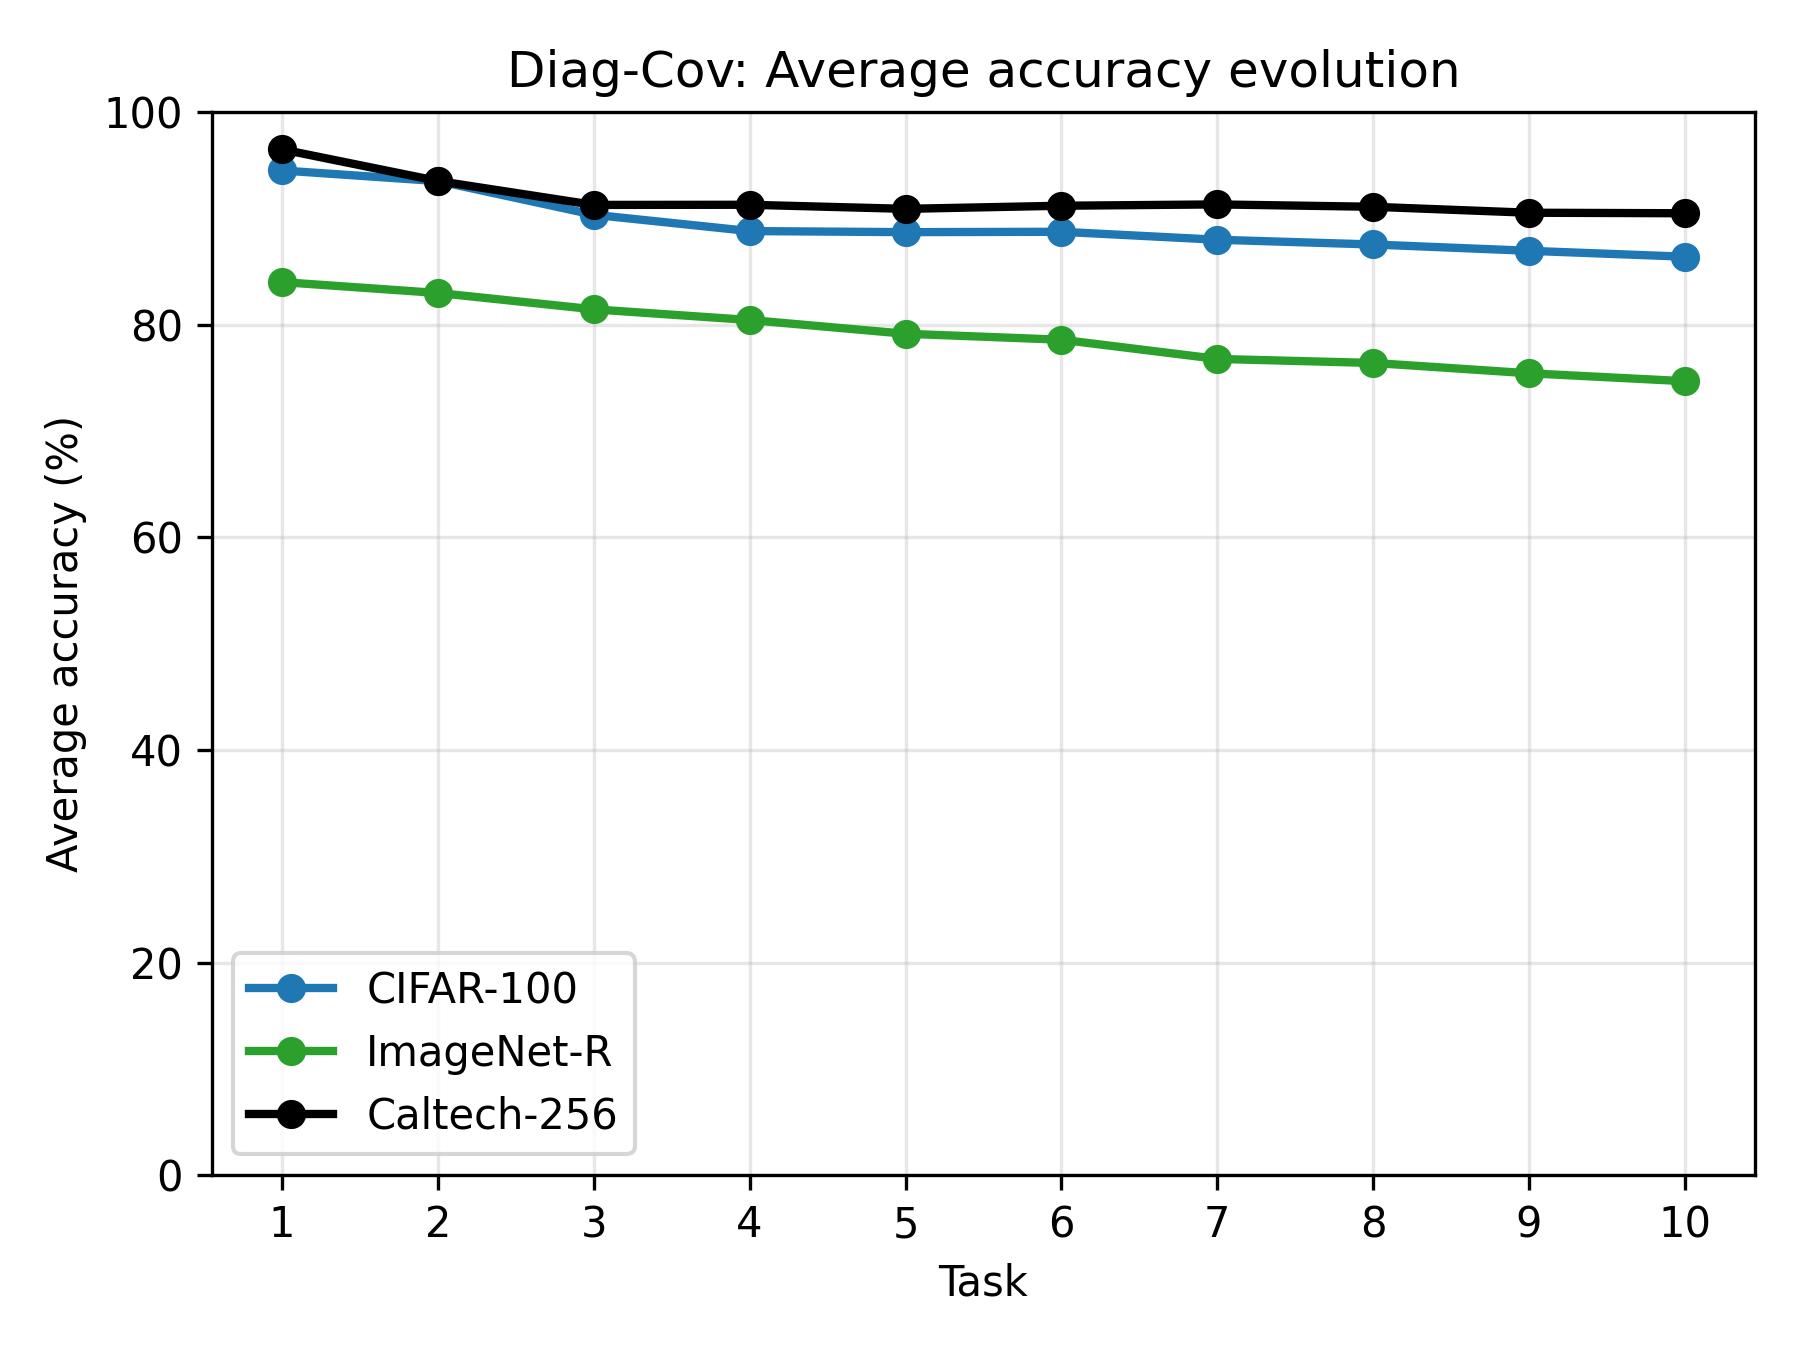
\includegraphics[width=0.32\linewidth]{imagenes/results/avg_accuracy_evolution_diagcov.png}}
	\hfill
	\subcaptionbox{Full-Cov}{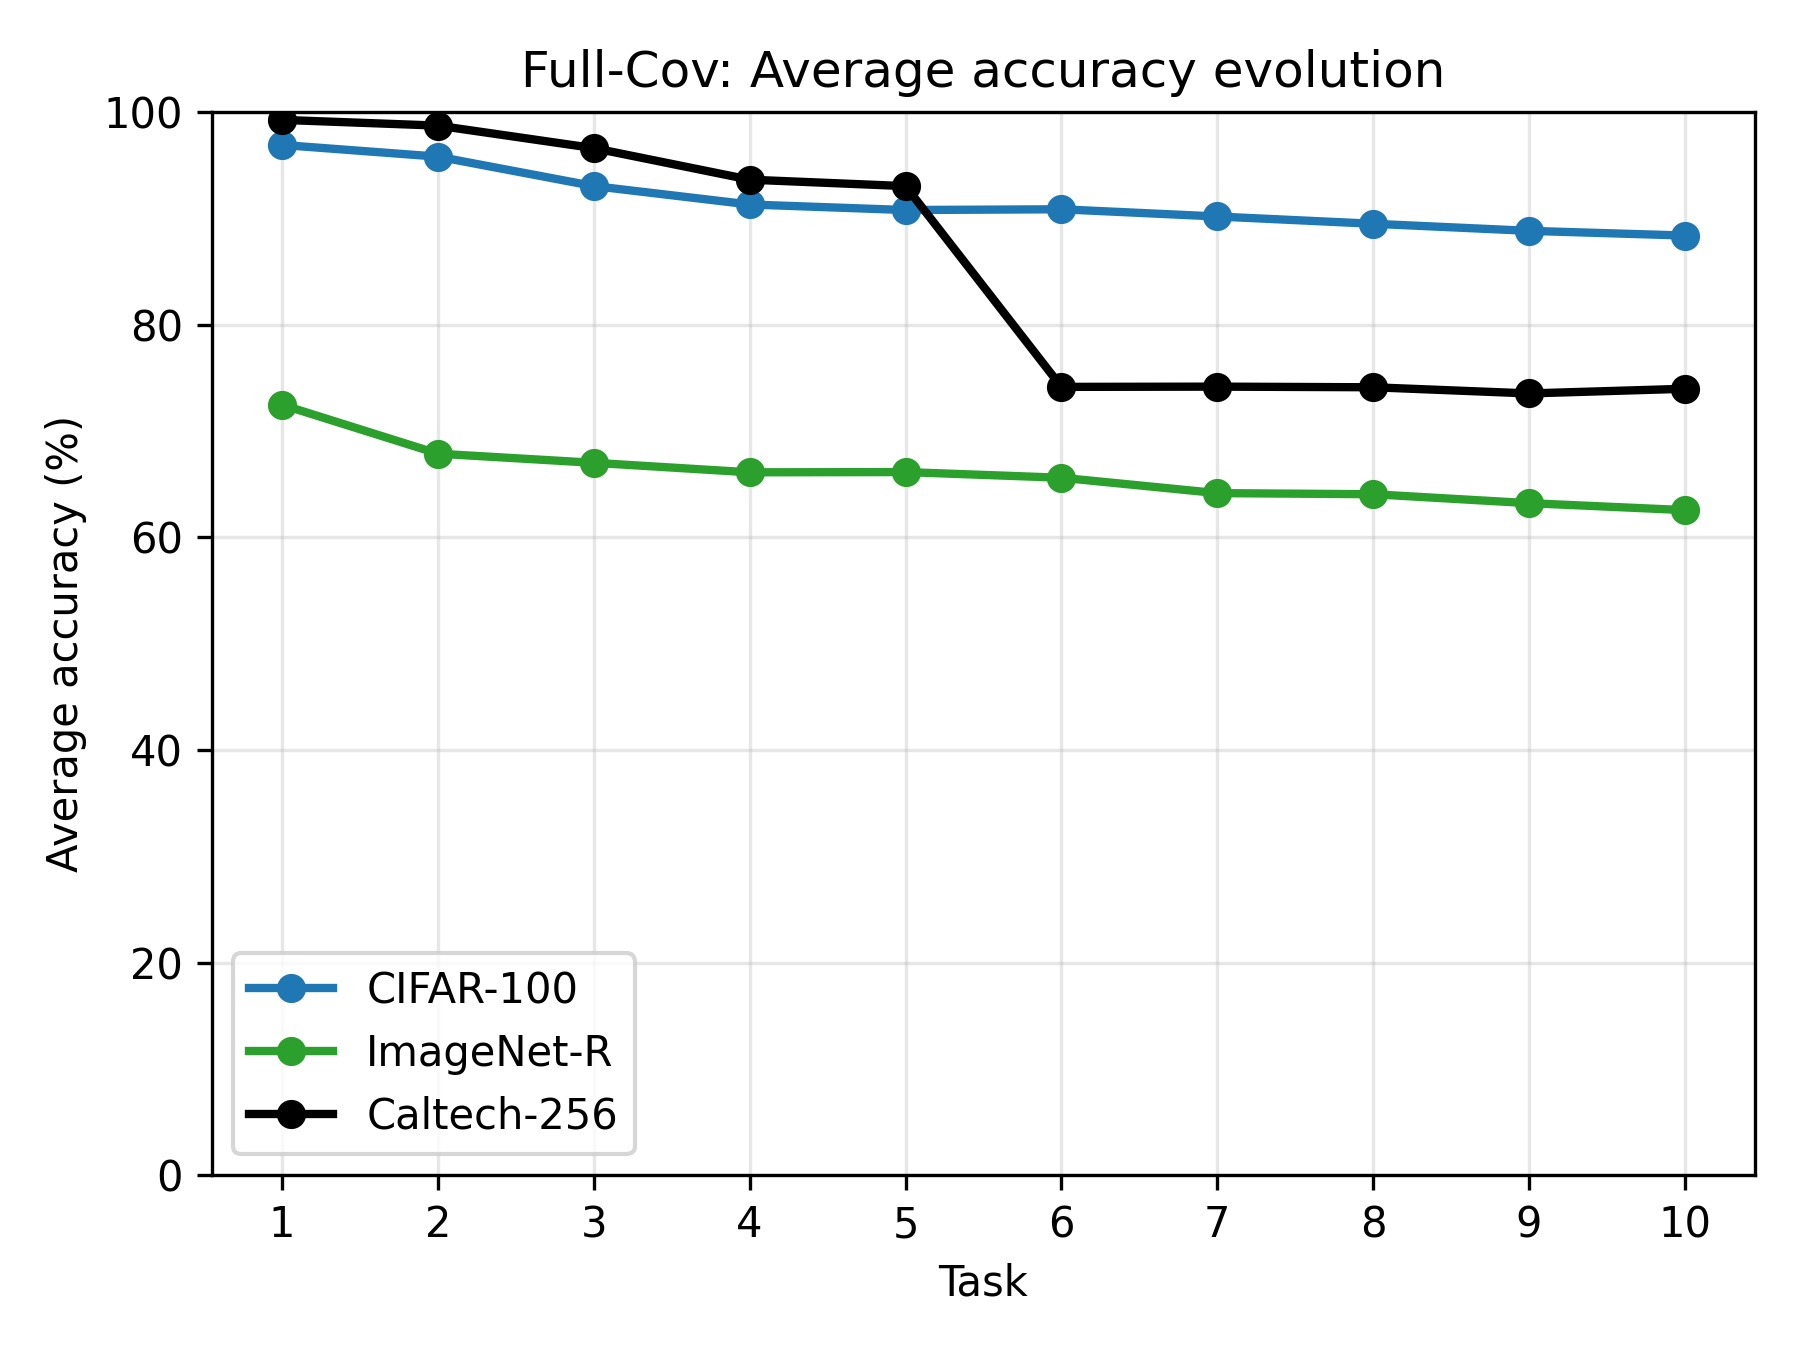
\includegraphics[width=0.32\linewidth]{imagenes/results/avg_accuracy_evolution_fullcov.png}}
	\hfill
	\subcaptionbox{MOG4-Shared}{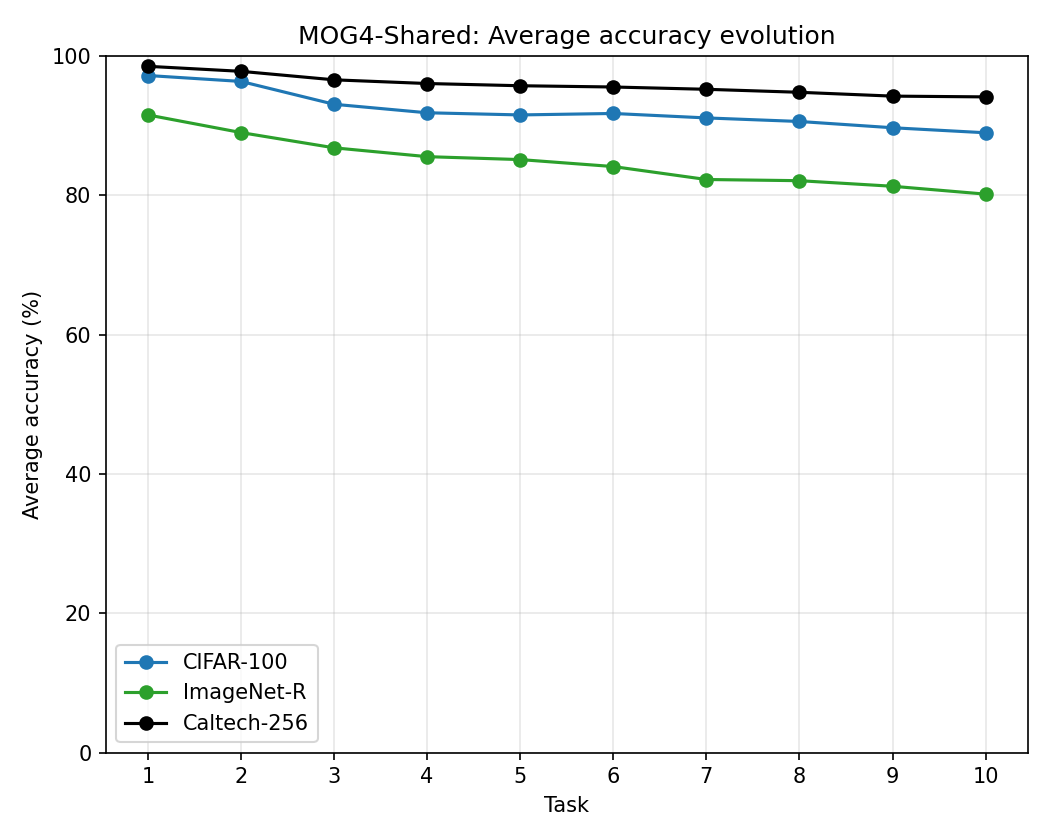
\includegraphics[width=0.32\linewidth]{imagenes/results/avg_accuracy_evolution_mog4shared.png}}
	\caption{Evolution of average accuracy across ten sequential tasks for CIFAR-100 (blue), ImageNet-R (green), and Caltech-256 (black), under (\textbf{a}) Diag-Cov, (\textbf{b}) Full-Cov, and (\textbf{c}) MOG4-Shared estimation.}
	\label{fig:avg_acc_evolution}
\end{figure}

This decline should not be read as forgetting in the usual sense. Every class-conditional Gaussian is estimated independently and frozen the moment its class is added, so no parameters from previously learned classes are ever overwritten: each class keeps, unchanged, the exact representation it was given when it was first learned. What grows with $t$ is not error on old classes caused by new ones, but the difficulty of the classification problem itself, since every extra task adds more competing prototypes for the Bayesian decision rule to tell apart. Figure~\ref{fig:bhattacharyya} quantifies this same mechanism through the decay of the minimum pairwise Bhattacharyya distance: as more classes are added, some pairs of prototypes inevitably move closer together in feature space, which raises the chance of confusion even though none of the individual class models has changed. The accuracy drop shown here is therefore a harder decision surface, not lost knowledge, and it matches the low forgetting values already reported in Table~\ref{tab:combined_benchmarks}. The next section develops this separability analysis in full.

\section{Inter-Class Separability}
\label{sec:interclass_results}

Before asking why some classes are harder than others, it helps to look at how accuracy is actually spread across classes once every one of them has been added to the stream. This section starts from that per-class picture, and then uses the geometry of the embedding space, through the Bhattacharyya and Euclidean distances between class prototypes, to explain why some classes end up harder to tell apart than others.

\subsection{Per-Class Accuracy Once All Classes Are Added}
\label{sec:an:recall_distributions}

Once every task has been added to the stream, the Diag-Cov classifier reaches overall accuracies of $86.6\%$, $90.2\%$, and $72.5\%$ on CIFAR-100, Caltech-256, and ImageNet-R respectively, while Full-Cov reaches $88.9\%$, $94.7\%$, and $74.7\%$ on those same benchmarks. Figures~\ref{fig:class_acc_hist_cifar}--\ref{fig:class_acc_hist_caltech} break these overall numbers down by class, showing how accuracy is actually spread across categories rather than being uniform.

\begin{figure}[htbp]
	\centering
	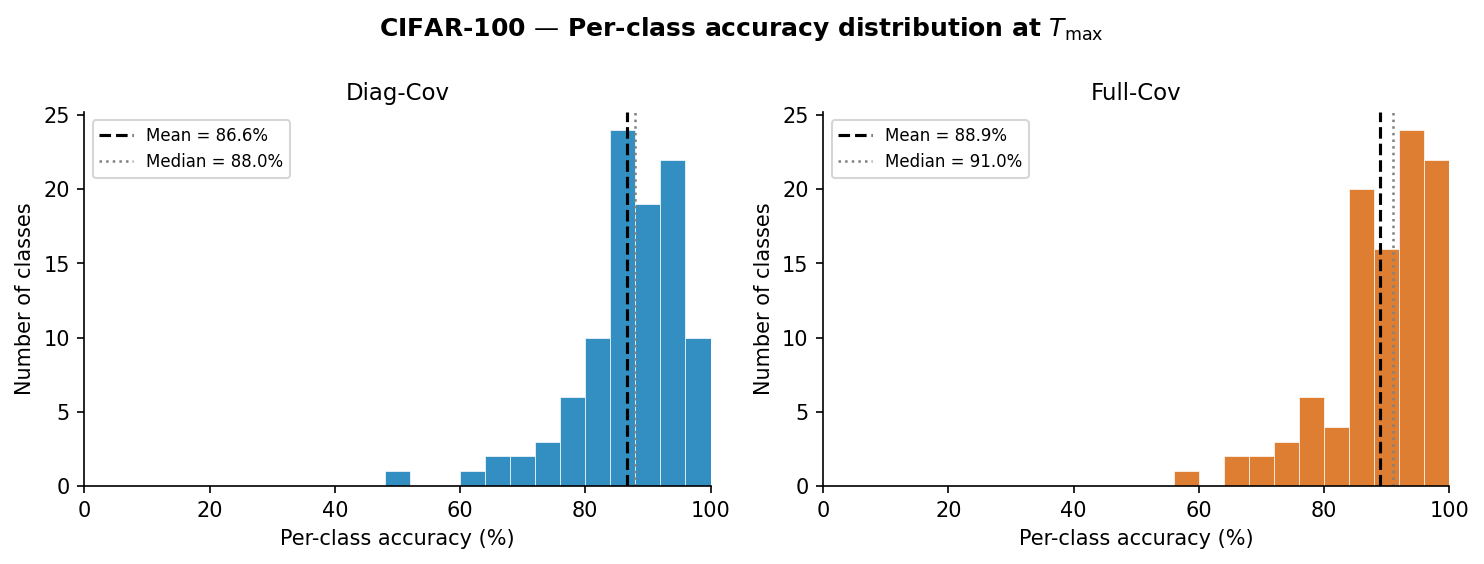
\includegraphics[width=0.99\linewidth]{imagenes/results/class_acc_hist_CIFAR100.png}
	\caption{Per-class accuracy once all classes have been added, for CIFAR-100 ($N=100$ classes). Left: Diag-Cov. Right: Full-Cov.}
	\label{fig:class_acc_hist_cifar}
\end{figure}

\begin{figure}[htbp]
	\centering
	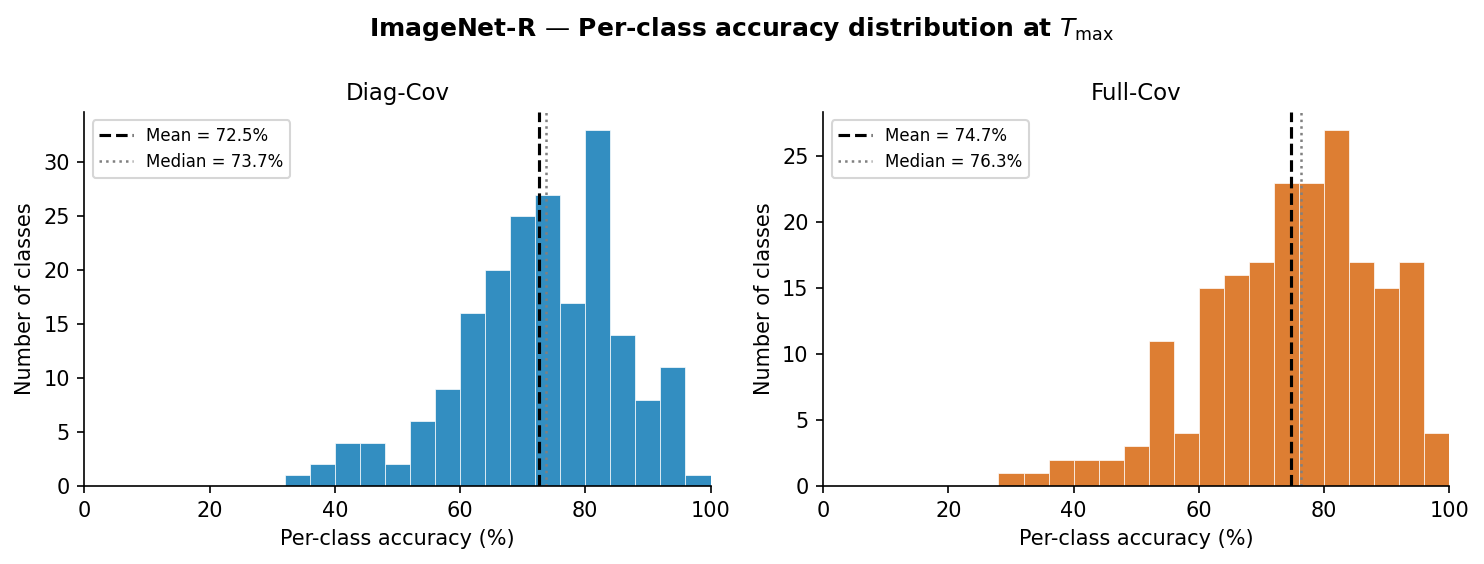
\includegraphics[width=0.99\linewidth]{imagenes/results/class_acc_hist_ImageNetR.png}
	\caption{Per-class accuracy once all classes have been added, for ImageNet-R ($N=200$ classes).}
	\label{fig:class_acc_hist_imagenetr}
\end{figure}

\begin{figure}[htbp]
	\centering
	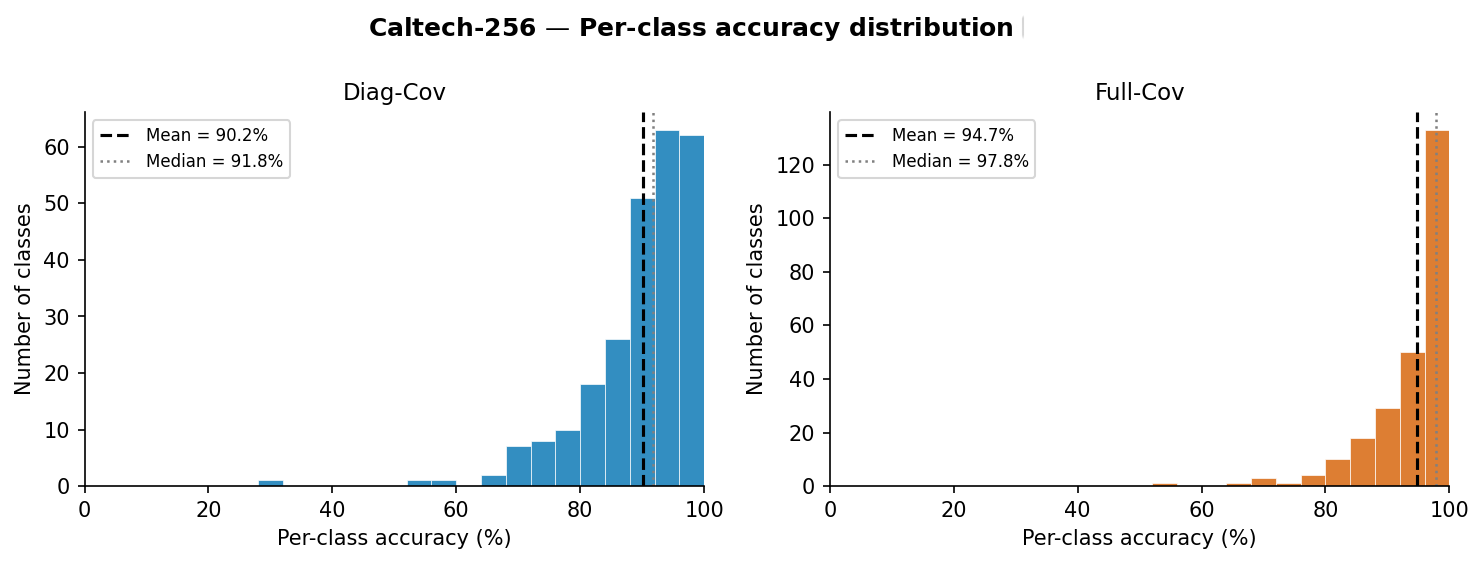
\includegraphics[width=0.99\linewidth]{imagenes/results/class_acc_hist_Caltech256.png}
	\caption{Per-class accuracy once all classes have been added, for Caltech-256 ($N=250$ classes).}
	\label{fig:class_acc_hist_caltech}
\end{figure}

The shapes of these histograms show two different pictures depending on the benchmark: on some, per-class accuracy is spread out across nearly the whole range, from very low to very high; on others, it stays tightly concentrated in one region. Either way, some classes always come out clearly better recognised than others.

On Split CIFAR-100, the recall profiles for both Diag-Cov and Full-Cov are tightly concentrated and broadly unimodal, skewed toward the highest accuracy bins. This concentration reflects the stable, well-behaved nature of low-resolution natural features, where most categories have compact feature distributions that single-component Gaussians approximate with little residual variance. Split Caltech-256 shows an even cleaner concentration peak; under Full-Cov estimation, the median shifts toward $97.8\%$, putting most of the dataset into a near-perfect recognition cluster. This shows that although high-resolution object photography introduces large variance across coordinates, its semantic categories occupy well isolated, linearly separable regions of the DINOv2 manifold, letting a full precision matrix separate the few remaining competitive boundaries.

Split ImageNet-R, by contrast, shows a dispersed, flat distribution with a long tail of low-accuracy classes extending down past the $40\%$ mark. Unlike the tight concentration seen in CIFAR-100 and Caltech-256, the visual features of ImageNet-R are not well concentrated. Because the imagery is intentionally out-of-distribution---spanning stylized art, cartoons, and hand-drawn sketches---the frozen foundation encoder maps these samples into broad, diffuse, and anisotropic representations. This lack of spatial concentration produces large intra-class variance and complex directional skewness, which limits the modeling capacity of single independent Gaussians.

As explained in Section~\ref{sec:incremental_update}, this gap between classes cannot come from forgetting in the usual sense: each class-conditional Gaussian is estimated once and frozen the moment its class is added, so nothing about how well an old class is modelled can change afterwards. If some classes still end up much harder than others once every task has been seen, the cause has to be something else, namely how close different classes actually sit to each other in the embedding space. The rest of this section looks at that directly.

\subsection{Class Overlap: Bhattacharyya and Euclidean Distances}
\label{sec:an:interclass}

To see how close different classes sit to each other in the embedding space, we use two complementary measures: the \emph{Bhattacharyya distance} $D_B$, which accounts for differences in both class means and covariances, and the plain \emph{Euclidean distance} $d_E = \|\boldsymbol{\mu}_i - \boldsymbol{\mu}_j\|_2$ between class mean vectors, which isolates mean separation alone.

\begin{figure}[htbp]
	\centering
	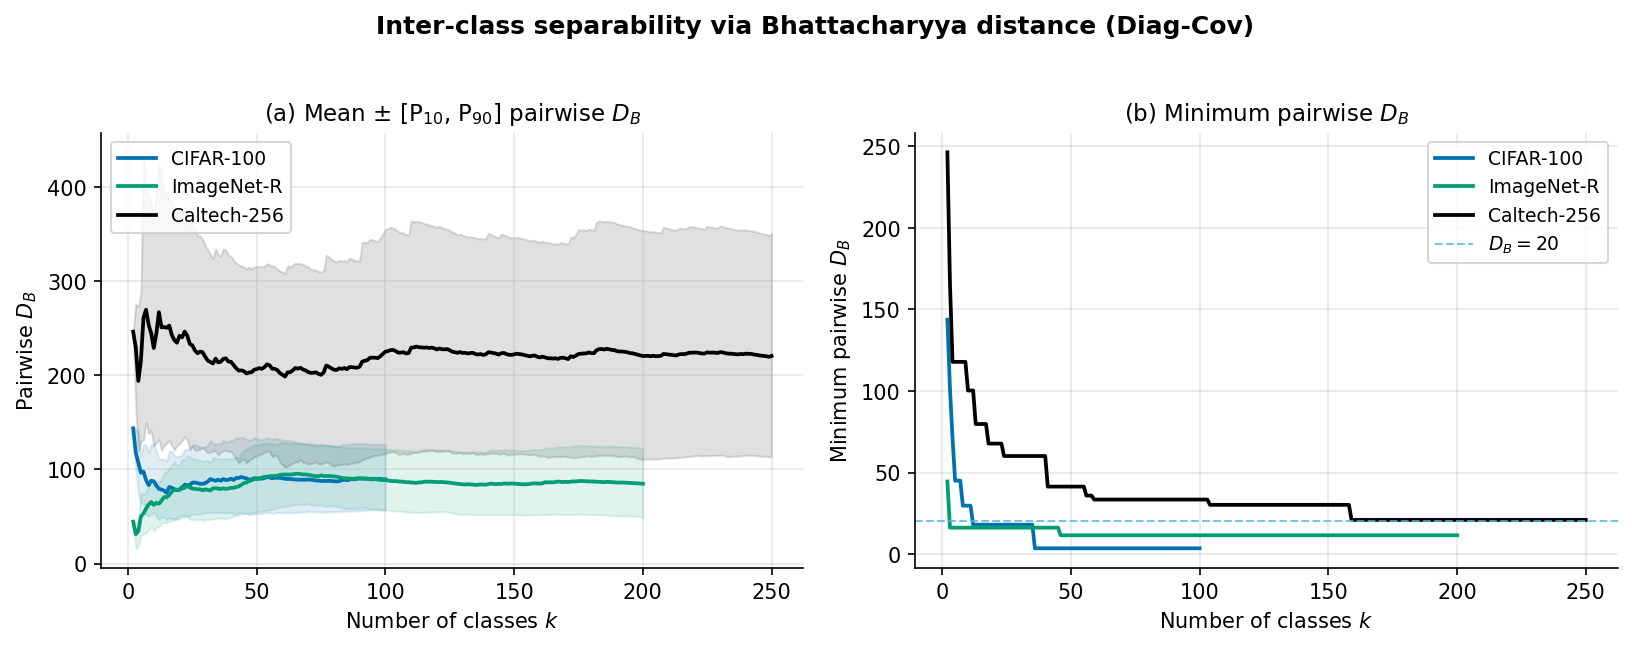
\includegraphics[width=0.99\linewidth]{imagenes/results/bhattacharyya_ab.png}
	\caption{%
		Inter-class separability under the Diag-Cov Gaussian model as the class
		set grows from $k=2$ to the full benchmark size.
		\textbf{(a)}~Mean pairwise $D_B$ with shaded $[\mathrm{P}_{10},\mathrm{P}_{90}]$ band.
		\textbf{(b)}~Minimum pairwise $D_B$; the dashed horizontal line marks $D_B\!=\!20$.%
	}
	\label{fig:bhattacharyya}
\end{figure}

\begin{figure}[htbp]
	\centering
	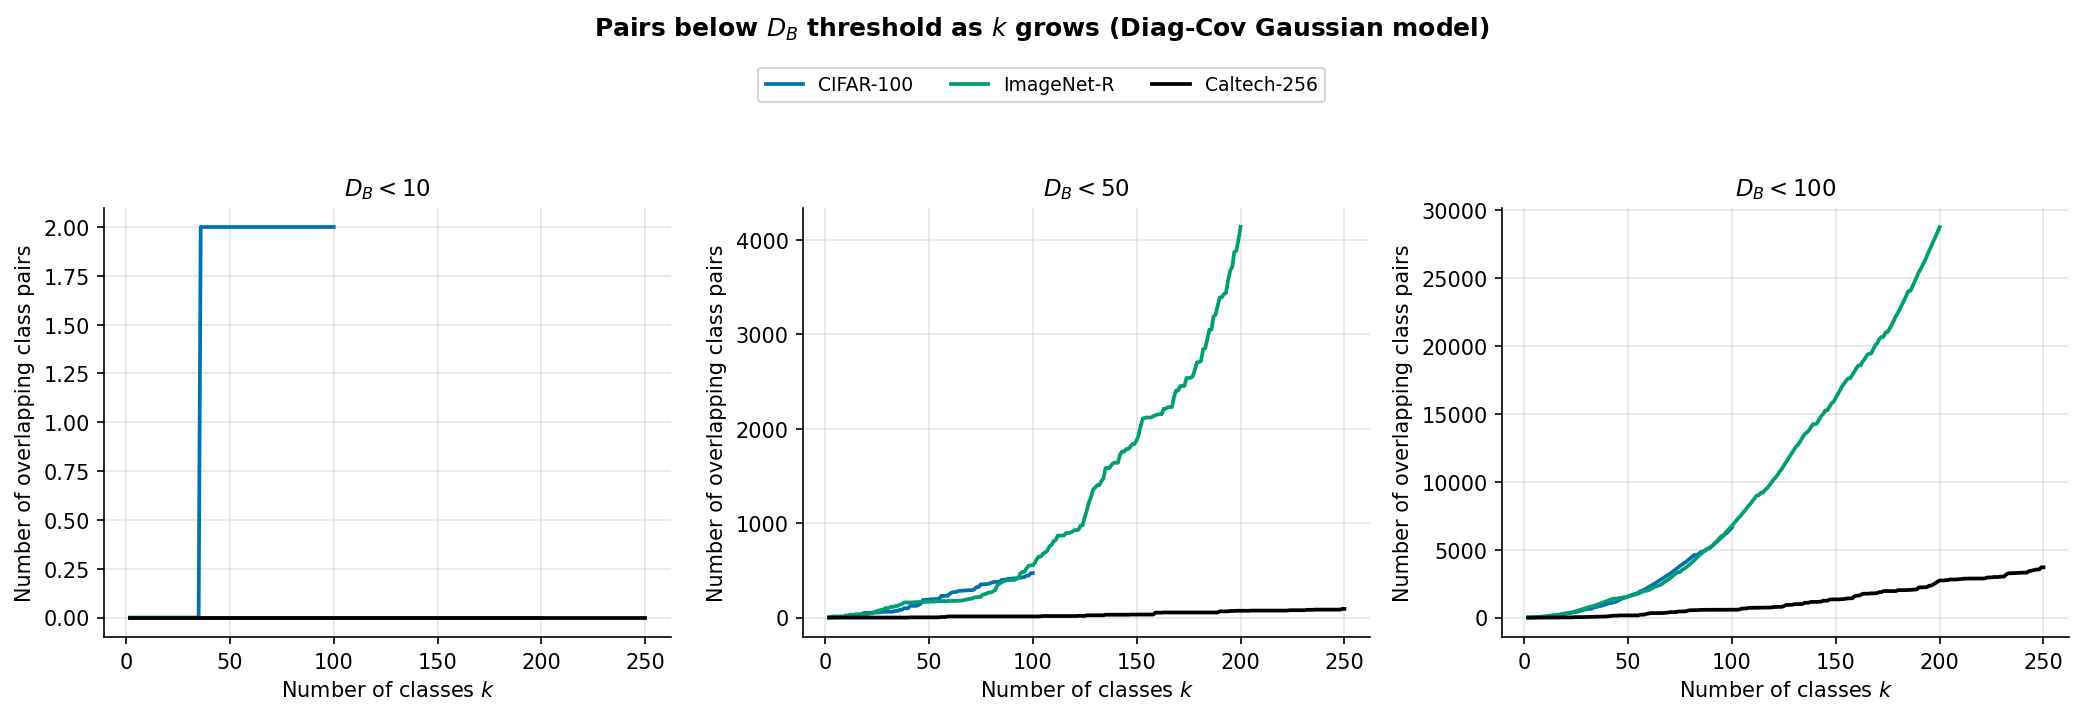
\includegraphics[width=0.99\linewidth]{imagenes/results/bhattacharyya_thresholds.png}
	\caption{%
		Count of class pairs below three overlap thresholds ($D_B < 10$, $D_B < 50$,
		$D_B < 100$) as the class set grows. Over $99.8\,\%$ of all pairs exceed
		$D_B\!=\!50$ on every benchmark.%
	}
	\label{fig:bhattacharyya_thresholds}
\end{figure}

\begin{figure}[htbp]
	\centering
	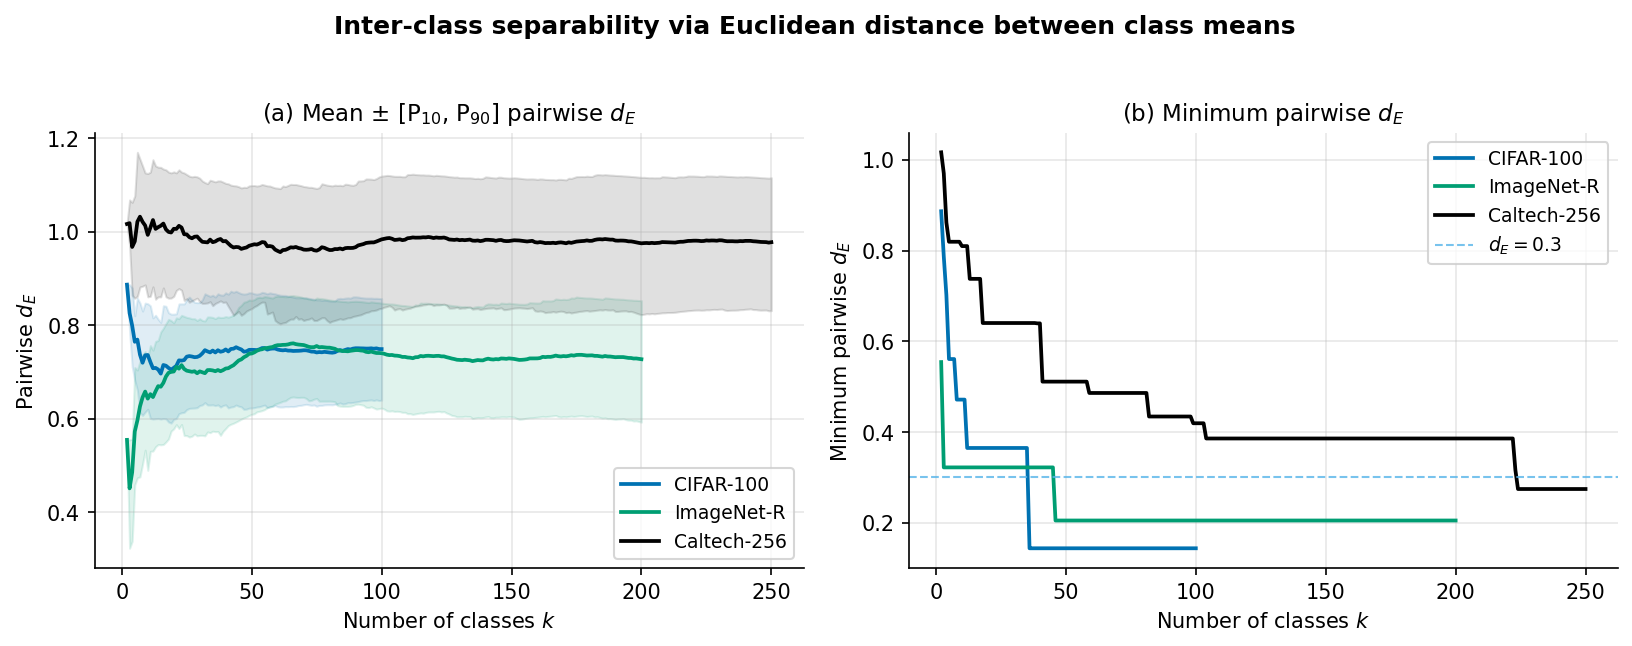
\includegraphics[width=0.99\linewidth]{imagenes/results/euclidean_ab.png}
	\caption{%
		Inter-class separability in terms of the plain Euclidean distance
		$d_E$ between class means, as the class set grows from $k=2$ to the
		full benchmark size.
		\textbf{(a)}~Mean pairwise $d_E$ with shaded $[\mathrm{P}_{10},\mathrm{P}_{90}]$ band.
		\textbf{(b)}~Minimum pairwise $d_E$.%
	}
	\label{fig:euclidean}
\end{figure}

\begin{figure}[htbp]
	\centering
	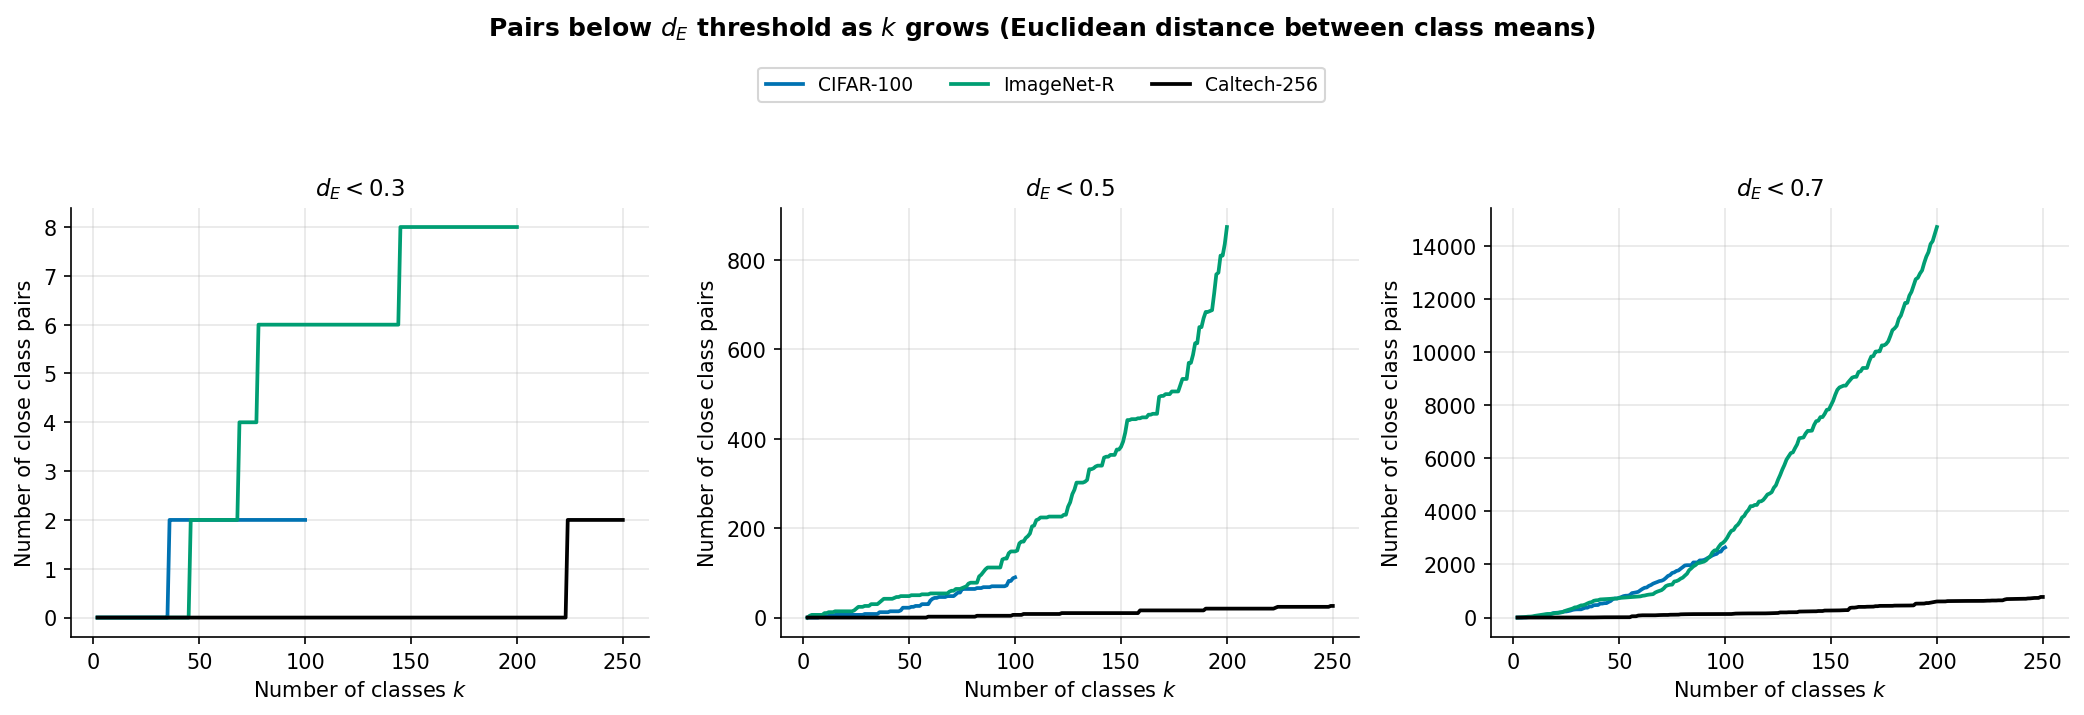
\includegraphics[width=0.99\linewidth]{imagenes/results/euclidean_thresholds.png}
	\caption{%
		Count of class pairs below three Euclidean-distance overlap thresholds
		as the class set grows, complementing the Bhattacharyya-based count of
		Figure~\ref{fig:bhattacharyya_thresholds}.%
	}
	\label{fig:euclidean_thresholds}
\end{figure}

The scaling trajectories of the pairwise Bhattacharyya distances (Figures~\ref{fig:bhattacharyya} and~\ref{fig:bhattacharyya_thresholds}) and mean Euclidean distances (Figures~\ref{fig:euclidean} and~\ref{fig:euclidean_thresholds}) show a consistent pattern across the foundation embedding manifolds. Rather than an overall compression of the representation space as tasks accumulate, the global layout of the features stays fairly stable, while performance is limited mainly by a small, heavy-tailed set of overlapping class pairs.

One sign of this stability is that both macro-averaged distance metrics plateau quickly across all benchmarks once around 30 categories are introduced. At full class-set size, the mean pairwise $D_B$ settles at $220.61$ for Caltech-256, $89.43$ for CIFAR-100, and $84.81$ for ImageNet-R. This same ordering is matched by the macro-averaged mean Euclidean distance, where Caltech-256 keeps a wide geometric separation of $\overline{d_E} = 0.978$, while CIFAR-100 and ImageNet-R stay more densely packed at $\overline{d_E} = 0.749$ and $\overline{d_E} = 0.727$, respectively. Caltech-256's clear separability advantage on both metrics reflects its greater visual and semantic diversity, which keeps per-class distributions distinct.

However, as the label space grows denser, the minimum pairwise distance metrics decay steadily, and this is the real driver behind the accuracy gaps between classes seen in the previous subsection. Once every class has been added, the minimum pairwise $D_B$ drops to $3.57$ on CIFAR-100, $11.54$ on ImageNet-R, and $20.96$ on Caltech-256. This localized crowding is confirmed by the Euclidean mean separation, which hits minimum values of $0.144$, $0.205$, and $0.275$ for the respective datasets.

Tracking the density thresholds shows that this crowding is an isolated effect rather than a general collapse of the space. Over $99.8\,\%$ of all possible class combinations stay well above a threshold of $D_B = 50$ on every evaluated benchmark. Similarly, class pairs with $d_E < 0.5$ make up only a small fraction of the total, accounting for $0.91\,\%$ of pairs in CIFAR-100, $2.20\,\%$ in ImageNet-R, and just $0.04\,\%$ in Caltech-256.

So the classifier is not working in a uniformly collapsed or muddy feature space. Instead, the accuracy ceilings ($88.87\%$ for CIFAR-100, $77.99\%$ for ImageNet-R, and $94.36\%$ for Caltech-256 under the strongest Gaussian configurations) are set by a small number of highly confusable prototype pairs, which is exactly what produces the long low-accuracy tail seen on ImageNet-R in the previous subsection.

The two metrics act as complementary diagnostics for these failure points. While $d_E$ isolates pure first-order geometric separation between prototype centroids, $D_B$ also penalizes covariance shape and volume differences. This explains why a pair such as \textit{boy}/\textit{girl} in CIFAR-100 stands out as the single biggest source of confusion in the system: it combines a very small geometric centroid distance ($d_E = 0.145$) with nearly identical, overlapping second-order covariance structures, pushing the probabilistic separation down to its minimum. To see exactly which classes this affects and why, we now look at individual class confusion patterns, examining the visual and geometric identities of the worst-performing classes in the system.

\subsection{Worst-Performing Classes and Failure Diagnostics}
\label{sec:worst_classes}

Breaking macro-level performance metrics down into class-specific failure points gives a clearer view of the resolution limits of the visual foundation embedding space and the boundaries of each covariance parameterisation. To isolate these failure cases, we rank and track the five object categories with the lowest per-class recall scores across all benchmarks.

We analyze these failure patterns across two parameterisations: Table~\ref{tab:worst_diag} characterizes the five lowest-performing classes under the independent feature assumptions of the Diagonal Covariance model, while Table~\ref{tab:worst_full} evaluates the corresponding distribution shifts and re-orderings under the regularized Full Covariance parameterisation. For both, the table records the empirical recall, the dominant confusion sink, the localized pairwise Bhattacharyya distance ($D_B$), and the Euclidean distance ($d_E$) to that primary target. These are compared directly against the dataset-level macro-averaged distances ($\overline{D_B}$ and $\overline{d_E}$) established in Section~\ref{sec:an:interclass}. Localized metrics falling well below these macro-averages give a direct geometric indication of significant prototype overlap.

\begin{table}[htbp]
	\centering
	\small
	\caption{Analysis of the five lowest-recall classes on each benchmark under Diagonal Covariance (Diag-Cov). $\text{Conf.}\%$ represents the percentage of errors directed toward the main confusion target. $D_B$ and $d_E$ denote the pairwise Bhattacharyya and Euclidean distances to the main confusion target, respectively, while $\overline{D_B}$ and $\overline{d_E}$ represent the macro-averaged pairwise distances across the entire dataset split.}
	\label{tab:worst_diag}
	\begin{adjustbox}{width=0.95\columnwidth, center}
		\small
		\begin{tabular}{llccccccc}
			\toprule
			\textbf{Dataset} & \textbf{Class} & \textbf{Acc\%} & \textbf{Main Confusion} & \textbf{Conf.\%} & $D_B$ & $\overline{D_B}$ & $d_E$ & $\overline{d_E}$ \\
			\midrule
			\textbf{Split CIFAR-100}
			& \textit{boy}          & 50.0 & \textit{girl}       & 30.0 &   3.45 & 89.43 & 0.145 & 0.749 \\
			& \textit{maple\_tree} & 60.0 & \textit{oak\_tree}  & 19.0 & 19.41 & 89.43 & 0.327 & 0.749 \\
			& \textit{girl}         & 65.0 & \textit{boy}        & 23.0 &   3.45 & 89.43 & 0.145 & 0.749 \\
			& \textit{cloud}        & 65.0 & \textit{sea}        &  8.0 & 30.54 & 89.43 & 0.451 & 0.749 \\
			& \textit{shrew}        & 69.0 & \textit{mouse}      & 16.0 & 16.45 & 89.43 & 0.331 & 0.749 \\
			\midrule
			\textbf{Split ImageNet-R}
			& \textit{cabbage}        & 35.3 & \textit{vase}           & 17.6 & 50.50 & 84.81 & 0.587 & 0.727 \\
			& \textit{saint\_bernard} & 36.4 & \textit{basset\_hound}  &  9.1 & 66.44 & 84.81 & 0.643 & 0.727 \\
			& \textit{bow\_tie}       & 39.3 & \textit{scarf}          & 21.4 & 16.57 & 84.81 & 0.331 & 0.727 \\
			& \textit{beaver}         & 40.0 & \textit{backpack}       &  8.6 & 34.74 & 84.81 & 0.500 & 0.727 \\
			& \textit{bee}            & 41.6 & \textit{fly}            & 15.6 & 20.51 & 84.81 & 0.378 & 0.727 \\
			\midrule
			\textbf{Split Caltech-256}
			& \textit{top-hat}        & 31.2 & \textit{cowboy-hat}     & 31.2 & 29.75 & 220.61 & 0.319 & 0.978 \\
			& \textit{paperclip}      & 52.6 & \textit{drinking-straw} & 21.1 & 62.94 & 220.61 & 0.645 & 0.978 \\
			& \textit{canoe}          & 57.1 & \textit{people}         & 28.6 & 57.87 & 220.61 & 0.641 & 0.978 \\
			& \textit{drinking-straw} & 64.7 & \textit{people}         & 11.8 & 27.33 & 220.61 & 0.465 & 0.978 \\
			& \textit{traffic-light}  & 65.0 & \textit{people}         & 15.0 & 66.27 & 220.61 & 0.675 & 0.978 \\
			\bottomrule
		\end{tabular}
	\end{adjustbox}
\end{table}

Table~\ref{tab:worst_full} details the equivalent classification landscapes under the regularized Full Covariance model. While the low-recall sets overlap heavily on the localized natural structures of Split CIFAR-100, they diverge substantially on the high-resolution object coordinates of Split Caltech-256. Because $\overline{D_B}$ and $\overline{d_E}$ represent fundamental global properties of the static underlying feature distributions, they remain identical to the baseline values reported in Table~\ref{tab:worst_diag}. 

\begin{table}[htbp]
	\centering
	\small
	\caption{Analysis of the five lowest-recall classes on each benchmark under Full Covariance (Full-Cov). Columns match the structure of Table~\ref{tab:worst_diag}; the probabilistic distance $D_B$ is computed using the regularized diagonal components for numeric consistency across the imbalanced stream.}
	\label{tab:worst_full}
	\begin{adjustbox}{width=0.95\columnwidth, center}
		\small
		\begin{tabular}{llccccccc}
			\toprule
			\textbf{Dataset} & \textbf{Class} & \textbf{Acc\%} & \textbf{Main Confusion} & \textbf{Conf.\%} & $D_B$ & $\overline{D_B}$ & $d_E$ & $\overline{d_E}$ \\
			\midrule
			\textbf{Split CIFAR-100}
			& \textit{boy}          & 58.0 & \textit{girl}       & 16.0 &   3.45 & 89.43 & 0.145 & 0.749 \\
			& \textit{girl}         & 67.0 & \textit{boy}        & 15.0 &   3.45 & 89.43 & 0.145 & 0.749 \\
			& \textit{otter}        & 67.0 & \textit{seal}       &  8.0 & 16.42 & 89.43 & 0.342 & 0.749 \\
			& \textit{maple\_tree} & 68.0 & \textit{oak\_tree}  & 19.0 & 19.41 & 89.43 & 0.327 & 0.749 \\
			& \textit{forest}       & 68.0 & \textit{pine\_tree} &  7.0 & 25.46 & 89.43 & 0.422 & 0.749 \\
			\midrule
			\textbf{Split ImageNet-R}
			& \textit{bow\_tie}    & 28.6 & \textit{cowboy\_hat} & 14.3 & 14.51 & 84.81 & 0.323 & 0.727 \\
			& \textit{bee}          & 33.8 & \textit{fly}        & 11.7 & 20.51 & 84.81 & 0.378 & 0.727 \\
			& \textit{beaver}       & 37.1 & \textit{backpack}   &  8.6 & 34.74 & 84.81 & 0.500 & 0.727 \\
			& \textit{cowboy\_hat} & 39.0 & \textit{hammer}     &  6.8 & 21.01 & 84.81 & 0.404 & 0.727 \\
			& \textit{candle}       & 40.7 & \textit{stole}      &  9.3 & 19.73 & 84.81 & 0.379 & 0.727 \\
			\midrule
			\textbf{Split Caltech-256}
			& \textit{drinking-straw}  & 52.9 & \textit{soda-can}     & 11.8 &  51.11 & 220.61 & 0.614 & 0.978 \\
			& \textit{people}          & 66.7 & \textit{picnic-table} &  4.8 &  55.38 & 220.61 & 0.619 & 0.978 \\
			& \textit{top-hat}          & 68.8 & \textit{wine-bottle}  &  6.2 & 100.90 & 220.61 & 0.802 & 0.978 \\
			& \textit{american-flag}   & 70.0 & \textit{speed-boat}   &  5.0 & 108.32 & 220.61 & 0.823 & 0.978 \\
			& \textit{bowling-ball}    & 71.4 & \textit{bowling-pin}  & 14.3 &  68.73 & 220.61 & 0.644 & 0.978 \\
			\bottomrule
		\end{tabular}
	\end{adjustbox}
\end{table}

To ground these proximity numbers in something visual, we look at typical images taken directly from the benchmark data streams. Figures~\ref{fig:worst_repr_cifar}, \ref{fig:worst_repr_imagenetr}, and~\ref{fig:worst_repr_caltech} present the target classes side by side with their main cross-category confusion partners, the samples most frequently confused by the classifier. Looking at these cross-class pairs shows the structural and semantic similarities that drive the lower tails of our recall curves.

% ==========================================
% FIGURE 1: CIFAR-100 (4x2 Grid) - FIXED
% ==========================================
\begin{figure}[htbp]
	\centering
	
	% --- Row 1 ---
	\begin{minipage}[t]{0.23\linewidth}
		\centering
		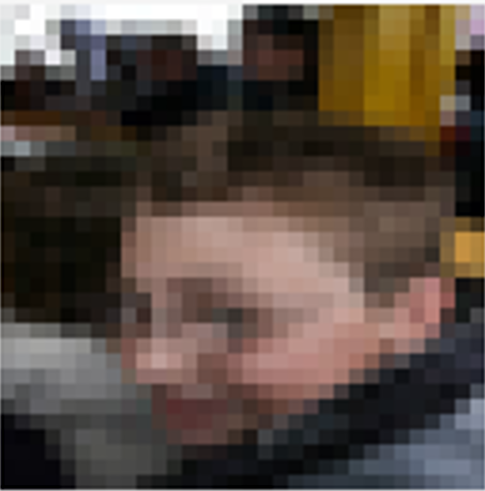
\includegraphics[width=0.99\linewidth]{imagenes/results/cifar_100/boy.png}\\
		{\small (a) Boy}
	\end{minipage}\hfill
	\begin{minipage}[t]{0.23\linewidth}
		\centering
		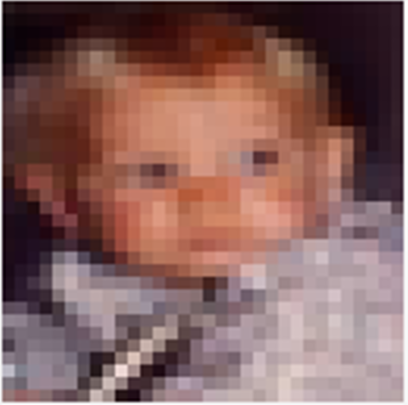
\includegraphics[width=0.99\linewidth]{imagenes/results/cifar_100/girl.png}\\
		{\small (b) Girl}
	\end{minipage}\hfill
	\begin{minipage}[t]{0.23\linewidth}
		\centering
		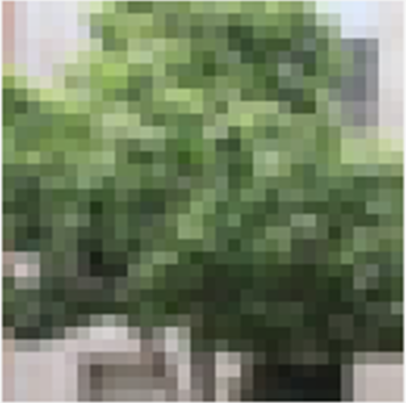
\includegraphics[width=0.99\linewidth]{imagenes/results/cifar_100/oak_tree.png}\\
		{\small (c) Oak Tree}
	\end{minipage}\hfill
	\begin{minipage}[t]{0.23\linewidth}
		\centering
		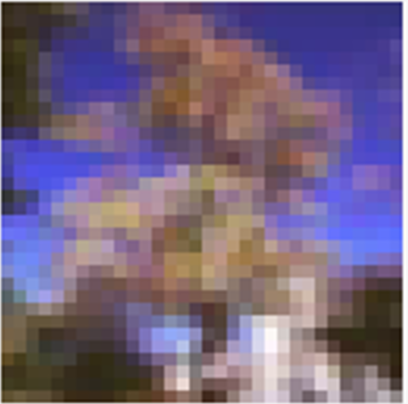
\includegraphics[width=0.99\linewidth]{imagenes/results/cifar_100/maple_tree.png}\\
		{\small (d) Maple Tree}
	\end{minipage}
	
	\vspace{0.4cm}
	
	% --- Row 2 ---
	\begin{minipage}[t]{0.23\linewidth}
		\centering
		
\includegraphics[width=0.99\linewidth]{imagenes/results/cifar_100/cloud.png}\\
		{\small (e) Cloud}
	\end{minipage}\hfill
	\begin{minipage}[t]{0.23\linewidth}
		\centering
		
\includegraphics[width=0.99\linewidth]{imagenes/results/cifar_100/sea.png}\\
		{\small (f) Sea}
	\end{minipage}\hfill
	\begin{minipage}[t]{0.23\linewidth}
		\centering
		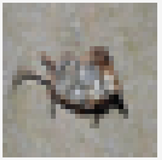
\includegraphics[width=0.99\linewidth]{imagenes/results/cifar_100/shrew.png}\\
		{\small (g) Shrew}
	\end{minipage}\hfill
	\begin{minipage}[t]{0.23\linewidth}
		\centering
		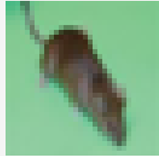
\includegraphics[width=0.99\linewidth]{imagenes/results/cifar_100/mouse.png}\\
		{\small (h) Mouse}
	\end{minipage}
	
	\caption{Representative visual specimens of the primary low-recall classes and corresponding confusion sinks on the Split CIFAR-100 benchmark, mapped to the tracking trends outlined in Table~\ref{tab:worst_diag} and Table~\ref{tab:worst_full}.}
	\label{fig:worst_repr_cifar}
\end{figure}

% ==========================================
% FIGURE 2: ImageNet-R (5x2 Grid)
% ==========================================
\begin{figure}[htbp]
	\centering
	
	% --- Row 1: First 5 images ---
	\begin{minipage}[t]{0.18\linewidth}
		\centering
		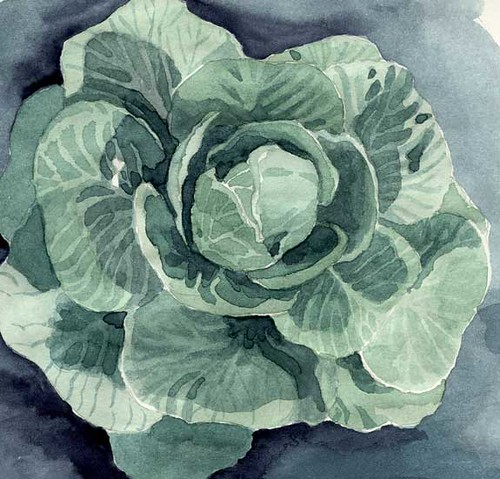
\includegraphics[width=0.9\linewidth]{imagenes/results/imagenetr/cabbage.jpg}\\
		{\small (a) Cabbage}
	\end{minipage}\hfill
	\begin{minipage}[t]{0.18\linewidth}
		\centering
		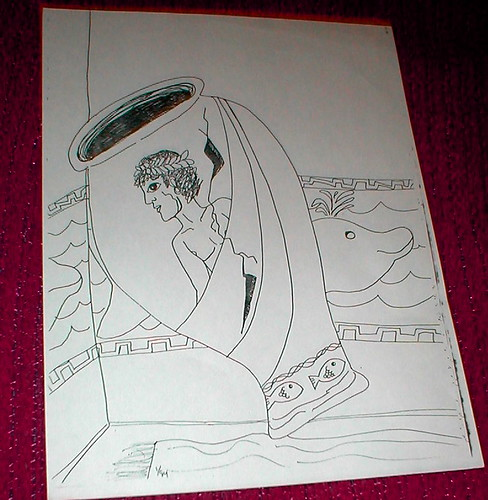
\includegraphics[width=0.9\linewidth]{imagenes/results/imagenetr/vase.jpg}\\
		{\small (b) Vase}
	\end{minipage}\hfill
	\begin{minipage}[t]{0.18\linewidth}
		\centering
		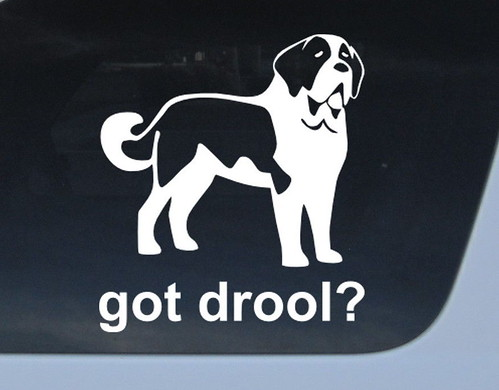
\includegraphics[width=0.9\linewidth]{imagenes/results/imagenetr/saint_bernard.jpg}\\
		{\small (c) Saint Bernard}
	\end{minipage}\hfill
	\begin{minipage}[t]{0.18\linewidth}
		\centering
		
\includegraphics[width=0.9\linewidth]{imagenes/results/imagenetr/basset_hound.jpg}\\
		{\small (d) Basset Hound}
	\end{minipage}\hfill
	\begin{minipage}[t]{0.18\linewidth}
		\centering
		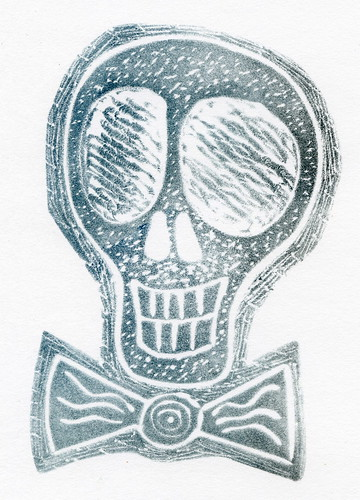
\includegraphics[width=0.9\linewidth]{imagenes/results/imagenetr/bow_tie.jpg}\\
		{\small (e) Bow Tie}
	\end{minipage}
	
	\vspace{0.4cm}
	
	% --- Row 2: Remaining 5 images ---
	\begin{minipage}[t]{0.18\linewidth}
		\centering
		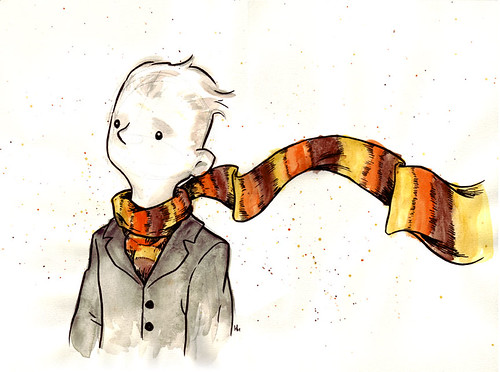
\includegraphics[width=0.9\linewidth]{imagenes/results/imagenetr/scarf.jpg}\\
		{\small (f) Scarf}
	\end{minipage}\hfill
	\begin{minipage}[t]{0.18\linewidth}
		\centering
		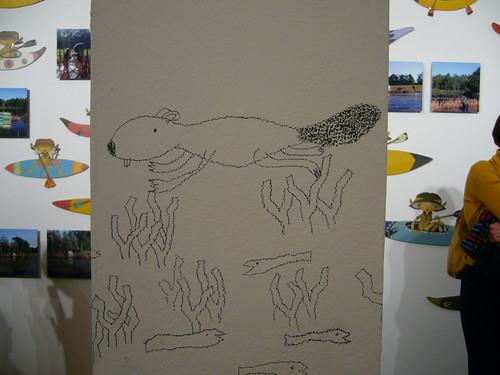
\includegraphics[width=0.9\linewidth]{imagenes/results/imagenetr/beaver.jpg}\\
		{\small (g) Beaver}
	\end{minipage}\hfill
	\begin{minipage}[t]{0.18\linewidth}
		\centering
		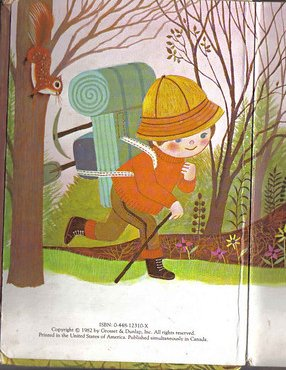
\includegraphics[width=0.9\linewidth]{imagenes/results/imagenetr/backpack.jpg}\\
		{\small (h) Backpack}
	\end{minipage}\hfill
	\begin{minipage}[t]{0.18\linewidth}
		\centering
		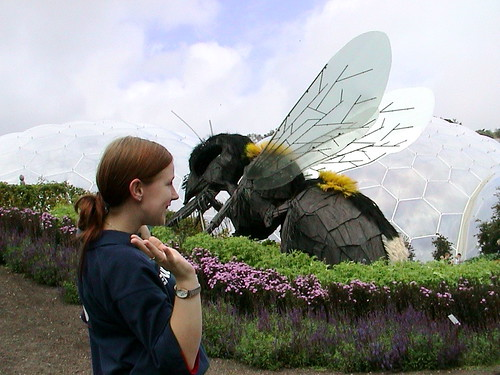
\includegraphics[width=0.9\linewidth]{imagenes/results/imagenetr/bee.jpg}\\
		{\small (i) Bee}
	\end{minipage}\hfill
	\begin{minipage}[t]{0.18\linewidth}
		\centering
		
\includegraphics[width=0.9\linewidth]{imagenes/results/imagenetr/fly.jpg}\\
		{\small (j) Fly}
	\end{minipage}
	
	\caption{Representative specimens from Split ImageNet-R mapped to the tracking trends outlined in Table~\ref{tab:worst_diag} and Table~\ref{tab:worst_full}, showing the non-photographic style of the dataset.}
	\label{fig:worst_repr_imagenetr}
\end{figure}

% ==========================================
% FIGURE 3: Caltech-256 (4 + 3 Centered Grid)
% ==========================================
\begin{figure}[htbp]
	\centering
	
	% --- Row 1 (4 items) ---
	\begin{minipage}[t]{0.23\linewidth}
		\centering
		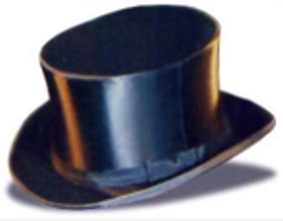
\includegraphics[width=0.8\linewidth]{imagenes/results/caltech/top_hat.png}\\
		{\small (a) Top Hat}
	\end{minipage}\hfill
	\begin{minipage}[t]{0.23\linewidth}
		\centering
		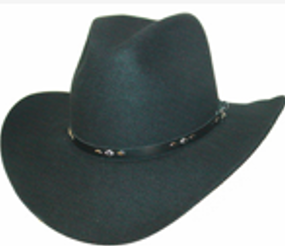
\includegraphics[width=0.8\linewidth]{imagenes/results/caltech/cowboy_hat.png}\\
		{\small (b) Cowboy Hat}
	\end{minipage}\hfill
	\begin{minipage}[t]{0.23\linewidth}
		\centering
		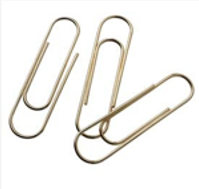
\includegraphics[width=0.8\linewidth]{imagenes/results/caltech/paperclip.png}\\
		{\small (c) Paperclip}
	\end{minipage}\hfill
	\begin{minipage}[t]{0.23\linewidth}
		\centering
		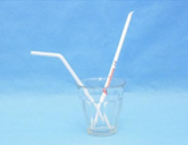
\includegraphics[width=0.8\linewidth]{imagenes/results/caltech/drinking_straw.png}\\
		{\small (d) Drinking Straw}
	\end{minipage}
	
	\vspace{0.4cm}
	
	% --- Row 2 (3 items balanced in the center) ---
	\hfill
	\begin{minipage}[t]{0.23\linewidth}
		\centering
		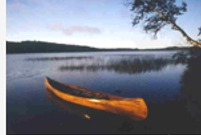
\includegraphics[width=0.8\linewidth]{imagenes/results/caltech/cannoe.png}\\
		{\small (e) Canoe}
	\end{minipage}\hfill
	\begin{minipage}[t]{0.23\linewidth}
		\centering
		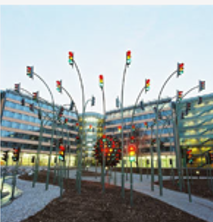
\includegraphics[width=0.8\linewidth]{imagenes/results/caltech/traffic_light.png}\\
		{\small (f) Traffic Light}
	\end{minipage}\hfill
	\begin{minipage}[t]{0.23\linewidth}
		\centering
		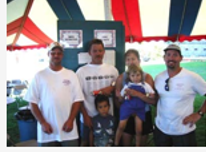
\includegraphics[width=0.8\linewidth]{imagenes/results/caltech/people.png}\\
		{\small (g) People}
	\end{minipage}\hfill\null
	
	\caption{Representative visual entities comprising the minimum separability boundary on the Split Caltech-256 stream mapped to the tracking trends outlined in Table~\ref{tab:worst_diag} and Table~\ref{tab:worst_full}.}
	\label{fig:worst_repr_caltech}
\end{figure}

This qualitative visual inspection confirms the reasoning behind the statistical proximity metrics recorded in our diagnostic tables. Categories such as \textit{boy} and \textit{girl} (Figure~\ref{fig:worst_repr_cifar}a--b), captured at the limited $32\times32$ pixel resolution of Split CIFAR-100, share nearly identical facial structures, skin tone distributions, and foreground composition. Similarly, the overlap between \textit{cloud} and \textit{sea} (Figure~\ref{fig:worst_repr_cifar}e--f) is driven by very similar global color palettes and low-frequency texture statistics, where the boundary between a cloudy sky and an ocean horizon becomes visually continuous. Given these strong semantic and stylistic similarities, it is expected from a generative perspective that their respective class-conditional feature distributions end up in near-coincident regions of the embedding space. The resulting cross-class confusion is therefore not caused by parameter degradation or catastrophic forgetting, but is a natural consequence of modeling independent probability densities over visual representations that are genuinely ambiguous.

\subsection{Synthesis of Inter-Class Confusion and Structural Bounds}
\label{sec:an:confusion}

The pairwise relationships extracted from the distributions once every class has been added (Tables~\ref{tab:worst_diag} and~\ref{tab:worst_full}) give a localized explanation for the separability trends seen across the benchmarks. The framework itself is not breaking down; the residual classification error concentrates in a small tail of highly confusable class pairs, and that tail is what shows where the representation's semantic boundaries actually sit.

This localized failure breaks down into three patterns:
\begin{itemize}
	\item \textbf{Semantic and Visual Near-Synonyms:} The most notable confusion comes from pairs that share basic silhouette, texture, or composition under DINOv2's representation. Cases such as \textit{boy}$\leftrightarrow$\textit{girl} ($D_B = 3.45$, $d_E = 0.145$), \textit{bow\_tie}$\leftrightarrow$\textit{scarf} ($D_B = 16.57$), and \textit{top-hat}$\leftrightarrow$\textit{cowboy-hat} ($D_B = 29.75$) show co-located distributions, where high-frequency discriminative features are largely absent from frozen, general-purpose embeddings.
	\item \textbf{Contextual and Manifold Sinks:} Proximity in the embedding space often comes from shared background or composition rather than category membership. This is shown by the overlap of \textit{cloud}$\leftrightarrow$\textit{sea} ($D_B = 30.54$) through matching color palettes, and by broad categories like \textit{people} acting as confusion sinks for unrelated objects (\textit{canoe}, \textit{drinking-straw}) that happen to be photographed with human subjects in frame.
	\item \textbf{The Mechanics of Apparent Forgetting:} This pairwise crowding is what actually explains the modest rise in forgetting recorded throughout the stream. Class-conditional models are estimated independently and frozen, so the representations themselves do not degrade over time. Apparent forgetting comes strictly from the growth of the label space, which raises the chance of inserting a new category close to one already learned.
\end{itemize}

This also shows the limits of downstream parametric adaptation. Upgrading the modeling architecture from a Diagonal to a Full covariance matrix captures useful correlational structure (recovering \textit{boy} from $50.0\,\%$ to $58.0\,\%$ recall), but it cannot fully separate distributions whose means are nearly the same ($d_E \to 0$). Resolving that remaining overlap is a task for representation alignment at the backbone level. To see how much the whole class-incremental pipeline depends on these native feature distributions, the next section evaluates the sensitivity of the Gaussian framework to the choice of the upstream feature extractor itself.

\section{Sensitivity to the Choice of Backbone}
\label{sec:backbone_results}
\label{sec:method:backbones}

DINOv2~\cite{oquab2024dinov} is the default backbone for the Gaussian-based classifiers in this thesis, chosen for its self-supervised training and the close-to-Gaussian, well-conditioned class-conditional distributions shown in Section~\ref{sec:method:gaussianity_main}. The framework itself does not depend on this particular choice: any frozen encoder that produces fixed-dimensional embeddings can plug into the downstream Gaussian classifier unchanged. To see how much the framework actually depends on the backbone, we re-run Diag-Cov, Full-Cov, and MOG4-Shared using two supervised Vision Transformers from the \texttt{timm} library~\cite{rw2019timm}, \textbf{ViT-base/16} (ViT-b, $d=768$) and \textbf{ViT-medium/16} (ViT-m, $d=512$), both pre-trained on ImageNet-21k~\cite{imagenet21k}, keeping the covariance estimation, hyperparameters, and evaluation protocol identical across backbones.

Table~\ref{tab:multi_backbone_results} reports this comparison across the three benchmarks, for the two best closed-form estimators plus MOG4-Shared, evaluated with three vision backbones: DINOv2-B/14~\cite{oquab2024dinov} (the default used throughout this thesis), ViT-B/16, and ViT-Medium (ViT-M/16).

\begin{table}[htb]
	\centering
	\caption{Impact of backbone architecture on Diag-Cov, Full-Cov, and MOG4-Shared across three benchmarks.}
	\label{tab:multi_backbone_results}
	\begin{adjustbox}{width=0.9\columnwidth, center}
		\small
		\setlength{\tabcolsep}{3.5pt}
		\begin{tabular}{l|c|cc|cc|cc}
			\hline
			\multirow{2}{*}{\textbf{Method}} & \multirow{2}{*}{\textbf{Backbone}} & \multicolumn{2}{c|}{\textbf{CIFAR-100}} & \multicolumn{2}{c|}{\textbf{ImageNet-R}} & \multicolumn{2}{c}{\textbf{Caltech-256}} \\
			\cline{3-8}
			& & $A_{10} (\uparrow)$ & $F_{10} (\downarrow)$ & $A_{10} (\uparrow)$ & $F_{10} (\downarrow)$ & $A_{10} (\uparrow)$ & $F_{10} (\downarrow)$ \\
			\hline
			\multirow{3}{*}{Diag-Cov}
			& DINOv2-B/14 & $86.07 \pm 0.00$ & $4.30 \pm 0.12$ & $\mathbf{77.12 \pm 0.00}$ & $7.44 \pm 0.17$ & $90.06 \pm 0.00$ & $1.69 \pm 0.36$ \\
			& ViT-M/16    & $81.41 \pm 0.00$ & $5.28 \pm 0.13$ & $66.11 \pm 0.00$ & $\mathbf{4.79 \pm 0.14}$ & $\mathbf{91.41 \pm 0.00}$ & $\mathbf{1.63 \pm 0.12}$ \\
			& ViT-B/16    & $81.03 \pm 0.00$ & $4.57 \pm 0.41$ & $43.08 \pm 0.00$ & $6.41 \pm 0.19$ & $87.72 \pm 0.00$ & $1.74 \pm 0.50$ \\
			\hline
			\multirow{3}{*}{Full-Cov}
			& DINOv2-B/14 & $\mathbf{88.38 \pm 0.00}$ & $\mathbf{4.12 \pm 0.00}$ & $74.71 \pm 0.00$ & $5.16 \pm 0.02$ & $\mathbf{94.93 \pm 0.01}$ & $1.74 \pm 0.05$ \\
			& ViT-M/16    & $82.42 \pm 0.01$ & $5.25 \pm 0.01$ & $66.44 \pm 0.01$ & $5.21 \pm 0.14$ & $92.14 \pm 0.00$ & $2.53 \pm 0.12$ \\
			& ViT-B/16    & $82.40 \pm 0.00$ & $5.27 \pm 0.36$ & $46.23 \pm 0.00$ & $6.34 \pm 0.12$ & $87.13 \pm 0.00$ & $1.92 \pm 0.80$ \\
			\hline
			\multirow{3}{*}{MOG4-Shared}
			& DINOv2-B/14 & $\mathbf{88.98 \pm 0.00}$ & $4.03 \pm 0.09$ & $\mathbf{80.19 \pm 0.00}$ & $\mathbf{4.44 \pm 0.12}$ & $94.61 \pm 0.00$ & $1.88 \pm 0.09$ \\
			& ViT-M/16    & $85.57 \pm 0.00$ & $5.04 \pm 0.09$ & $70.03 \pm 0.00$ & $3.67 \pm 0.10$ & $93.93 \pm 0.00$ & $2.27 \pm 0.08$ \\
			& ViT-B/16    & $84.59 \pm 0.00$ & $4.72 \pm 0.06$ & $47.20 \pm 0.00$ & $4.64 \pm 0.13$ & $89.49 \pm 0.00$ & $2.01 \pm 0.140$ \\
			\hline
		\end{tabular}
	\end{adjustbox}
\end{table}

\subsection{Interpreting the Backbone Comparison}
\label{sec:an:backbone}

Table~\ref{tab:multi_backbone_results} shows that backbone choice is the single largest factor for the framework. DINOv2 beats the supervised alternatives by 5--35 accuracy points on CIFAR-100 and ImageNet-R; ViT-B/16 in particular drops to 43--47\,\% on ImageNet-R. Caltech-256 is the exception: all three backbones land within about four accuracy points of each other, since its categories are already easy to separate visually, which moves the bottleneck from the encoder to the downstream classifier and makes the choice of backbone matter less.

MOG4-Shared follows the same pattern as Diag-Cov and Full-Cov, and it is the best performer with every backbone tested. With DINOv2 it reaches $88.98\%$/$80.19\%$/$94.61\%$ on CIFAR-100/ImageNet-R/Caltech-256, at or above the best of the other two estimators on every benchmark. Moving to ViT-M/16 or ViT-B/16 costs it roughly the same, proportionally, as it costs Diag-Cov and Full-Cov, so a weaker backbone drags down every estimator by a similar margin rather than singling one out. In other words, DINOv2 is not just the better choice for this particular estimator; it is the better choice regardless of which covariance estimator sits on top of it.

Beyond the covariance estimators and backbones evaluated above, the next section turns to the statistical structure of the embedding space itself, beginning with its spectral geometry.

\section{Spectral Analysis of the DINOv2 Embedding Space}
\label{sec:spectral_analysis}
\phantomsection\label{sec:pca_results}
\phantomsection\label{sec:an:embedding}

Chapter~\ref{ch:gaussian_space} introduced spectral decay: how quickly the eigenvalues of the feature covariance shrink tells us whether an embedding is genuinely high-dimensional or effectively lives in a much smaller subspace. Here we apply that idea to the DINOv2 embeddings used throughout this chapter, computing the empirical spectrum of the $\ell_2$-normalised features, pooled across each benchmark's training split.

\begin{figure}[htbp]
	\centering
	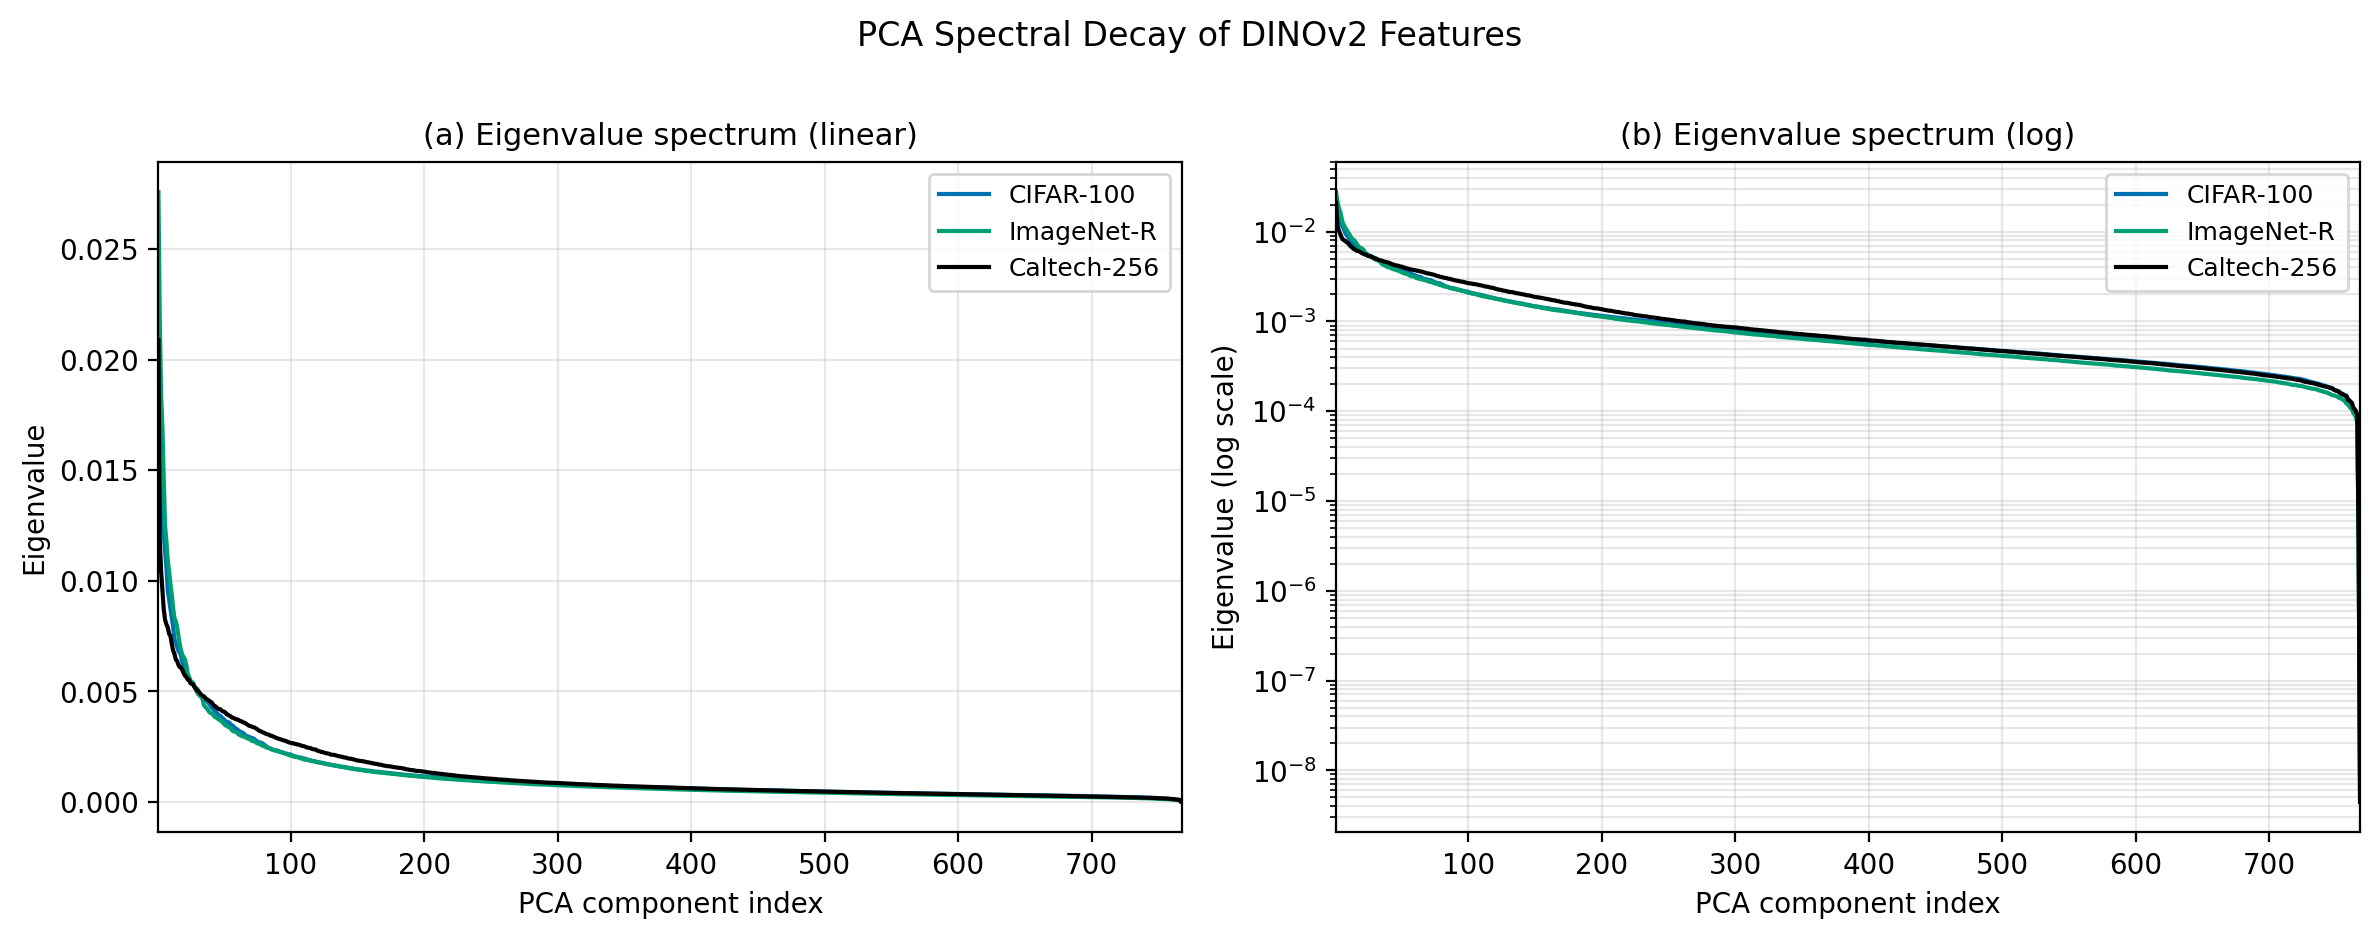
\includegraphics[width=0.97\linewidth]{imagenes/results/pca_eigenvalues.png}
	\caption{PCA spectral decay of the $\ell_2$-normalised DINOv2 features. \textbf{(a)} Individual \% variance explained per component: steep decay over the first $\sim\!50$ components, near-zero contribution thereafter. \textbf{(b)} Cumulative \% variance explained: dashed reference lines mark 50, 80, 90 and 95\,\%; annotated $n$ values show how many components suffice to reach 90\,\% on each dataset. Despite the $d=768$ embedding space, $90\,\%$ of the variance is captured by fewer than 130 components on every benchmark.}
	\label{fig:pca_eigenvalues}
\end{figure}

One notable feature of this spectrum is how similar it looks across very different image distributions. As shown in Figure~\ref{fig:pca_eigenvalues}, the decay curves for Split CIFAR-100, Split ImageNet-R, and Split Caltech-256 overlap almost exactly, so DINOv2 spreads variance across its coordinates in roughly the same way whether it is processing low-resolution natural images, artistic renditions, or high-resolution object photography. Because of this, there is no need to tune the dimensionality separately for each dataset, and the same probabilistic modelling layer can be used across all of them.

\subsection{Spectral Properties of the Foundation Embeddings}
\label{sec:an:spectrum}

The spectrum in Figure~\ref{fig:pca_eigenvalues} shows three consistent patterns across the DINOv2 feature space.

First, all three benchmarks allocate variance in a similar multi-stage way. The first principal component accounts for roughly 8\%--10\% of the total variance, followed by a sharp decay over the first $\sim\!50$ dimensions that together capture 36\%--40\% of the global variance. Beyond that point, the spectrum flattens into a long tail that decays slowly across the remaining 700+ coordinates.

Second, there is no abrupt cutoff in the spectrum. Most of the discriminative signal sits in a moderate-dimensional subspace, but it is not confined to it entirely: some real variability is spread across the whole ambient space. This is why we use a full, high-dimensional ($d=768$) generative model instead of a truncated, PCA-reduced one by default.

Third, and independently of this global spectrum, the effective rank of any per-class empirical covariance matrix is bounded above by $n_c - 1$, since at most $n_c - 1$ directions can be populated from $n_c$ centred observations. When $n_c < d$, this bound alone forces rank deficiency, and it is the root cause of the numerical instability we saw earlier in unconstrained full-covariance estimation. The next subsection tests directly whether the concentration of variance shown here can be used to work around it.

\subsection{Empirical Validation via Subspace Compression Tracking}
\label{sec:pca_cl_results}

If most of the variance really does sit in a moderate-dimensional subspace, compressing the features before classification should recover most of the rank deficiency problem discussed above, at the cost of throwing away only the low-variance tail. To test this, we project the DINOv2 embeddings down to $d=64$ and $d=256$ dimensions and re-run the class-incremental classifiers on the compressed features. Table~\ref{tab:pca_accuracy} reports the average accuracy once every class has been added, across three independent class-ordering runs. As with the uncompressed results, the class-conditional statistics come from a fixed training partition, so the standard deviation is zero across all cells: which order the classes arrive in does not change where the estimator converges.

\begin{table}[htbp]
	\centering
	\caption{Final average accuracy (\%) of the Gaussian continual-learning classifier after projecting DINOv2 embeddings to $d\!\in\!\{64,\,256\}$ dimensions via PCA. \emph{Diag}: diagonal covariance; \emph{Full}: full covariance with adaptive ridge regularisation. Higher is better.}
	\label{tab:pca_accuracy}
	\small
	\setlength{\tabcolsep}{5pt}
	\begin{tabular}{l|ccc|ccc}
		\toprule
		& \multicolumn{3}{c|}{\textbf{PCA $d=64$}} & \multicolumn{3}{c}{\textbf{PCA $d=256$}} \\
		\textbf{Benchmark} & Diag & Full & MOG4-Shared & Diag & Full & MOG4-Shared \\
		\midrule
		CIFAR-100      & 78.48 & \textbf{83.05} & 82.24 & 85.22 & 82.29 & \textbf{88.16} \\
		ImageNet-R     & 64.04 & 49.65 & \textbf{66.84} & 71.79 & 61.25 & \textbf{77.06} \\
		Caltech-256    & 87.20 & 43.40 & \textbf{90.58} & 90.01 & 91.09 & \textbf{94.42} \\
		\bottomrule
	\end{tabular}
\end{table}

The behavior across dimensionalities maps directly onto the shape of the spectrum described above. Scaling the PCA dimensionality from $d=64$ to $d=256$ lifts Diag-Cov's accuracy on every benchmark ($+6.7$\,pp on Split CIFAR-100, $+7.8$\,pp on Split ImageNet-R, $+2.8$\,pp on Split Caltech-256), confirming that although fewer than 130 components already capture 90\% of the variance, the remaining low-variance tail still holds fine-grained information that helps resolve close class boundaries.

MOG4-Shared benefits from this compression even more than Diag-Cov does. At $d=256$ it is the best of the three methods on every benchmark ($88.16\%$ on CIFAR-100, $77.06\%$ on ImageNet-R, $94.42\%$ on Caltech-256), and at $d=64$ it already leads on ImageNet-R and Caltech-256, trailing Full-Cov by less than a point on CIFAR-100 ($82.24\%$ vs. $83.05\%$). This follows from the same mechanism discussed in Section~\ref{sec:an:homoscedasticity}: MOG4-Shared estimates a single covariance from the pooled residuals of every active class, so compressing the features still leaves it with plenty of data to estimate that one covariance well. Full-Cov, by contrast, has to fit a separate covariance per class from a much smaller sample, which is exactly what causes it to struggle under compression, as the next subsection shows in more detail.

\subsection{Covariance Parameterisations and Subspace Interplay}
\label{sec:pca_covariance_interplay}

The gap between Diag-Cov and Full-Cov shows two sides of the same regularisation problem under data scarcity. On Split CIFAR-100 at $d=64$, compression actually helps Full-Cov: the sample budget ($n_c=400$) comfortably exceeds the projection dimension, so it can exploit stable off-diagonal correlations and beat Diag-Cov by $+4.6$\,pp. Expanding to $d=256$ reverses this into a $-2.9$\,pp deficit, since even within the leading part of the spectrum, the number of free parameters starts to outpace how much data is available.

This same effect causes a sharp drop for Full-Cov on the sample-starved streams of ImageNet-R ($n_c=40$) and Caltech-256 ($n_c=64$) under heavy compression. At $d=64$, Full-Cov's unconstrained covariance becomes rank-deficient, losing $14.4$\,pp on ImageNet-R and $43.8$\,pp on Caltech-256 relative to Diag-Cov. These gaps narrow as dimensionality expands to $d=256$, where Full-Cov eventually reaches the peak accuracy on Caltech-256 ($91.09\%$), but the pattern still shows that a linear dimensionality reduction can distort per-class correlations whenever the sample budget stays close to the projection size. MOG4-Shared avoids this failure mode altogether, for the reason given above: it never has to estimate an independent covariance from a small, per-class sample in the first place.

\section{Validating the DINOv2 Gaussianity Assumption}
\label{sec:gaussianity_results}

Chapter~\ref{ch:gaussian_space} checked Gaussianity at two levels: per-dimension, whether each coordinate on its own looks Gaussian, and per-class, whether the full, high-dimensional feature vector of each class does. Here we apply both checks to the actual DINOv2 embeddings used throughout this thesis, using the training split of each benchmark.

\subsection{Per-Dimension Gaussianity}
\label{sec:uv_gaussianity}

\textbf{Shape moments.}
We compute the sample skewness and excess kurtosis defined in Chapter~\ref{ch:gaussian_space} for every (class $c$, dimension $j$) pair.

\begin{table}[htb]
    \centering
    \caption{Per-dimension Gaussianity statistics over all $(C \times d)$ (class, dimension) pairs per dataset ($d=768$). $|\!\mathrm{Skew}|_\mu$ and $|\!\mathrm{Kurt}|_\mu$ are mean absolute values; $\mathbb{P}[\cdot]$ is the fraction of pairs satisfying each cut-off.}
    \label{tab:gaussianity_stats}
    \scriptsize
    \setlength{\tabcolsep}{4pt}
    \begin{tabular}{lcc cc cc}
        \toprule
        \textbf{Dataset} & \textbf{pairs} & $|\!\mathrm{Skew}|_\mu$ & $\mathrm{Skew}_\sigma$ & $\mathbb{P}[|\mathrm{Skew}|{<}0.5]$ & $|\!\mathrm{Kurt}|_\mu$ & $\mathbb{P}[|\mathrm{Kurt}|{<}1]$ \\
        \midrule
        CIFAR-100   & 76,800  & $0.181$ & $0.236$ & $0.961$ & $0.264$ & $0.982$ \\
        ImageNet-R  & 153,600 & $0.269$ & $0.348$ & $0.859$ & $0.432$ & $0.924$ \\
        Caltech-256 & 192,000 & $0.360$ & $0.472$ & $0.747$ & $0.659$ & $0.822$ \\
        \bottomrule
    \end{tabular}
\end{table}

Table~\ref{tab:gaussianity_stats} reports aggregate statistics. Mean skewness is essentially zero on all benchmarks ($|\overline{\mathrm{Skew}}| \le 0.002$). The fraction of pairs satisfying $|\mathrm{Skew}|<0.5$ drops from $96.1\%$ on CIFAR-100 to $74.7\%$ on Caltech-256, reflecting the smaller per-class sample count and greater visual diversity of the latter.

\textbf{D'Agostino--Pearson test.}
We apply the joint hypothesis test defined in Chapter~\ref{ch:gaussian_space}, rejecting $H_0$ at $\alpha=0.05$, and report the fraction of pairs passing in Table~\ref{tab:gaussianity_normaltest}. With $\bar{n}_c \approx 400$, $120$, and $90$ for CIFAR-100, ImageNet-R, and Caltech-256 respectively, the test gets stricter as the sample grows, so even small, harmless departures from normality get flagged on the larger datasets; even so, $70$--$81\%$ of all pairs pass it, and the relaxed criterion from Chapter~\ref{ch:gaussian_space} ($|\mathrm{Skew}|<1$ and $|\mathrm{Kurt}|<1$) is satisfied by $82$--$98\%$.

\begin{table}[htb]
    \centering
    \caption{Per-feature normality tests on the training split (fractions of $(C \times d)$ pairs). \emph{normaltest}: D'Agostino--Pearson $\chi^2_2$ at $\alpha{=}0.05$. \emph{relaxed}: $|\mathrm{Skew}|<1$ and $|\mathrm{Kurt}|<1$ simultaneously.}
    \label{tab:gaussianity_normaltest}
    \scriptsize
    \setlength{\tabcolsep}{6pt}
    \begin{tabular}{lccc}
        \toprule
        \textbf{Dataset} & \textbf{Normaltest (\%)} & \textbf{Relaxed (\%)} & \textbf{Both (\%)} \\
        \midrule
        CIFAR-100   & $70.0$ & $97.8$ & $70.0$ \\
        ImageNet-R  & $80.8$ & $91.6$ & $79.7$ \\
        Caltech-256 & $73.4$ & $82.3$ & $71.3$ \\
        \bottomrule
    \end{tabular}
\end{table}

\textbf{Henze--Zirkler test per dimension.}
\phantomsection\label{sec:uv_hz_gaussianity_results}
As a stricter check, we also apply the univariate Henze--Zirkler (HZ) test defined in Chapter~\ref{ch:gaussian_space} independently to every $(c,j)$ pair, using $d=1$ and the same finite-sample expectation and bandwidth given there.

\begin{table}[htb]
	\centering
	\caption{Summary results from computing the univariate Henze--Zirkler test statistic over all $(C \times d)$ class-dimension pairs on the training split. $\mathbb{E}_{H_0}[T_{\mathrm{HZ}}]$ is the theoretical expectation under perfect normality, as defined in Chapter~\ref{ch:gaussian_space}, evaluated at the per-class sample size $n_c$.}
	\label{tab:gaussianity_hz_univariate}
	\scriptsize
	\setlength{\tabcolsep}{4pt}
	\begin{tabular}{lcc c}
		\toprule
		\textbf{Dataset} & $\tilde{n}_c$ & $\mathbb{E}_{H_0}[T_{\mathrm{HZ}}]$ & $T_{\mathrm{HZ}}$ mean\,$\pm$\,std \\
		\midrule
		CIFAR-100  & 500 & $\approx 0.04$ & $0.00052 \pm 0.00095$ \\
		ImageNet-R  & 137 & $\approx 0.06$ & $0.00134 \pm 0.00210$  \\
		Caltech-256 & 100 & $\approx 0.07$ & $0.00234 \pm 0.00379$  \\
		\bottomrule
	\end{tabular}
\end{table}

Taken together, these three diagnostics agree: the individual coordinates of the foundation feature vectors have symmetric shapes, near-zero skewness, and little excess kurtosis, and the observed HZ scores sit orders of magnitude below their theoretical $H_0$ expectation. Every marginal, taken on its own, looks close to Gaussian.

\subsection{Per-Class Gaussianity}
\label{sec:mv_gaussianity_results}

Per-dimension normality is necessary but not sufficient: a set of coordinates can each look Gaussian on their own while still not being jointly Gaussian, so we now test each class's full $d=768$-dimensional feature vector at once, using the same HZ statistic as before but with $d$ set to the full embedding dimension. As explained in Chapter~\ref{ch:gaussian_space}, this runs into the same problem as everywhere else in this thesis: since $n_c < d$ for every benchmark, the full covariance matrix needed for the standard version of the test cannot be inverted.

We work around this the same way: by using a diagonal version of the covariance, so only the $d$ per-coordinate variances need to be inverted instead of the full matrix. This changes what to expect under $H_0$ as well. In the univariate case above, a Gaussian coordinate gives $T_{\mathrm{HZ}}$ close to $0$; here, because $d$ is large, the same expectation formula pushes the reference value close to $1$ instead. Table~\ref{tab:gaussianity_hz} shows that all three benchmarks concentrate tightly around $T_{\mathrm{HZ}} = 1$, right where a Gaussian class should land under this diagonal test.

\begin{table}[htb]
    \centering
    \caption{Summary results from computing the diagonal HZ test statistic over all classes in the ambient foundation feature space ($d=768$), using all available training samples. Values concentrated near $T_{\mathrm{HZ}} \approx 1.00$ indicate convergence toward empirical multivariate Gaussianity under the feature-independence assumption.}
    \label{tab:gaussianity_hz}
    \scriptsize
    \setlength{\tabcolsep}{4pt}
    \begin{tabular}{lcc c}
        \toprule
        \textbf{Dataset} & $C$ & $T_{\mathrm{HZ}}$ mean\,$\pm$\,std \\
        \midrule
        CIFAR-100   & 100 & $1.0002 \pm 0.0020$  \\
        ImageNet-R  & 200 & $1.0033 \pm 0.0073$ \\
        Caltech-256 & 250 & $1.0016 \pm 0.0089$ \\
        \bottomrule
    \end{tabular}
\end{table}

As already noted in Chapter~\ref{ch:gaussian_space}, restricting this test to a diagonal covariance means it cannot guarantee full, unconstrained multivariate Gaussianity, where every pair of dimensions is allowed to correlate freely. But given how little data is available per class relative to the embedding dimension, this diagonal version is the only one we can actually compute, and it works as a reasonable stand-in for the stronger, unconstrained test. The consistent convergence to $T_{\mathrm{HZ}} \approx 1.00$ across all three benchmarks is what supports using independent-feature probabilistic classifiers on this embedding space.

\subsection{Empirical Validation of the Gaussian Assumption}
\label{sec:an:gauss}

The Gaussianity tests above confirm that the per-coordinate normality assumption is well supported across all three benchmarks: 96.1\,\% of CIFAR-100 coordinates, 85.9\,\% of ImageNet-R, and 74.7\,\% of Caltech-256 satisfy the informal symmetry cut-off $|\text{Skew}|<0.5$. The key distinction between the two covariance estimators follows directly from the $n_c < d$ regime. The \textbf{Diag-Cov} model estimates only $d$ parameters per class and is therefore always well-conditioned; its squared Mahalanobis distances are broadly distributed near the theoretical $\chi^2_{d=768}$ mode, with dispersion growing from CIFAR-100 to Caltech-256 in line with the heavy-tail ordering of Table~\ref{tab:gaussianity_stats}. The \textbf{Full-Cov} model, by contrast, requires estimating a $d\times d$ matrix from $n_c < d$ samples: the resulting covariance is rank-deficient, the eigenvalues outside the spanned subspace collapse to the regularisation floor, and the quadratic form becomes degenerate, producing a sharp spike at $\overline{n_c}-1$ (approximately 498, 168, and 103 on CIFAR-100, ImageNet-R, and Caltech-256 respectively) rather than spreading across the $\chi^2_{768}$ support. This problem comes from the \emph{estimator}, not from the data: the per-coordinate distributions are near-Gaussian, as shown above. Keeping inter-feature correlations while avoiding rank deficiency is still an open challenge; the hybrid variant is one practical way to balance the two.

For \textbf{MOG4-Shared}, the same $n_c < d$ regime explains why it avoids this trade-off in the first place. Because MOG4-Shared estimates a single covariance from the pooled residuals of every active class rather than one covariance per class, it is never forced to invert a $d\times d$ matrix built from a single class's small sample, so it does not run into the rank-deficiency spike that hurts Full-Cov. On top of that, letting each class use up to four centroids means a class does not need its own feature distribution to be a single, unimodal Gaussian to be modelled well: a mixture of a few Gaussians can still fit a class whose marginals depart from normality more than the ones tested here. This is consistent with MOG4-Shared's results throughout this chapter, and it is one more reason it holds up better than either single-covariance model on its own.

\section{Computational Cost and Practical Considerations}
\label{sec:computational_requirements}
\phantomsection\label{sec:an:other}

Weighing accuracy against computational overhead matters for judging whether a lifelong learning framework is actually practical to run. Table~\ref{tab:computational_requirements} reports the inference cost of the Gaussian classification layer, in floating-point operations (FLOPs), needed to score a single pre-embedded test query against every active category once all tasks have been added.

Each covariance parameterisation has a different, predictable cost:
\begin{itemize}
	\item \textbf{Diag-Cov} scores each class with an element-wise weighted squared Euclidean distance, so the cost grows linearly, $\mathcal{O}(C \cdot d)$, where $C$ is the number of active classes and $d=768$ is the feature dimension.
	\item \textbf{Full-Cov} (and, by extension, Hybrid-Cov, whose Mahalanobis term uses the same Cholesky-based whitening) needs a full matrix--vector multiplication per class to account for the off-diagonal correlations, so its cost grows quadratically, $\mathcal{O}(C \cdot d^2)$.
	\item \textbf{MOG4-Shared} scores each class's up-to-four centroids against the one shared covariance, so its cost is $\mathcal{O}(C \cdot \bar{K} \cdot d^2)$, where $\bar{K}$ is the average number of centroids per class. This puts it between Diag-Cov and a hypothetical unshared, full-mixture model in cost, closer to Full-Cov in practice since both are dominated by the same $d^2$ term.
\end{itemize}

\begin{table}[htbp]
	\centering
	\caption{Inference cost of the Gaussian classification stage once every class has been added, in floating-point operations (FLOPs) per query, for the two dominant covariance parameterisations and for MOG4-Shared. For reference, a single forward pass of the DINOv2 ViT-B/14 feature extractor requires approximately $17.56$ GFLOPs.}
	\label{tab:computational_requirements}
	\small
	\setlength{\tabcolsep}{8pt}
	\begin{tabular}{lccc}
		\toprule
		\textbf{Benchmark} & \textbf{Diag-Cov} & \textbf{Full-Cov} & \textbf{MOG4-Shared} \\
		\midrule
		Split CIFAR-100   & $0.46$ MFLOPs & $0.12$ GFLOPs & $0.42$ GFLOPs \\
		Split ImageNet-R  & $0.92$ MFLOPs & $0.24$ GFLOPs & $0.31$ GFLOPs \\
		Split Caltech-256 & $1.15$ MFLOPs & $0.29$ GFLOPs & $0.58$ GFLOPs \\
		\bottomrule
	\end{tabular}
\end{table}

Even the most demanding case in the table, MOG4-Shared on the 250 classes of Split Caltech-256, needs only $0.58$ GFLOPs. That is still under $4\%$ of the cost of a single forward pass through the DINOv2 ViT-B/14 feature extractor itself ($\approx 17.56$ GFLOPs). So while MOG4-Shared is consistently more expensive than Diag-Cov and, on two of the three benchmarks, than Full-Cov too, the frozen backbone is still what dominates the total cost by a wide margin: whichever covariance estimator is used, it adds essentially no overhead at inference time.

\subsection{Computational Footprint and Practical Scalability}
\label{sec:an:compute}

These FLOPs numbers also show up as a real advantage in wall-clock time. On Split CIFAR-100, adding a newly encountered task to our framework takes about two minutes on a standard consumer-grade GPU, and that time is spent entirely on a single, deterministic pass of feature extraction over the raw images, needed to compute the class statistics.

Prompt-tuning methods reported in the literature typically need 10--30 minutes of training per task on similar hardware, since they backpropagate through a pool of learned prompts over several epochs. Because our framework never backpropagates and never needs a rehearsal buffer, it trains 5--15$\times$ faster, which makes it a reasonable option for low-resource or decentralized edge deployment.

\subsection{Limitations and Architectural Open Questions}
\label{sec:an:limits}

The empirical results support the efficiency and calibration of this frozen generative approach, but three limitations are worth being explicit about.

First, the current evaluation pipeline assumes that exact task boundaries are given during training to partition incoming batches. Relaxing this constraint to support task-free continual learning is an important next step, to test whether the decoupled Gaussian updates stay robust when categorical boundaries are blurred or interleaved.

Second, our experimental validation has focused only on visual classification streams. Although the underlying generative mechanics are in principle agnostic to the input modality, running a parallel validation on transformer-encoded text or speech embeddings is needed to check whether the clean Gaussian behavior observed here generalizes to other representation spaces.

Third, an interesting extension is using the well-behaved calibration profiles of our independent configurations for open-world discovery. The strong overconfidence of the Full covariance model makes its predictive metrics unreliable outside its closed label space. However, the well-calibrated Predictive Entropy and Probability Margin of the Diagonal model could be used directly as natural out-of-distribution scores. Investigating this could show whether the framework can flag novel, unlearned semantic categories while keeping its existing performance.

\section{Summary of Findings and Practical Recommendations}
\label{sec:an:summary}

The results in this chapter give an overall picture of the behavior, computational cost, and limitations of closed-form generative classifiers built on frozen foundation embeddings. Taken together, they show that class-incremental learning, in this setting, can be treated as a density-estimation problem in a stationary representation space rather than as a fight against forgetting. The DINOv2 feature manifold agrees well with the marginal normality assumption, passing coordinate-level Gaussianity thresholds for $96\,\%$ of dimensions in Split CIFAR-100, $86\,\%$ in Split ImageNet-R, and $75\,\%$ in Split Caltech-256, and because the representation stays stable as tasks accumulate, the resulting decision boundaries compete with optimization-heavy, prompt-based architectures while staying deterministic, closed-form, and gradient-free.

The classification ceiling of this framework is set mainly by the upstream feature extractor, not by the downstream classifier, as shown by the large performance gaps across different visual backbones in Section~\ref{sec:backbone_results}. Separately from the choice of backbone, classification error is not spread evenly across classes: it concentrates in a small, heavy-tailed set of pairs, under $0.2\,\%$ of all class combinations, where the pairwise Bhattacharyya distance drops below a critical threshold ($D_B < 20$). These are cases of near-synonymous or visually continuous categories, such as \textit{boy}/\textit{girl} at low resolution, or \textit{top-hat}/\textit{cowboy-hat} and \textit{bow\_tie}/\textit{scarf} under domain shift, where second-order statistics alone cannot pull the classes apart. What looks like forgetting in a frozen stream is really just newly introduced categories landing close to ones already learned.

Which covariance estimator to use depends on the sample budget and how homogeneous the incoming stream is. MOG4-Shared is the strongest general-purpose default: pooling one covariance across every active class keeps it numerically stable even when classes come from very different, unevenly sampled sources, and letting each class use up to four centroids still captures visual variety that a single Gaussian would miss, which is why it comes out ahead across every benchmark in Table~\ref{tab:combined_benchmarks}. When the per-class sample size comfortably exceeds the feature dimensionality and the stream is homogeneous, Full-Cov (or Hybrid-Cov under tighter sample budgets) can match or edge it out at a lower computational cost, since it captures off-diagonal correlations directly without needing the shared-covariance machinery. But once the stream mixes sources with very different sample sizes, as in the Joint benchmark, unconstrained per-class covariances break down, and a shared covariance, ideally paired with MOG4-Shared's extra centroids, is the only reliable choice.

These results support the central idea of this thesis: that lifelong learning, in this setting, can be handled as static statistical modelling instead of ongoing parameter optimization. Because the framework only ever computes frozen sufficient statistics, representation drift is not possible by construction, and the practical decision comes down to picking the covariance parameterisation, MOG4-Shared by default, one of the others when its sample budget and computational cost make more sense, that fits the sample density and semantic granularity of the deployment scenario. Chapter~\ref{ch:conclusion} builds on this to discuss the system-level conclusions and the open questions around representation alignment raised here.
\chapter{Conclusion}
\label{ch:conclusion}

This thesis revisited class-incremental learning (CIL) in the context of modern visual foundation models, arguing that once representations are frozen and sufficiently discriminative, the central challenge of CIL shifts from protecting network parameters against interference to properly modelling the statistical structure of a stationary embedding space. We formalised this shift by formulating incremental learning as the recursive, gradient-free estimation of class-conditional Gaussian densities in the embedding space of a frozen DINOv2 backbone. Each class is represented entirely by its sufficient statistics---a mean vector and a covariance matrix---which are updated in closed form as new samples arrive, without backpropagation, replay buffers, exemplar storage, or prompt parameters, and without ever modifying the statistics of a previously learned class. This design eliminates catastrophic forgetting by construction rather than by mitigation, and it is the structural reason why the forgetting scores reported throughout Chapter~\ref{ch:results} reflect increasing classification difficulty as the class set grows rather than any degradation of previously acquired knowledge.

Empirically, this conceptually simple formulation is competitive with the strongest prompt-based state of the art. Our full-covariance and mixture-of-Gaussian configurations match ConvPrompt on Split CIFAR-100 ($88.87\,\%$) without any trainable parameters or optimisation during incremental learning, and the Full-Cov and Hybrid-Cov estimators outperform every prompt-based baseline reported on Split Caltech-256 ($94.93\,\%$ versus the best prompt-based result of $92.50\,\%$). This level of accuracy is achieved at a computational cost for the classification stage below $0.3$ GFLOPs in the worst case---more than fifty times smaller than the $\approx 17.56$ GFLOPs required for a single forward pass of the DINOv2 backbone---so that the probabilistic classification layer introduces only marginal overhead relative to feature extraction, and requires none of the gradient updates that prompt-based competitors perform at every incremental task.

Beyond the accuracy figures, this thesis provided a rigorous statistical validation of the assumption that underlies the entire framework. Combining moment-based diagnostics with formal hypothesis tests---the D'Agostino--Pearson omnibus test for univariate normality and a diagonal adaptation of the Henze--Zirkler test for multivariate normality under severe rank deficiency---confirmed that the marginal feature distributions of a self-supervised foundation encoder are consistently, if not perfectly, Gaussian across three visually heterogeneous benchmarks: $70$--$81\,\%$ of all (class, dimension) pairs pass the strict D'Agostino--Pearson test, and the diagonal multivariate Henze--Zirkler statistic converges tightly to its Gaussian reference value of $1$ on every dataset. The complementary Bhattacharyya-distance analysis established a direct, quantitative link between inter-class separability and the achievable classification accuracy: over $99.8\,\%$ of all class pairs on every benchmark exceed a separability threshold of $D_B=50$, while the small minority of pairs that fall below $D_B=20$---semantic or visual near-synonyms such as \textit{boy}/\textit{girl}, \textit{bow\_tie}/\textit{scarf}, and \textit{top-hat}/\textit{cowboy-hat}---account for essentially the entirety of the residual classification error identified in the confusion-pattern analysis of Chapter~\ref{ch:analysis}. This is, to our knowledge, one of the first attempts in the class-incremental learning literature to connect a formal probabilistic error bound directly to the specific, named class pairs that a deployed classifier will actually confuse.

This thesis further showed that the reliability of full-rank covariance modelling is itself a matter of numerical care, not only of statistical assumption. Computing the precision matrix and log-determinant of the Full-Cov and Hybrid-Cov estimators via a Cholesky-based decomposition, rather than via an eigendecomposition with a hard eigenvalue floor, avoids a substantial artefact that would otherwise depress the Full-Cov accuracy on Split Caltech-256 by nearly five accuracy points and produce misleadingly optimistic results on the 30-task Joint benchmark. The results present a clear and interpretable picture: full-rank covariance estimation is highly beneficial whenever the per-class sample budget is adequate and homogeneous across classes, but the Joint benchmark's collapse of Full-Cov and Hybrid-Cov to $59.35\,\%$ is not a weakness of the estimator---it is a confirmation that covariance parameterisation must be matched to the sample-size regime of the deployment scenario, precisely as the Shared-covariance variants, which pool statistics across classes of heterogeneous rank, demonstrate by becoming the strongest estimators in that same setting ($81.49\,\%$).

These results, taken together, support the view that in the visual foundation-model era, the central challenge of class-incremental learning is no longer protecting network parameters from catastrophic interference but correctly modelling and exploiting the statistical geometry of a stable representation space. The success of a classical, decades-old statistical tool---the multivariate Gaussian classifier---in this modern setting is not a coincidence: it is made possible by the qualitative change that large-scale self-supervised pretraining has produced in the topology of visual embedding spaces. By decoupling representational plasticity from semantic categorisation, stable and well-behaved foundation features eliminate representation drift by construction, allowing lifelong visual recognition to be reframed as an ongoing, closed-form problem of probability density estimation rather than an ongoing problem of parameter optimisation.

\paragraph{Limitations.} A key limitation of the present work follows directly from the discussion of Chapter~\ref{ch:analysis} and deserves explicit restatement here: the framework's residual error is structurally bounded by the semantic resolution of the upstream encoder. No choice of covariance estimator or mixture model evaluated in this thesis can fully resolve a class pair whose Bhattacharyya distance and Euclidean mean separation are both near zero, since such a pair reflects a genuine ambiguity in the frozen feature space rather than a deficiency of the downstream classifier.

\section{Future Work}

Several natural extensions of the framework deserve further investigation, building on the longer-term research directions identified in this thesis.

\textbf{Targeted Representation Alignment for Lingering Confusion Sinks.} 
Our failure diagnostics isolated a minute, semantically coherent subset of class pairs (e.g., \textit{boy}/\textit{girl} or \textit{top-hat}/\textit{cowboy-hat}) that account for almost the entire residual error of the system due to their near-zero mean separation ($d_E \to 0$). Because this crowding is an inherent property of the upstream embedding space, it cannot be resolved by downstream parametric tuning. Future research should investigate lightweight, targeted representation alignment. Instead of re-training the entire deep backbone, a contrastive or metric-learning objective can be applied exclusively to the low-$D_B$ class pairs flagged by our statistical diagnostics. This targeted adjustment can local-stretch the decision surface for highly ambiguous categories, maximizing class separability without disrupting the global stationarity of the remaining representation space.

\textbf{Structured Covariance Parameterisation Under Highly Heterogeneous Sample Budgets.} 
The Hybrid-Cov estimator successfully decouples the Mahalanobis shape component from the log-normalisation volume term, providing a stable baseline on homogeneous streams. However, as demonstrated by the Joint benchmark collapse, unconstrained second-order parameters break down when forced to compare data-rich classes directly against sample-starved categories. To alleviate this sensitivity, future work should develop structured precision matrices that dynamically adapt their complexity to individual sample counts.

\textbf{Probabilistic Uncertainty Calibration.} 
Our calibration metrics reveal that full-covariance parameterisations suffer from structural over-confidence, as the estimated distribution volumes tend to collapse around scarce sample clusters. This miscalibration reduces the trustworthiness of downstream probability scores in safety-critical deployment environments. Future iterations should implement post-hoc calibration layers designed for closed-form streams, such as multi-class temperature scaling or conformal prediction frameworks. By computing distribution-free prediction intervals based on historical validation residuals, the system can provide mathematically guaranteed error bounds alongside its standard maximum-a-posteriori assignments.


\textbf{Gradient-Free Spatial Object Detection.} 
A natural functional scaling for this architecture is extending its reach from global scene classification to localized object detection. Traditional multi-stage object detectors rely on intensive backpropagation to optimize region proposal networks (RPNs) and bounding-box regressors, creating severe computational bottlenecks. Future work should bypass these requirements by exploiting the localized patch tokens natively generated during a single forward pass of the DINOv2 backbone. By applying simple mathematical decompositions—such as localized principal component analysis or spatial attention routing—directly onto these frozen spatial features, areas of interest can be isolated and classified in a single, gradient-free pass, preserving the lightweight, deterministic philosophy of this thesis.

\textbf{Autonomous Open-World Discovery.} 
Because this framework computes closed-form sufficient statistics natively, it provides a well-behaved predictive entropy and Log-Gap score for every incoming sample. This capability can be leveraged to shift the system from a closed-set classifier toward an open-world discovery framework. Since the uncertainty boundaries of the Diag-Cov branch remain structurally stable when new categories are introduced, establishing an adaptive out-of-distribution (OOD) threshold would allow the model to autonomously isolate unknown entities. Once flagged, these unfamiliar clusters can be accumulated and parameterized as new Gaussian classes in closed form, expanding the label space without requiring external supervision or manual task boundaries.



\nocite{*}
\bibliographystyle{ieeetr}
\bibliography{bibliografia}

% opcional ...
%\begin{appendices}
%\input{Capitulos/AnexoA} % opcional
%\input{Capitulos/AnexoB} % opcional
%\end{appendices}
\end{document}
